% Options for packages loaded elsewhere
\PassOptionsToPackage{unicode}{hyperref}
\PassOptionsToPackage{hyphens}{url}
\PassOptionsToPackage{dvipsnames,svgnames,x11names}{xcolor}
%
\documentclass[
]{book}
\usepackage{amsmath,amssymb}
\usepackage{iftex}
\ifPDFTeX
  \usepackage[T1]{fontenc}
  \usepackage[utf8]{inputenc}
  \usepackage{textcomp} % provide euro and other symbols
\else % if luatex or xetex
  \usepackage{unicode-math} % this also loads fontspec
  \defaultfontfeatures{Scale=MatchLowercase}
  \defaultfontfeatures[\rmfamily]{Ligatures=TeX,Scale=1}
\fi
\usepackage{lmodern}
\ifPDFTeX\else
  % xetex/luatex font selection
\fi
% Use upquote if available, for straight quotes in verbatim environments
\IfFileExists{upquote.sty}{\usepackage{upquote}}{}
\IfFileExists{microtype.sty}{% use microtype if available
  \usepackage[]{microtype}
  \UseMicrotypeSet[protrusion]{basicmath} % disable protrusion for tt fonts
}{}
\makeatletter
\@ifundefined{KOMAClassName}{% if non-KOMA class
  \IfFileExists{parskip.sty}{%
    \usepackage{parskip}
  }{% else
    \setlength{\parindent}{0pt}
    \setlength{\parskip}{6pt plus 2pt minus 1pt}}
}{% if KOMA class
  \KOMAoptions{parskip=half}}
\makeatother
\usepackage{xcolor}
\usepackage{color}
\usepackage{fancyvrb}
\newcommand{\VerbBar}{|}
\newcommand{\VERB}{\Verb[commandchars=\\\{\}]}
\DefineVerbatimEnvironment{Highlighting}{Verbatim}{commandchars=\\\{\}}
% Add ',fontsize=\small' for more characters per line
\usepackage{framed}
\definecolor{shadecolor}{RGB}{248,248,248}
\newenvironment{Shaded}{\begin{snugshade}}{\end{snugshade}}
\newcommand{\AlertTok}[1]{\textcolor[rgb]{0.94,0.16,0.16}{#1}}
\newcommand{\AnnotationTok}[1]{\textcolor[rgb]{0.56,0.35,0.01}{\textbf{\textit{#1}}}}
\newcommand{\AttributeTok}[1]{\textcolor[rgb]{0.13,0.29,0.53}{#1}}
\newcommand{\BaseNTok}[1]{\textcolor[rgb]{0.00,0.00,0.81}{#1}}
\newcommand{\BuiltInTok}[1]{#1}
\newcommand{\CharTok}[1]{\textcolor[rgb]{0.31,0.60,0.02}{#1}}
\newcommand{\CommentTok}[1]{\textcolor[rgb]{0.56,0.35,0.01}{\textit{#1}}}
\newcommand{\CommentVarTok}[1]{\textcolor[rgb]{0.56,0.35,0.01}{\textbf{\textit{#1}}}}
\newcommand{\ConstantTok}[1]{\textcolor[rgb]{0.56,0.35,0.01}{#1}}
\newcommand{\ControlFlowTok}[1]{\textcolor[rgb]{0.13,0.29,0.53}{\textbf{#1}}}
\newcommand{\DataTypeTok}[1]{\textcolor[rgb]{0.13,0.29,0.53}{#1}}
\newcommand{\DecValTok}[1]{\textcolor[rgb]{0.00,0.00,0.81}{#1}}
\newcommand{\DocumentationTok}[1]{\textcolor[rgb]{0.56,0.35,0.01}{\textbf{\textit{#1}}}}
\newcommand{\ErrorTok}[1]{\textcolor[rgb]{0.64,0.00,0.00}{\textbf{#1}}}
\newcommand{\ExtensionTok}[1]{#1}
\newcommand{\FloatTok}[1]{\textcolor[rgb]{0.00,0.00,0.81}{#1}}
\newcommand{\FunctionTok}[1]{\textcolor[rgb]{0.13,0.29,0.53}{\textbf{#1}}}
\newcommand{\ImportTok}[1]{#1}
\newcommand{\InformationTok}[1]{\textcolor[rgb]{0.56,0.35,0.01}{\textbf{\textit{#1}}}}
\newcommand{\KeywordTok}[1]{\textcolor[rgb]{0.13,0.29,0.53}{\textbf{#1}}}
\newcommand{\NormalTok}[1]{#1}
\newcommand{\OperatorTok}[1]{\textcolor[rgb]{0.81,0.36,0.00}{\textbf{#1}}}
\newcommand{\OtherTok}[1]{\textcolor[rgb]{0.56,0.35,0.01}{#1}}
\newcommand{\PreprocessorTok}[1]{\textcolor[rgb]{0.56,0.35,0.01}{\textit{#1}}}
\newcommand{\RegionMarkerTok}[1]{#1}
\newcommand{\SpecialCharTok}[1]{\textcolor[rgb]{0.81,0.36,0.00}{\textbf{#1}}}
\newcommand{\SpecialStringTok}[1]{\textcolor[rgb]{0.31,0.60,0.02}{#1}}
\newcommand{\StringTok}[1]{\textcolor[rgb]{0.31,0.60,0.02}{#1}}
\newcommand{\VariableTok}[1]{\textcolor[rgb]{0.00,0.00,0.00}{#1}}
\newcommand{\VerbatimStringTok}[1]{\textcolor[rgb]{0.31,0.60,0.02}{#1}}
\newcommand{\WarningTok}[1]{\textcolor[rgb]{0.56,0.35,0.01}{\textbf{\textit{#1}}}}
\usepackage{longtable,booktabs,array}
\usepackage{calc} % for calculating minipage widths
% Correct order of tables after \paragraph or \subparagraph
\usepackage{etoolbox}
\makeatletter
\patchcmd\longtable{\par}{\if@noskipsec\mbox{}\fi\par}{}{}
\makeatother
% Allow footnotes in longtable head/foot
\IfFileExists{footnotehyper.sty}{\usepackage{footnotehyper}}{\usepackage{footnote}}
\makesavenoteenv{longtable}
\usepackage{graphicx}
\makeatletter
\def\maxwidth{\ifdim\Gin@nat@width>\linewidth\linewidth\else\Gin@nat@width\fi}
\def\maxheight{\ifdim\Gin@nat@height>\textheight\textheight\else\Gin@nat@height\fi}
\makeatother
% Scale images if necessary, so that they will not overflow the page
% margins by default, and it is still possible to overwrite the defaults
% using explicit options in \includegraphics[width, height, ...]{}
\setkeys{Gin}{width=\maxwidth,height=\maxheight,keepaspectratio}
% Set default figure placement to htbp
\makeatletter
\def\fps@figure{htbp}
\makeatother
\setlength{\emergencystretch}{3em} % prevent overfull lines
\providecommand{\tightlist}{%
  \setlength{\itemsep}{0pt}\setlength{\parskip}{0pt}}
\setcounter{secnumdepth}{5}
% definitions for citeproc citations
\NewDocumentCommand\citeproctext{}{}
\NewDocumentCommand\citeproc{mm}{%
  \begingroup\def\citeproctext{#2}\cite{#1}\endgroup}
\makeatletter
 % allow citations to break across lines
 \let\@cite@ofmt\@firstofone
 % avoid brackets around text for \cite:
 \def\@biblabel#1{}
 \def\@cite#1#2{{#1\if@tempswa , #2\fi}}
\makeatother
\newlength{\cslhangindent}
\setlength{\cslhangindent}{1.5em}
\newlength{\csllabelwidth}
\setlength{\csllabelwidth}{3em}
\newenvironment{CSLReferences}[2] % #1 hanging-indent, #2 entry-spacing
 {\begin{list}{}{%
  \setlength{\itemindent}{0pt}
  \setlength{\leftmargin}{0pt}
  \setlength{\parsep}{0pt}
  % turn on hanging indent if param 1 is 1
  \ifodd #1
   \setlength{\leftmargin}{\cslhangindent}
   \setlength{\itemindent}{-1\cslhangindent}
  \fi
  % set entry spacing
  \setlength{\itemsep}{#2\baselineskip}}}
 {\end{list}}
\usepackage{calc}
\newcommand{\CSLBlock}[1]{\hfill\break\parbox[t]{\linewidth}{\strut\ignorespaces#1\strut}}
\newcommand{\CSLLeftMargin}[1]{\parbox[t]{\csllabelwidth}{\strut#1\strut}}
\newcommand{\CSLRightInline}[1]{\parbox[t]{\linewidth - \csllabelwidth}{\strut#1\strut}}
\newcommand{\CSLIndent}[1]{\hspace{\cslhangindent}#1}
\ifLuaTeX
  \usepackage{selnolig}  % disable illegal ligatures
\fi
\usepackage{bookmark}
\IfFileExists{xurl.sty}{\usepackage{xurl}}{} % add URL line breaks if available
\urlstyle{same}
\hypersetup{
  pdftitle={Statistical Modelling},
  colorlinks=true,
  linkcolor={Maroon},
  filecolor={Maroon},
  citecolor={Blue},
  urlcolor={blue},
  pdfcreator={LaTeX via pandoc}}

\title{Statistical Modelling}
\usepackage{etoolbox}
\makeatletter
\providecommand{\subtitle}[1]{% add subtitle to \maketitle
  \apptocmd{\@title}{\par {\large #1 \par}}{}{}
}
\makeatother
\subtitle{A conceptual, visual and practical introduction}
\author{true}
\date{23 April, 2025}

\begin{document}
\maketitle

{
\hypersetup{linkcolor=}
\setcounter{tocdepth}{1}
\tableofcontents
}
\chapter*{Preface: what's the problem?}\label{preface-whats-the-problem}
\addcontentsline{toc}{chapter}{Preface: what's the problem?}

The world abounds with data - but scientific and investigative work does not \emph{begin} with data. It is true that data which is already available may give ideas and suggest hypotheses, but a serious project will start by thinking carefully about well defined objectives. In other words, scientific work begins with a clearly stated \emph{problem}.

Statistical modelling refers to the process by which we collect and use data to gain insight into the problem we have defined and to lead us towards a conclusion. In an interesting paper on scientific and statistical methods, MacKay and Oldford (\citeproc{ref-mackay_2000_statsci}{2000}) structured the process in the following broad steps, referred to by the acronym PPDAC. Some of the key questions which are likely to arise in each step have been highlighted.

\begin{itemize}
\tightlist
\item
  Problem

  \begin{itemize}
  \tightlist
  \item
    What are the key questions we would like to address?
  \item
    What is the context in which these questions are framed?
  \end{itemize}
\item
  Plan

  \begin{itemize}
  \tightlist
  \item
    How should our experiment be designed?
  \item
    What data should be collected and how much?
  \end{itemize}
\item
  Data

  \begin{itemize}
  \tightlist
  \item
    How should the data be checked for validity and consistency?
  \item
    What methods of visual exploration should we use?
  \end{itemize}
\item
  Analysis

  \begin{itemize}
  \tightlist
  \item
    How should an appropriate model be constructed?
  \item
    What does analysis of our model tell us about our problem?
  \end{itemize}
\item
  Conclusion

  \begin{itemize}
  \tightlist
  \item
    How should we report to others on our conclusions?
  \item
    What limitations and caveats should we highlight?
  \end{itemize}
\end{itemize}

This broad view of statistical modelling sets the agenda for the book.

There are many textbooks and resources available which discuss statistical modelling - why another one? This book aims takes a particular approach.

\begin{itemize}
\tightlist
\item
  The focus is on \textbf{conceptual} understanding of the main ideas behind statistical thinking and modelling. Some technical details are provided for those who are interested but engagement with this material is optional.
\item
  There is a strong theme of \textbf{visual} communication of both data and the concepts behind statistical models.
\item
  The approach is also \textbf{practical} with extensive reference to the widely used statistical computing environment R as a means of engaging with the concepts and implementing the methods discussed. In particular, there is extensive use of real datasets. The aim is to discuss interesting and scientifically important questions, where possible with the data used in published papers. As data become increasingly `open', datsets are read from publicly available sources wherever possible.
\end{itemize}

The target audience is those who need statistical methods to understand data. A good example is PhD students who are well motivated to analyse their experimental data. The scientific contexts of the examples come from a wide range of application areas, including the life sciences, the social sciences and topics of general interest. The aim is to provide examples which are both interesting and accessible, without the need for detailed technical knowledge of a particular area.

Throughout the book there are frequent references to the widely used statistical computing system R. It is possible to read this book without using R but it is primarily intended that the reader will use this powerful system to engage with the examples and exercises and with the whole process of statistical modelling. A description of how to install R, and the popular system RStudio which helpfully manages some aspects of the environment, is available immediately after this preface. A gentle introduction to R is provided in Chapter \ref{R-introduction}.

\textbf{Acknowledgements}

\textbf{Please note that this is a work in progress. Please forgive some rough edges in the presentation here and there.}

\chapter{Where do data come from?}\label{where-data}

Data can take many forms. Sometimes we are dealing with simple numbers, such as blood pressure measurements or age. Some data may consist of categories, such as country of origin or presence/absence of a characteristic of interest. Modern data can be much more sophisticated, arising in the form of images, temperature curves, three-dimensional surfaces or networks. This chapter focuses on relatively simple data forms but uses these to discuss some important principles of how data are collected and what they are able to tell us.

\section{Some examples of data}\label{examples-data}

\subsection{CO2 and global warming}\label{co2-and-global-warming}

One of the world's most pressing issue is climate change as a result of global warming. The levels of CO2 in the atmosphere are clearly implicated in this as a result of the `greenhouse' effect. Accurate monitoring of CO2 began in the late 1950's through the pioneering work of Charles David Keeling at Mauna Loa Observatory in Hawaii and measurements have been made continuously since then, providing an invaluable record of change. This `time series' is displayed at monthly resolution in the left hand panel below.

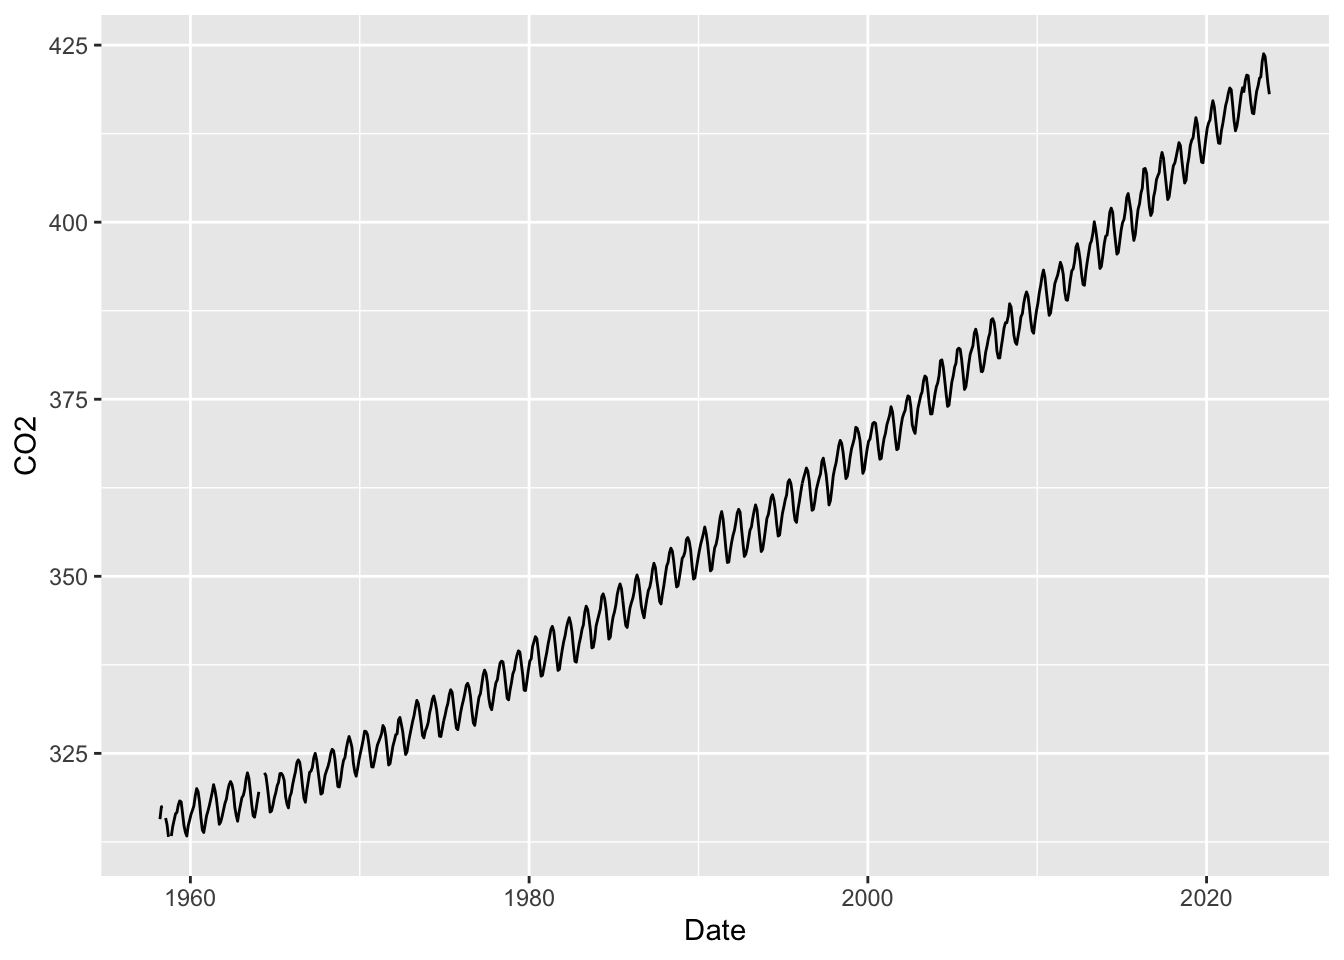
\includegraphics[width=0.49\linewidth]{book_files/figure-latex/global_warming-1} 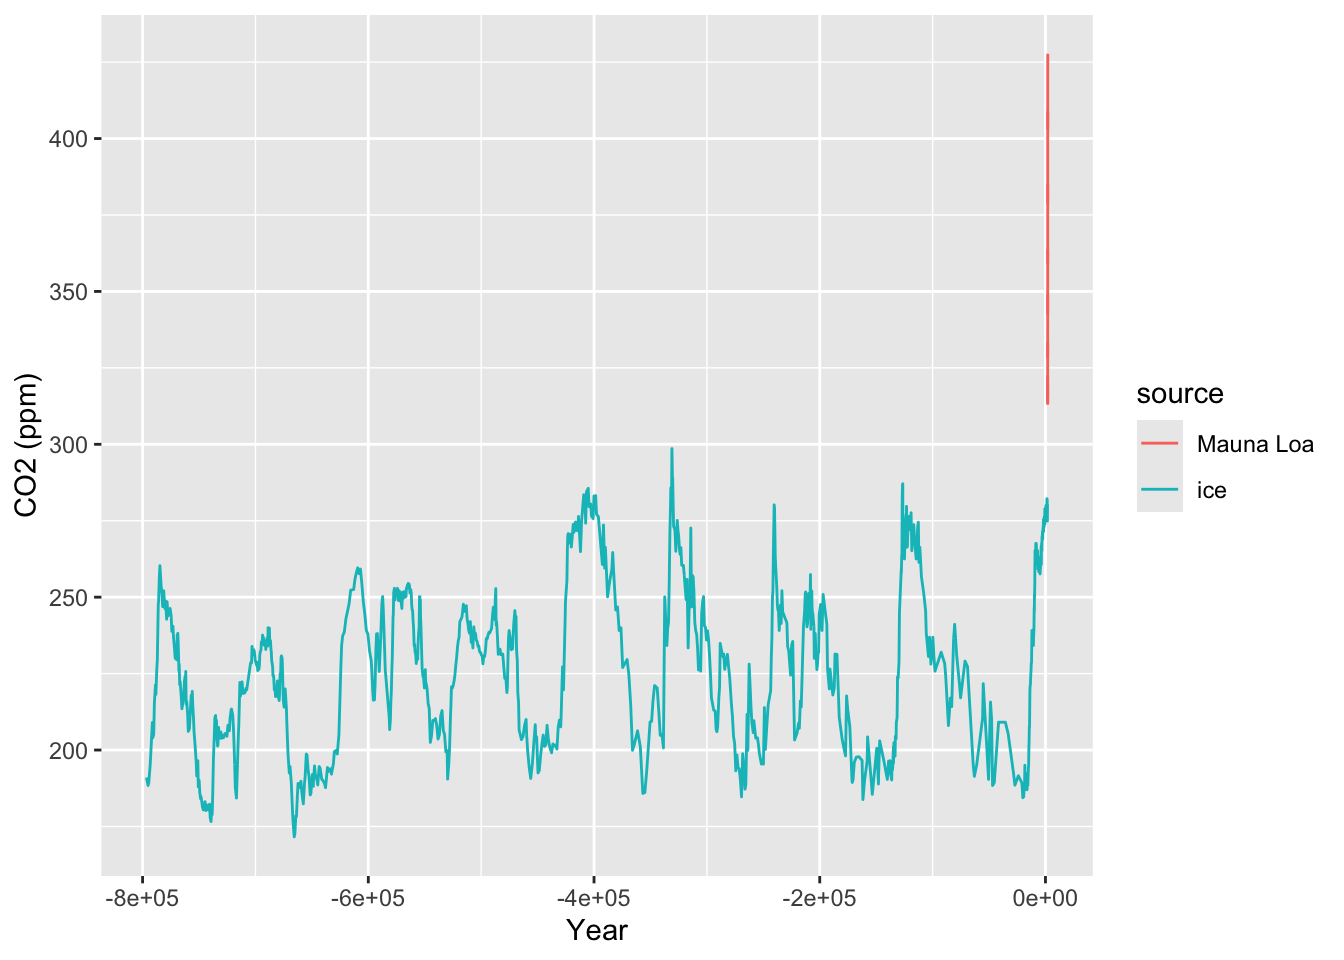
\includegraphics[width=0.49\linewidth]{book_files/figure-latex/global_warming-2}

This time series makes it clear that there has been a steady rise in atmospheric CO2 over the entire period of monitoring. The implications of this become startling when we compare the series to data which indicate the levels of CO2 which correspond to earlier historical times. This can be done by measuring the CO2 content of air trapped in ice cores. Careful analysis of the ice layers allow the identification of the time scale, which stretches back over hundreds of thousands of years. The CO2 measurements from ice cores has been superimposed on the plot of the Mauna Loa data in the right hand panel above. This makes it clear that the modern measurements of CO2 are `off the scale' of the historical levels.

In order to assuage any concerns about the comparability between the modern atmospheric and historical ice core CO2 measurements, the plots below focus on the period where these overlap. The left hand plot highlights the sudden dramatic rise in CO2 as the industrial revolution gathered pace. The right hand panel zooms in on the years when both types of measurement are available, indicating the very strong level of agreement between the two.

We will look at corresponding temperature changes later, but these data already paint a stark picture of the nature and size of the challenge we face in addressing climate change. The Intergovernmental Panel on Climate Change synthesises our scientific understanding of the process and continues to \href{https://www.ipcc.ch/2021/08/09/ar6-wg1-20210809-pr/}{report} on the current situation, with urgent calls to action.

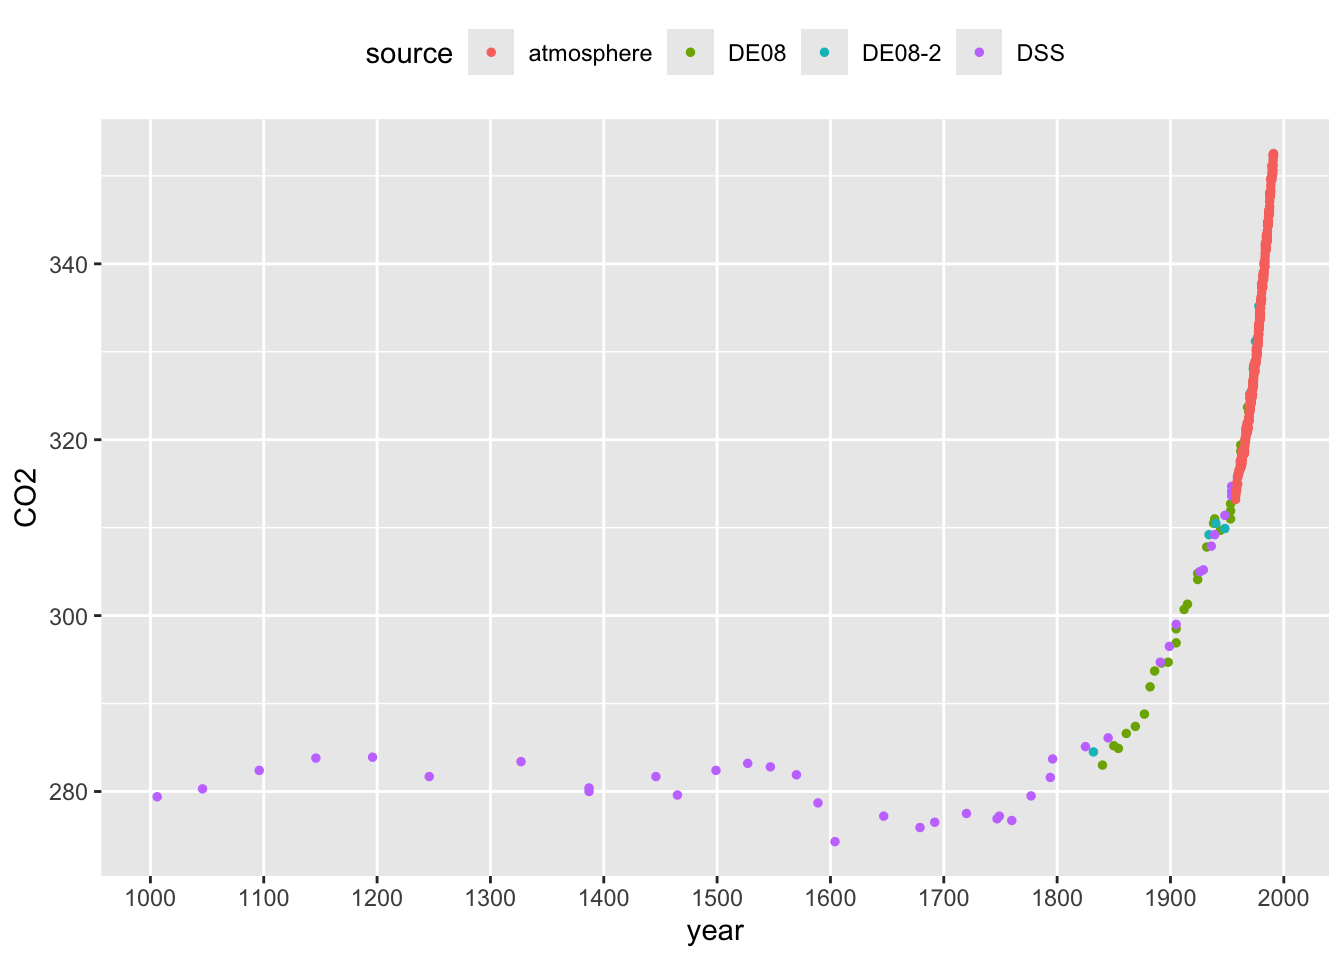
\includegraphics[width=0.49\linewidth]{book_files/figure-latex/law_dome-1} 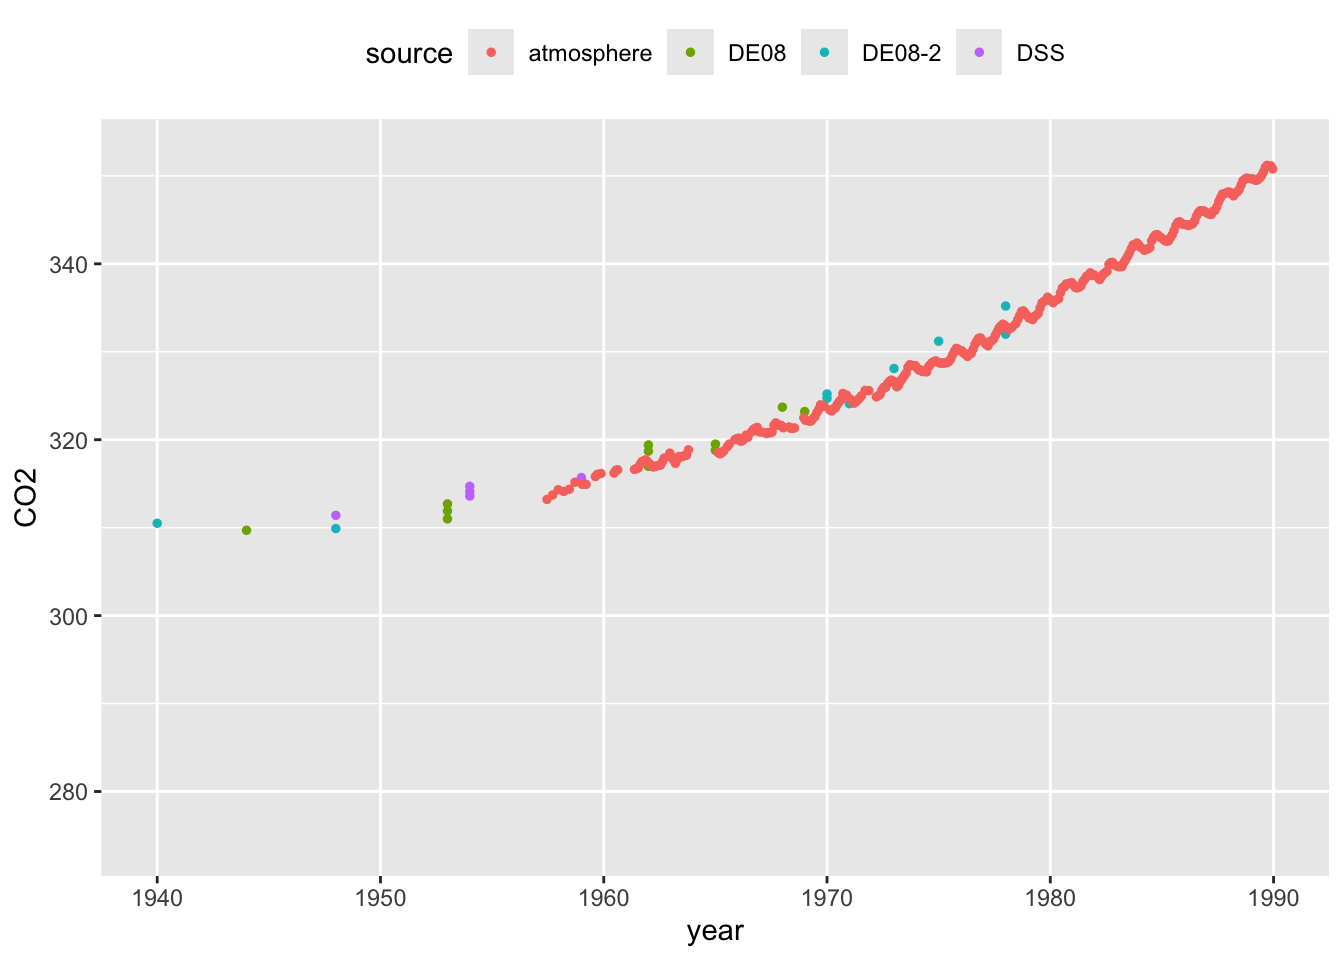
\includegraphics[width=0.49\linewidth]{book_files/figure-latex/law_dome-2}

This example highlights that, in some settings, there is a need for an appropriate \emph{control} to enable informative comparisons. Controls can sometimes be difficult to identify. In this case, considerable effort has been undertaken to ensure the validity of comparisons with the control data. The example also highlights the relevance of our scientific understanding of the context in which the experiment takes place. The physics of greenhouse gasses is well understood and this allows us to strengthen the interpretation of what we see in the data.

\subsection{The first tuberculosis trial}\label{the-first-tuberculosis-trial}

One of the very earliest systematic evaluations of medical treatment, marking a significant step in what we now term `clinical trials', was a study on the effects of \emph{Streptomycin} on pulmonary tuberculosis by Marshall et al. (\citeproc{ref-marshall_1948_bmj}{1948}).

The statistician Austin Bradford Hill, whose picture is below, introduced very important methodology in this study. In his \href{https://www.ncbi.nlm.nih.gov/pmc/articles/PMC3149409/}{review} of the development of clinical trials, Bhatt (\citeproc{ref-bhatt_2010_perspclinres}{2010}) writes ``This trial was a model of meticulousness in design and implementation, with systematic enrolment criteria and data collection compared with the ad hoc nature of other contemporary research. A key advantage of Dr Hill's randomization scheme over alternation procedure was ``allocation concealment'' at the time patients were enrolled in the trial. Another significant feature of the trial was the use of objective measures such as interpretation of x-rays by experts who were blinded to the patient's treatment assignment.''

\begin{figure}

{\centering 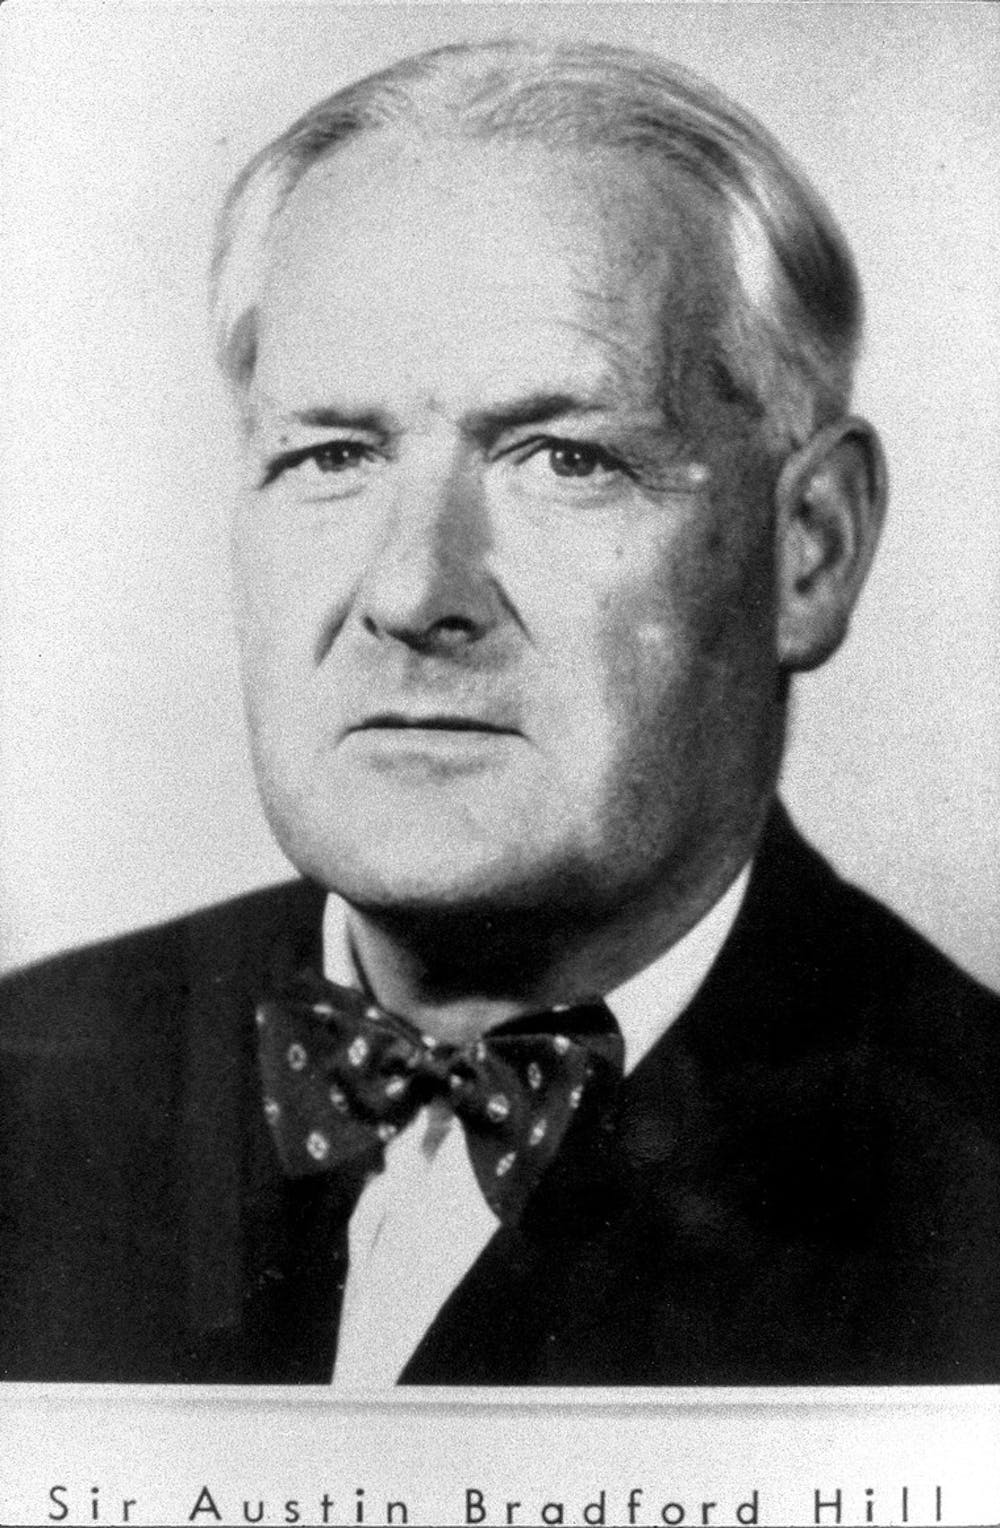
\includegraphics[width=0.2\linewidth]{images/bradford-hill} 

}

\caption{Sir Austin Bradford Hill,  Wellcome Collection, CC BY.}\label{fig:bradford-hill-image}
\end{figure}

The headline results reported in the \href{https://www.ncbi.nlm.nih.gov/pmc/articles/PMC2091872/pdf/brmedj03701-0007.pdf}{scientific paper} are shown in the table below.

\begin{tabular}{l|r|r}
\hline
Radiological assessment & Streptomycin group & Control group\\
\hline
Considerable improvement & 28 & 4\\
\hline
Moderate or slight improvement & 10 & 13\\
\hline
No material change & 2 & 3\\
\hline
Moderate or slight deterioration & 5 & 12\\
\hline
Considerable deterioration & 6 & 6\\
\hline
Deaths & 4 & 14\\
\hline
**Total** & **55** & **52**\\
\hline
\end{tabular}

The beneficial effects of the treatment are clear and we can have confidence in the conclusion because of the careful conduct of the trial. Key features of the design include the presence of a \emph{control} group and the use of randomisation.

\subsection{The birds and the bees: how to tell the sex of a herring gull}\label{the-birds-and-the-bees-how-to-tell-the-sex-of-a-herring-gull}

Herring gulls are found across the coastal regions of North-Western Europe. When studying the behaviour of these birds, it is useful to be able to identify sex. With this species, this is not possible by visual examination of the obvious anatomical features as the appropriate organs are internal. It would therefore be very useful to be able to identify the sex of a bird by taking simple measurements of some kind, on the assumption that the sexes are lijkely to differn in size, as happens with many animal species. The correct identification of the sex of a herring gull has to be carried out by dissection. The most suitable source of data for this purpose is therefore birds which have been found dead or have been culled for other reasons. Measurements from a sample of 100 male and 100 female birds, kindly provided by Prof.~Pat Monaghan from thte University of Glasgow, are available for investigation.

\begin{center}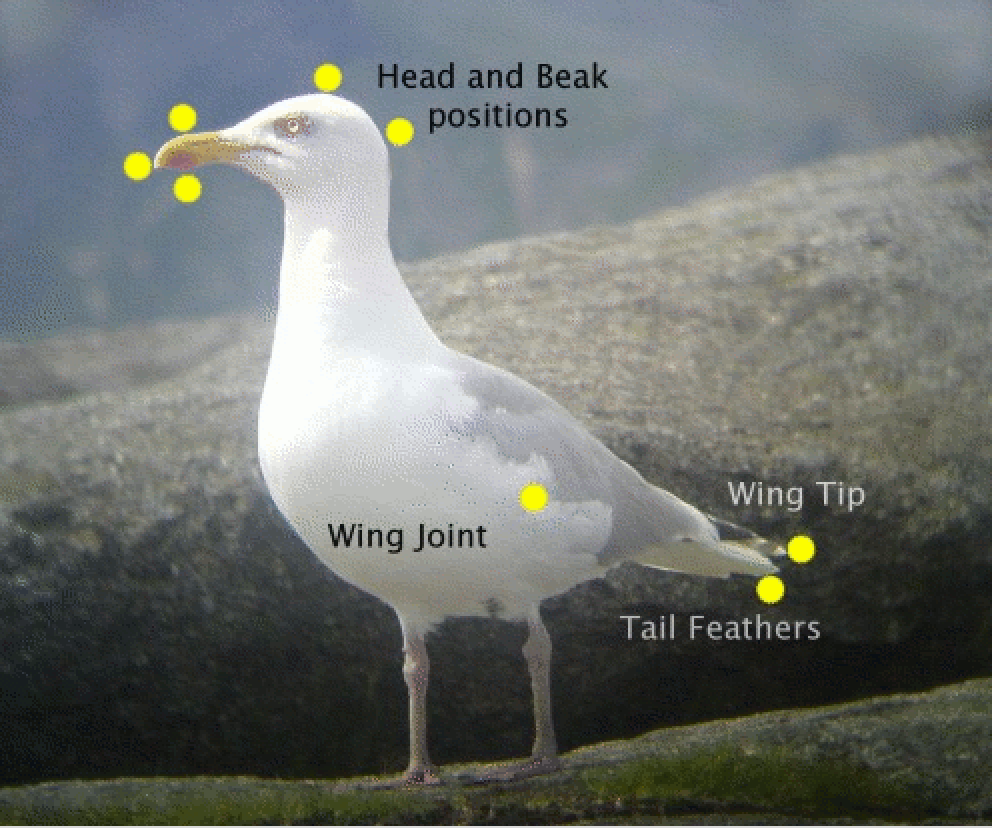
\includegraphics[width=0.5\linewidth]{images/herring-gull} \end{center}

Length measurements, based on the distance between two of the yellow landmarks in the picture above, could be useful in distinguishing between the sexes. as males and females tend to have different sizes in many species. There is an interactive application in R which can help in thinking this through. A gentle introduction to R is provided in Chapter \ref{R-introduction} but, if you have followed the guidance at the start of the book on installing R and the add-on package \texttt{rpanel}, then type in the following instructions into the \emph{console} window to launch the app.

\begin{Shaded}
\begin{Highlighting}[]
\FunctionTok{library}\NormalTok{(rpanel)}
\FunctionTok{rp.gulls}\NormalTok{()}
\end{Highlighting}
\end{Shaded}

Consider which pairs of landmarks might provide a suitable length measurement. Suitable criteria are:

\begin{itemize}
\tightlist
\item
  \emph{reproducible}, by yourself and others;
\item
  \emph{valid}, in what they aim to measure;
\item
  \emph{informative}, as they are likely to be different for male and females;
\item
  \emph{well calibrated}, as they target a feature of interest;
\item
  \emph{practical}, as measurements can be made reasonably easily.
\end{itemize}

Click on your selected pairs of landmarks and some feedback will be given. If you are able to identify some suitable measurements, checkboxes and buttons will appear to allow you to see some plots of the data, separated out by sex.

\subsection{Tracking the covid pandemic}\label{tracking-the-covid-pandemic}

When the covid19 pandemic began there was immediate and urgent effort to track its progress. That happened in many ways, most immediately in the numbers of deaths and hospital admissions. In the UK, when tests became available, the number of positive results was also regularly reported. The symptoms data collected by the app from the \href{https://health-study.zoe.com/data}{ZOE Health Study} provided another source of information.

Although these sources provided useful information, the most reliable estimates of covid infection levels came from a large survey conducted by the Office of National Statistics (ONS), in partnership with the University of Oxford, the University of Manchester, the UK Health Security Agency (UKHSA) and the Wellcome Trust. Swab and blood samples were provided by thousands of people from across the UK who had been selected and random and who had agreed to participate by providing repeated samples over an extended time period. Statistical modeling was also undertaken to ensure that the results represented the population as a whole.

The ONS provided extensive \href{https://www.ons.gov.uk/peoplepopulationandcommunity/healthandsocialcare/conditionsanddiseases/bulletins/coronaviruscovid19infectionsurveypilot/24march2023}{information} about the data, including details of the \href{https://www.ons.gov.uk/peoplepopulationandcommunity/healthandsocialcare/conditionsanddiseases/methodologies/covid19infectionsurveypilotmethodsandfurtherinformation}{methods and study design}. Scientific publication of the methods appeared in a \href{https://doi.org/10.1016/S2468-2667(20)30282-6}{\emph{Lancet} paper}. This is an example where very considerable effort was made to ensure that what we observe is an accurate representation of what is happening.

\begin{center}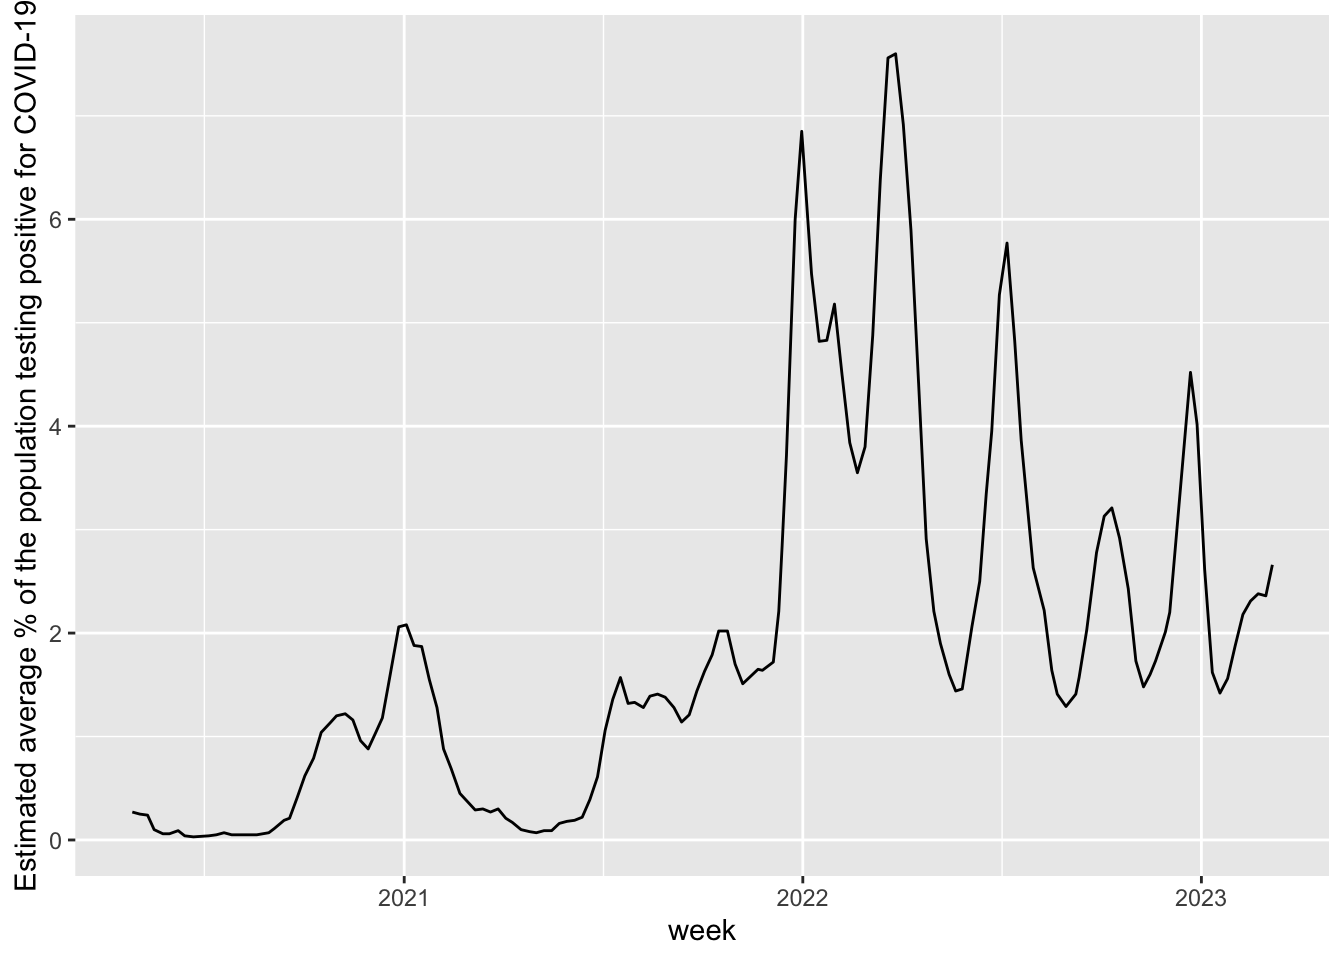
\includegraphics[width=0.7\linewidth]{book_files/figure-latex/covid_ons_survey-1} \end{center}

The plot above uses the survey data to track the pandemic in terms of the percentage of people in the UK who tested positive. The virulence of the infection changed over time so deaths and hospital admissions show rather different patterns. We will look at data on those later.

An account of the covid-19 tracking project is given in an \href{https://rss.org.uk/policy-campaigns/policy-groups/statistics-under-pressure-steering-group/statistics-under-pressure-informing-decision-makin/statistics-under-pressure-case-studies/how-do-we-know-how-many-people-have-covid-19-the-c/}{article} published by the Royal Statistical Society in its \emph{Statistics Under Pressure} series.
The hugely valuable nature of the information provided by the ONS survey is discussed in a \href{https://theconversation.com/the-ons-has-published-its-final-covid-infection-survey-heres-why-its-been-such-a-valuable-resource-202589?utm_medium=email&utm_campaign=Latest\%20from\%20The\%20Conversation\%20for\%20March\%2030\%202023\%20-\%202584725991&utm_content=Latest\%20from\%20The\%20Conversation\%20for\%20March\%2030\%202023\%20-\%202584725991+CID_f84345cb33348a28f83cffbda29f758a&utm_source=campaign_monitor_uk&utm_term=The\%20ONS\%20has\%20published\%20its\%20final\%20COVID\%20infection\%20survey\%20\%20heres\%20why\%20its\%20been\%20such\%20a\%20valuable\%20resource}{\emph{Conversation} article}.

\subsection{More complex data objects}\label{more-complex-data-objects}

The examples above mostly involve measurements of a single quantity of interest, such as CO\(_2\), the level of health improvement or the proportion of people with covid19. The herring gulls example might involve several different measurements on each bird. However, data can be much more complex. Some examples are:

\begin{itemize}
\tightlist
\item
  high-resolution images captured from a video camera monitoring wildlife movement;
\item
  free-form text entered into the search box of a web browser;
\item
  an extensive set of responses recorded from an individual in a survey, including later questions which are conditional on the responses to earlier questions;
\item
  a network describing the interactions of one individual with others in a group;
\item
  the life history of a hospital patient.
\end{itemize}

As the complexity of data increases, so the models required for analysis may also need to increase in sophistication. Nonetheless, some basic principles and concepts still apply and it is the aim of this book to discuss these. While the focus is on relatively straightforward types of data, the ideas will provide helpful building blocks for more complex situations.

\section{Some broad issues}\label{some-broad-issues}

It is worthwhile reflecting on some of the broad issues which have already arisen in our review of these examples of data. To structure our reflections it will be helpful to recall the PPDAC framework discussed in the Preface, displayed below in graphical form. In this section we will focus on the \emph{Problem}, \emph{Plan} and \emph{Data} stages.

\begin{center}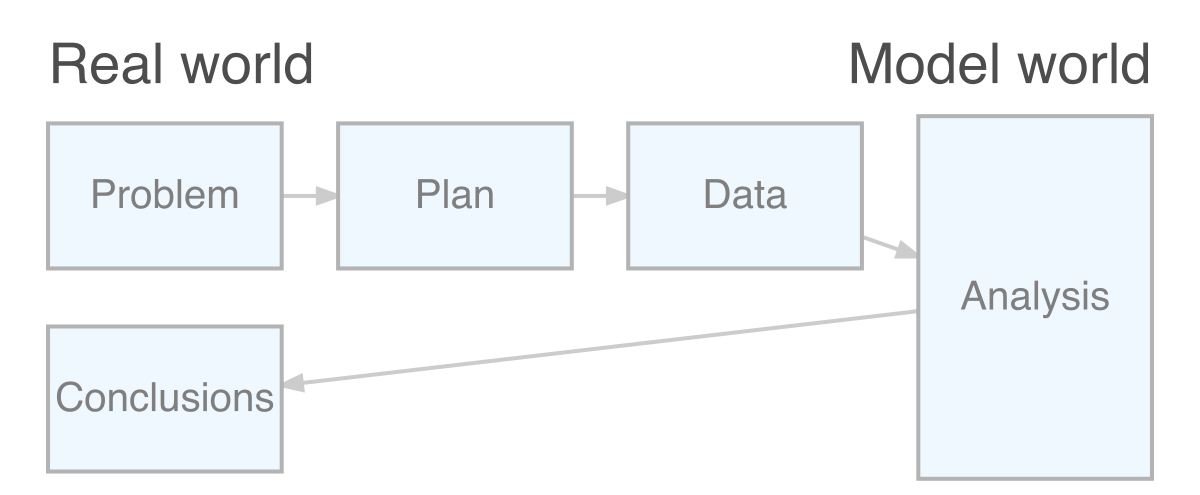
\includegraphics[width=0.7\linewidth]{images/ppdac_1} \end{center}

\subsection{What's the problem?}\label{whats-the-problem}

It is very important to define the objectives of an experiment clearly. Failure to do this will make subsequent analysis and interpretation very difficult. Pilot studies are a perfectly valid preliminary step but a clear objective is still needed. `Fishing expeditions' are of rather limited use.

Our objectives will be informed by previous work so a review of the scientific literature is a wise start. Scientific knowledge of the subject domain will be very helpful not only in deciding what problem to tackle but also in informing later decisions in the planning process and in due course in interpreting the results of our analysis.

There are some general aspects of this process which are worth highlighting. The first is the distinction between an \emph{observational study} where we simply observe and record variables of interest. We do not intervene or influence the situation in any way other by recording what we see. In an observational study we can only identify \emph{association} between variables. A simple of example is the association between social or economic characteristics and political voting patterns.

In contrast, a \emph{designed experiment} involves the specification of `treatments' which are assigned by the experimenter. Rather than simply observe, we intervene. We are then interested in the way the treatments affect the outcome. If a designed experiment is conducted well it allows us to identify \emph{causal} relationships between variables. A simple example is a clinical trial, such as the tuberculosis trial described in Section \ref{examples-data}, where we compare the effects of different treatments on the recovery of patients suffering from a particular medical condition.

A second general issue is whether our aim is to \emph{understand} the processes at work in our scientific context or whether we simply want to \emph{predict} an outcome or design a system which will \emph{classify} future observations into different groups. The classification of herring gulls into male and female groups discussed in Section \ref{examples-data} is an example of the latter. This is a case where we may not be primarily interested in which variables are involved in our model, simply in how successful our model is in prediction or classification. This may change our attitude to building a model, when the time comes, but it is also helpful to be aware of the distinction between these two aims from the start of the planning process.

\subsection{What's the plan?}\label{whats-the-plan}

Acquiring data which are appropriate, informative and unbiase requires careful thought. The ONS covid-19 survey was described in Section \ref{where-data}. Take a look at the \href{https://www.ons.gov.uk/peoplepopulationandcommunity/healthandsocialcare/conditionsanddiseases/methodologies/covid19infectionsurveypilotmethodsandfurtherinformation}{methodology guide} for this survey. It is very extensive, covering all the major issues which had to be considered.

One of the exercises at the end of this chapter ask you to consider how you might design a simple experiment to investigate the operation of short term memory, known to psychologists as ``working memory''. How is a list of items recalled from memory? This is an experiment which can be caried out in a classroom or small group setting. It might surprise you just how extensive the list of detailed arrangements needs to be.

One of the important tasks is to identify which measurements should be taken. The list should include not only those which are mentioned in the definition of the problem being tackled but also those which we know or suspect from previous work or our scientific understanding are likely to influence the process we are studying. This will help us to consider an appropriate experimental design - a topic we will revisit in a later chapter.

\subsection{Where do the data come from?}\label{where-data-subsection}

The diagram at the start of this section includes two headings, ``Real world'' and ``Model world''. The question our experiment aims to tackle is about what is going on ``out there in the wild'', even when the ``wild'' refers to a laboratory setting. If we consider all the observations we might ever make then we can view this as the \emph{population} we are studying. The process of collecting a particular dataset then delivers a \emph{sample}. Our modelling process will use this sample to try to understand what is going on in the population. It is then crucially important to obtain a sample which properly represents the population and does not suffer from serious \emph{bias}. If we make serious mistakes at this stage, it is unlikely that we will be able to retrieve the situation.

A good mechanism for avoiding bias is to use \emph{randomisation}. This applies in two ways. The first is to the process of identifying which items from the population are recruited into our sample, ideally ensuring that all potential items have an equal chance of appearing. The second applies to the allocation of any treatments to sampled items. The tuberculosis trial outlined in Section \ref{examples-data} is one of the first occasions where this was used. It is now a standard component of clinical trials worldwide.

\subsection{Who do you trust?}\label{who-do-you-trust}

We live in a world where `fake news' has become a commonly used term. Not everyone is careful in the way data are collected, analysed and interpreted. Sadly, data are sometimes used selectively to support a conclusion already adopted. It is very important that this is countered and that the analysis of data is conducted in an honest and professional manner.

The UK Statistics Authority is the body which oversees the production of official statistics in the UK. Its \href{https://code.statisticsauthority.gov.uk}{code of practice} is based on the principles of:

\begin{itemize}
\tightlist
\item
  \emph{trustworthiness}, confidence in the people and organisations that produce statistics and data;
\item
  \emph{quality}, data and methods that produce assured statistics;
\item
  \emph{value}, statistics that support society's needs for information.
\end{itemize}

The \href{https://code.statisticsauthority.gov.uk/wp-content/uploads/2022/05/Code-of-Practice-for-Statistics-REVISED.pdf}{full code} is well worth reading. Although it is couched in terms of official statistics, providing information for the public and for government, the principles it describes are very important. A \href{https://isi-web.org/declaration-professional-ethics}{Declaration on Professional Ethics} is also provided by the \emph{International Statistical Institute}.

In addition to the obligation on all who collect and analyse data to act with professionalism and integrity, specific ethical considerations arise in the planning and design of experiments, particularly those involving humans. Indeed, the protocol for any experiment involving humans must be approved by an appropriate ethical committee before it can be put into practice. A simple example is in a clinical trial to compare two treatments where the size of the sample must be considered very carefully. The sample must be large enough to enable a clear conclusion about the treatments to be reached, but if it is too large then some patients may end up being given a treatment which might clearly have been shown by a smaller trial to be inferior. That would not be ethical.

We will often find ourselves using data from other sources as part of our investigations. Indeed, many different sources are used in this book.
The issue of trustworthiness, raised in the UK Statistics Authority code of conduct, again arises. What sources can we trust as reliable?

Some guidance comes from the source organisations stated aims and code of conduct. Reputation also matters. Open documentation is important, so that the details of the data collection process can be reviewed. Accountability matters too, so that there is a mechanism for query and complaint if the need arises.

The RSS has provided a document, \href{https://rss.org.uk/RSS/media/File-library/Policy/2024/RSS-guide-to-statistics-on-social-media.pdf}{\emph{Sound or suspicious? Ten tips to be statistically savvy}} which offers advice on how to assess claims that are made.

\section{What could possibly go wrong?}\label{what-could-possibly-go-wrong}

It is very instructive to think about studies which went wrong.

\subsection{US presidential elections, 1936 and 1948}\label{us-presidential-elections-1936-and-1948}

The \emph{Literary Digest} was a magazine which surveyed 10 million people, beginning with its own readers, who they planned to vote for in the 1936 US presidential election. A massive 2.4 million people responded, leading to the prediction of a clear win for the candidate Alf Landon. In fact, Franklin Delano Roosevelt had a landslide victory. What went wrong?

For another occasion when things went wrong in the prediction of the outcome of a US presidential election, see the \href{https://www.latimes.com/archives/la-xpm-1998-nov-01-mn-38174-story.html}{article in the Los Angeles Times} about the 1948 election.

\section{Further reading}\label{further-reading}

The Royal Statistical Society has a very helpful \href{https://rss.org.uk/RSS/media/File-library/Policy/2025/RSS-CCTF-guide-to-UK-official-statistics-on-climate-change.pdf}{Guide to UK official statistics on climate change}.

The \href{https://archive.ceda.ac.uk}{CEDA Archive}, maintained by the National Environmental Research Council (NERC) in the UK, contains a very large collection of environmental data from atmospheric and earth observation research.

If data are to be collected through a survey, the nature and construction of the questions are very important, to avoid bias or leading the respondent. The Pew Research Centre, a high profile independent organisation, provides a helpful discussion of \href{https://www.pewresearch.org/our-methods/u-s-surveys/writing-survey-questions/}{writing survey questions}.

Copernicus: European environmental data.
\url{https://surfobs.climate.copernicus.eu/dataaccess/index.php}

Diggle and Chetwynd (\citeproc{ref-diggle_2011_book}{2011})

Rosling (\citeproc{ref-rosling_2018_book}{2018})

The Tiger That Isn't. Andrew Dilnot \& Michael Blastland.

How to lie with Statistics. Darrell Huff.

Damned Lies and Statistics. Joel BEst.

More Damned Lies and Statistics. Joel Best.

Innumeracy. John Allen Paulos.

Reckoning with Risk. Gerd Gegerenzer. (Some people object to technical errors?)

Dicing with Death. Stephen Senn.

Risk. John Adams.

Britain in Numbers. Simon Briscoe.

Why Do Buses Come in Threes. Rob Eastaway.

How Long is a Piece of String. Rob Eastaway.

How to Take a Penalty. Rob Eastaway.

\section{Exercises}\label{exercises}

\subsection{An investigation of short-term memory}\label{an-investigation-of-short-term-memory}

Consider how you might design a simple experiment to investigate the operation of short term memory, known to psychologists as ``working memory''? How is a list of items recalled from memory? This is an experiment which can be caried out in a classroom or small group setting. It might surprise you just how extensive the list of detailed arrangements needs to be.

Once you have spent some time considering this, you may like tyo consult Bowman (\citeproc{ref-bowman-1994-teachingstatistics}{1994}) which describes some of the issues which arose in a classroom setting.

\subsection{A survey of dental health}\label{a-survey-of-dental-health}

Imagine you have been commissioned to conduct a survey of the dental health of five year old children in England. Write down some of the things on which you will need to make decisions and sketch out some possible answers. This should include how a suitable sample of children will be selected, what measurements will be made, how this will be done, and another other issues which you think are relevant.

In fact, a survey of exactly this type is regularly conducted under the National Dental Epidemiology Programme (NDEP) for England. Once you have spent some time considering the issues, you can see the detail of what was done in the documents available \href{https://www.gov.uk/government/statistics/oral-health-survey-of-5-year-old-children-2017\#:~:text=The\%20results\%20of\%20the\%20oral,experience\%20of\%20obvious\%20dental\%20decay}{here} for the 2016-2017 survey. The \href{https://assets.publishing.service.gov.uk/government/uploads/system/uploads/attachment_data/file/774469/Oral_health_survey_protocol_5_year_olds_2016.pdf}{protocol document} describes the planning of the survey in considerable detail. The results of a further survey in 2022, using the same protocol, are also \href{https://www.gov.uk/government/statistics/oral-health-survey-of-5-year-old-children-2022}{available}.

\subsection{Hearings aid and dementia}\label{hearings-aid-and-dementia}

A \href{https://www.thelancet.com/journals/lanpub/article/PIIS2468-2667(23)00048-8/fulltext}{Lancet paper} studied the association between hearing loss and dementia, in particular examining the role of hearing aids. The interpretation of the findings were:

\begin{quote}
In people with hearing loss, hearing aid use is associated with a risk of dementia of a similar level to that of people without hearing loss. With the postulation that up to 8\% of dementia cases could be prevented with proper hearing loss management, our findings highlight the urgent need to take measures to address hearing loss to improve cognitive decline.
\end{quote}

Are there other possible interpretations? You may wish to look at \href{https://www.bgs.org.uk/blog/hearing-aid-use-reduces-dementia-or-is-it-dementia-reduces-hearing-aid-use-its-both}{this article} published by the British Geriatrics Society which discusses the issue. The article also provides a link to a further scientific paper for the technical detail.

\part{Statistical Inference}\label{part-statistical-inference}

\chapter{Inference: turning data into evidence}\label{inference}

So far we have considered how to read, organise and visualise datasets. We are now ready to discuss one of the main themes of statistics, namely weighing up the evidence for the presence or size of different features in the population lying behind the data. That process is referred to as \emph{statistical inference}. The first step in doing this is to think about the uncertainty or variation involved in the data and how to quantify this. That will enable us to discuss some standard tools, such as confidence intervals and hypothesis test, which we will explore in this chapter in some simple settings.

\section{Samples and populations}\label{samples-and-populations}

The distinction between a \emph{sample} of data and the \emph{population} from which the data come was mentioned briefly in Section \ref{where-data-subsection}, where a population was defined rather informally as the collection of all the observations we could ever make of the process we are studying. We will now explore this further by carrying out a kind of `thought experiment'. By sampling from a population whose characteristics are known, using R to do so, we can investigate how well the features of a sample guide us on the features of the underlying population.

To give our thought experiment a little context, let's assume we are taking water samples from a particular location on a river with a view to assessing the water quality. This is often quantified through the percentage of dissolved oxygen.

The \texttt{rp.sample} function in the \texttt{rpanel} package provides a convenient means of experimenting with this situation. The plots below give a flavour of what can be done but you may find it more instructive to run the function `live' to create your own images and experiment with different settings. The simple instruction \texttt{rp.sample()} will launch a window with a panel of interactive controls.

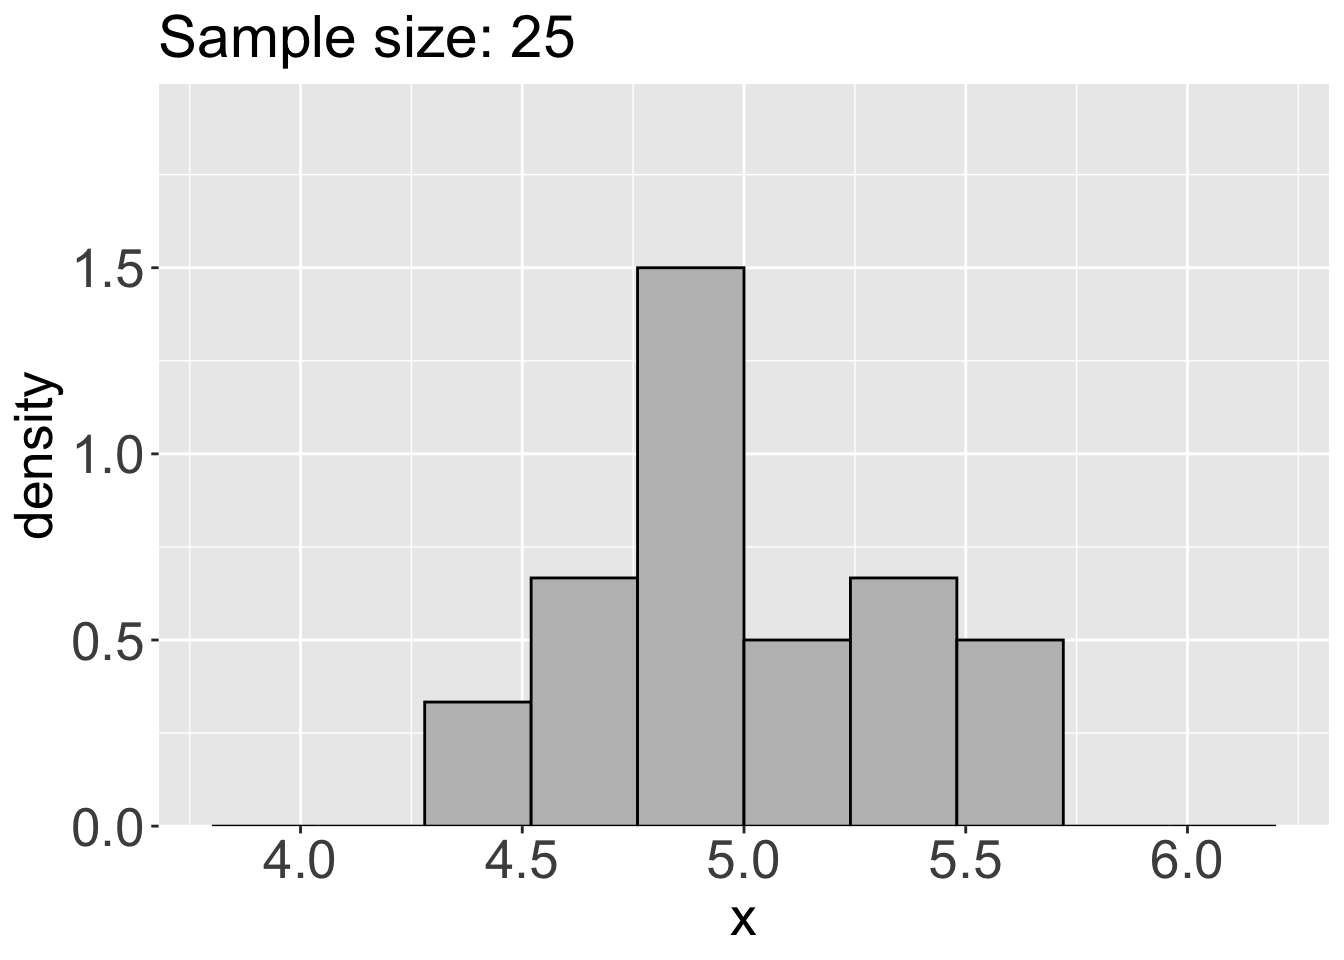
\includegraphics[width=0.24\linewidth]{book_files/figure-latex/rp_sample_population_plots-1} 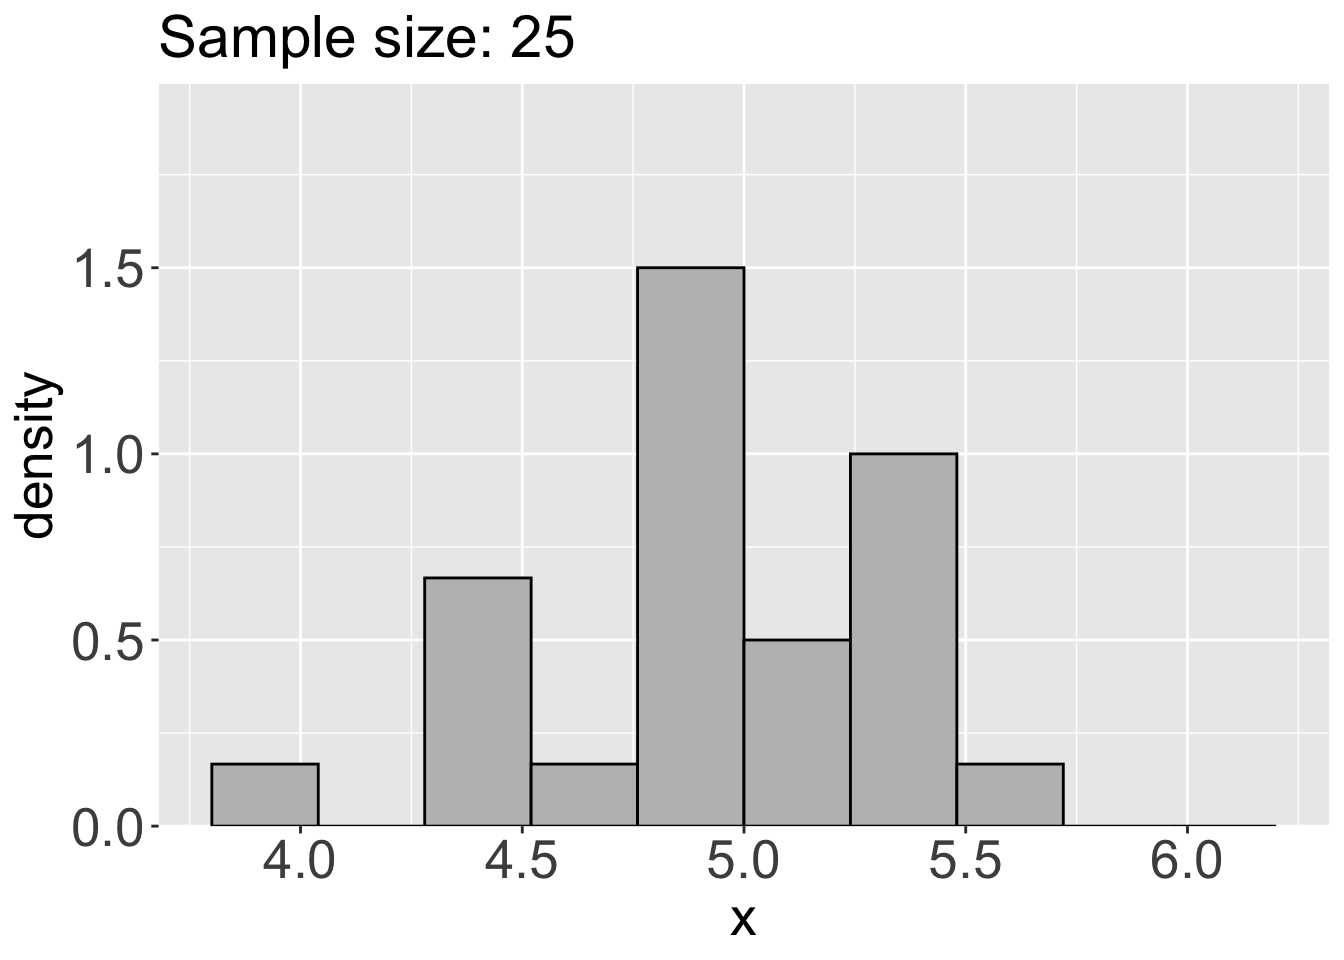
\includegraphics[width=0.24\linewidth]{book_files/figure-latex/rp_sample_population_plots-2} 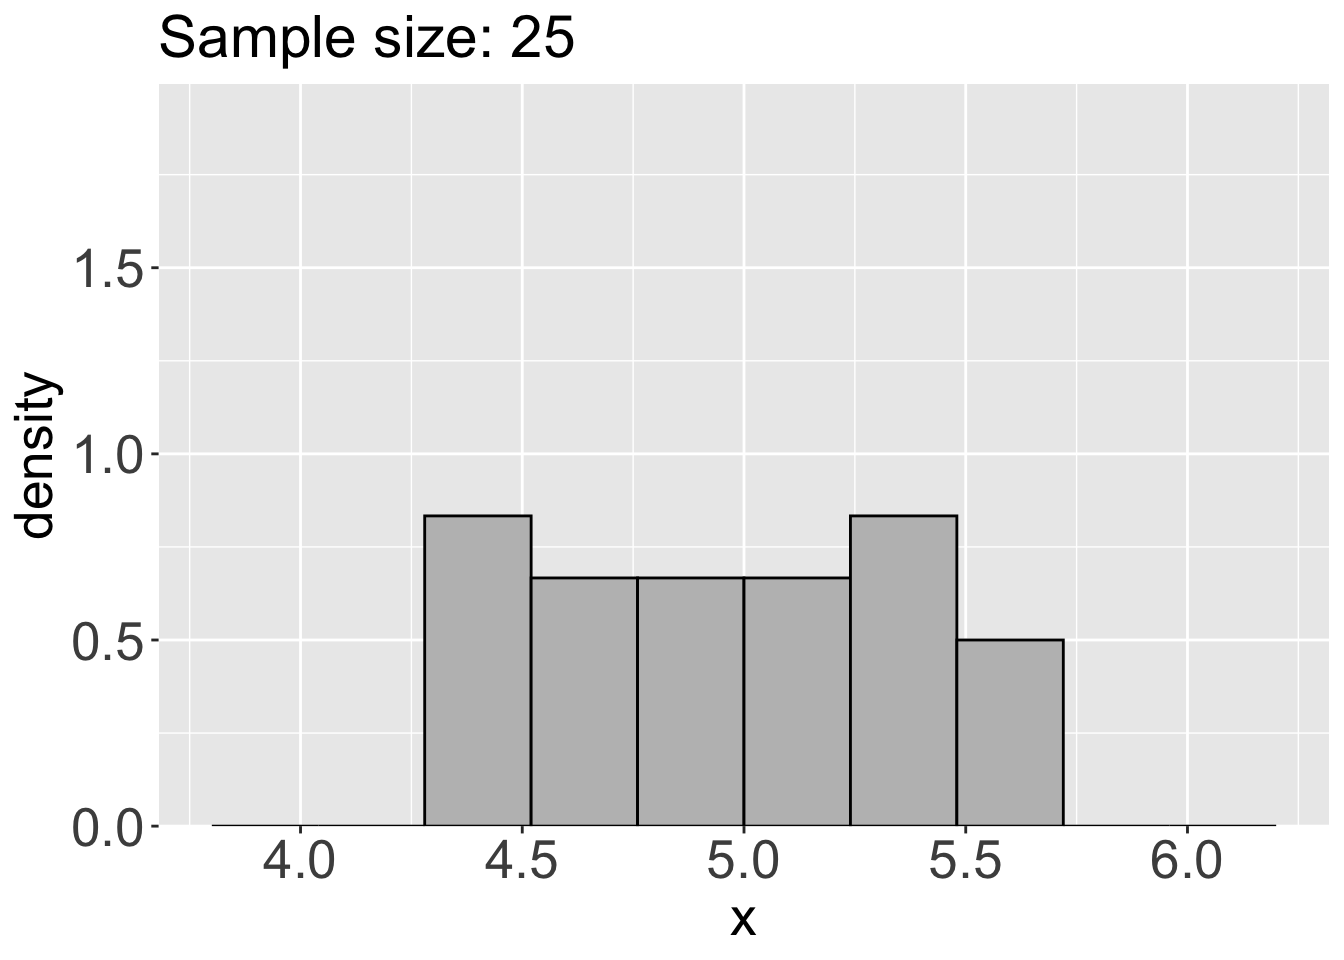
\includegraphics[width=0.24\linewidth]{book_files/figure-latex/rp_sample_population_plots-3} 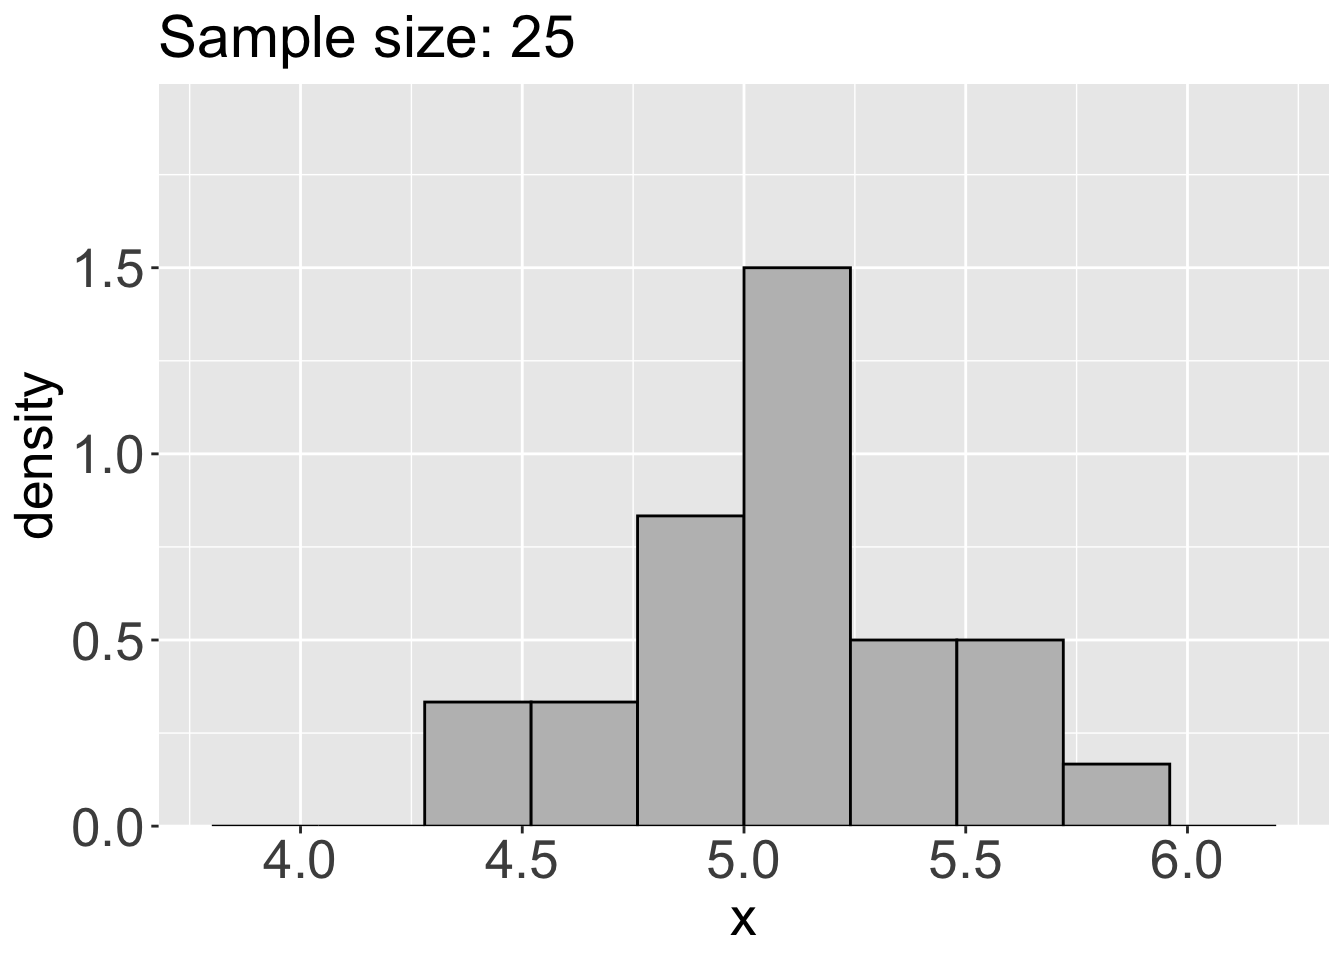
\includegraphics[width=0.24\linewidth]{book_files/figure-latex/rp_sample_population_plots-4} 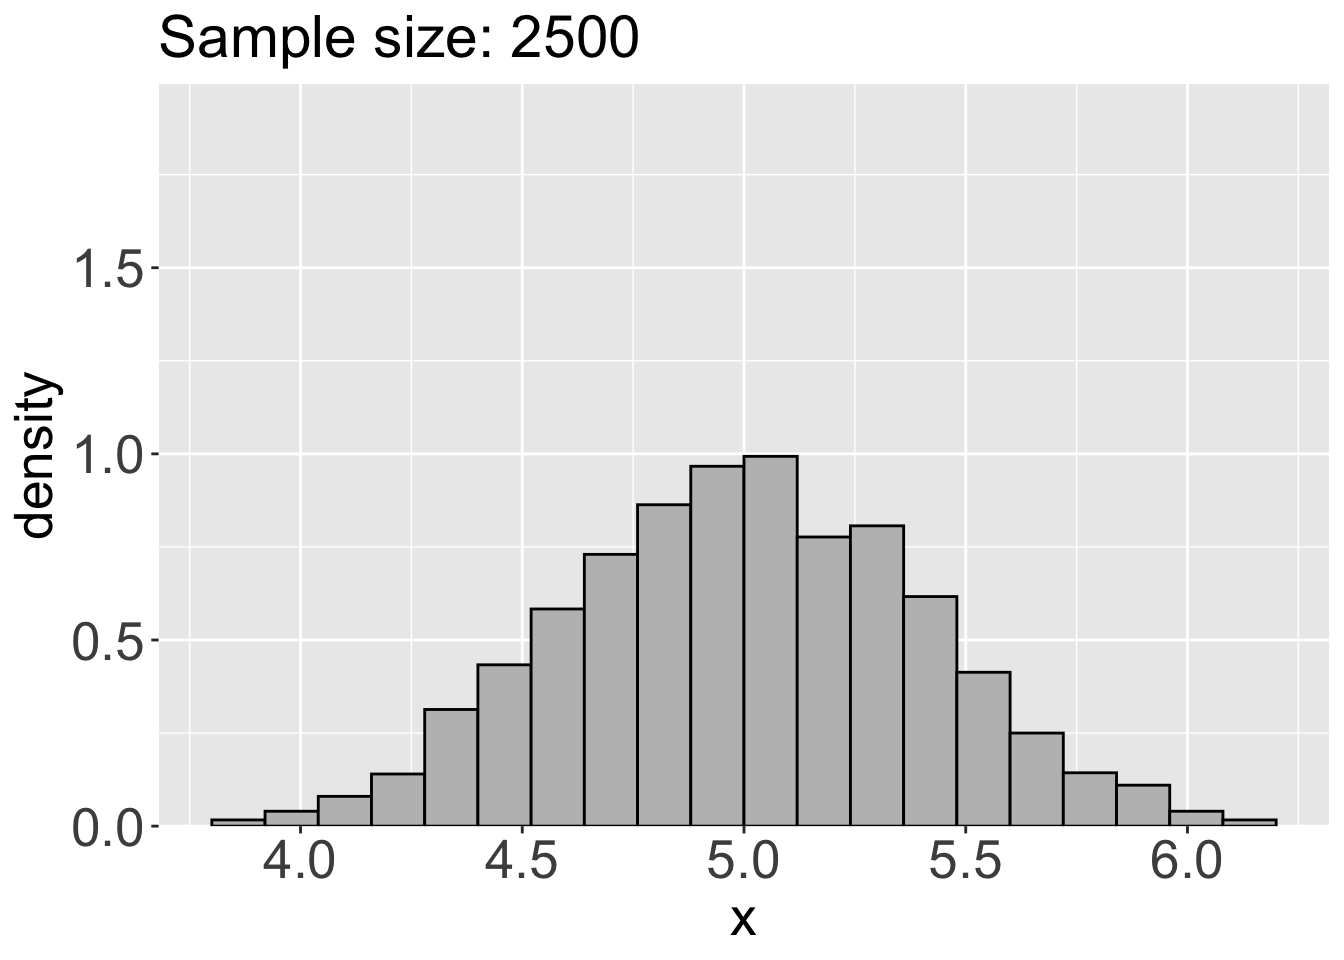
\includegraphics[width=0.24\linewidth]{book_files/figure-latex/rp_sample_population_plots-5} 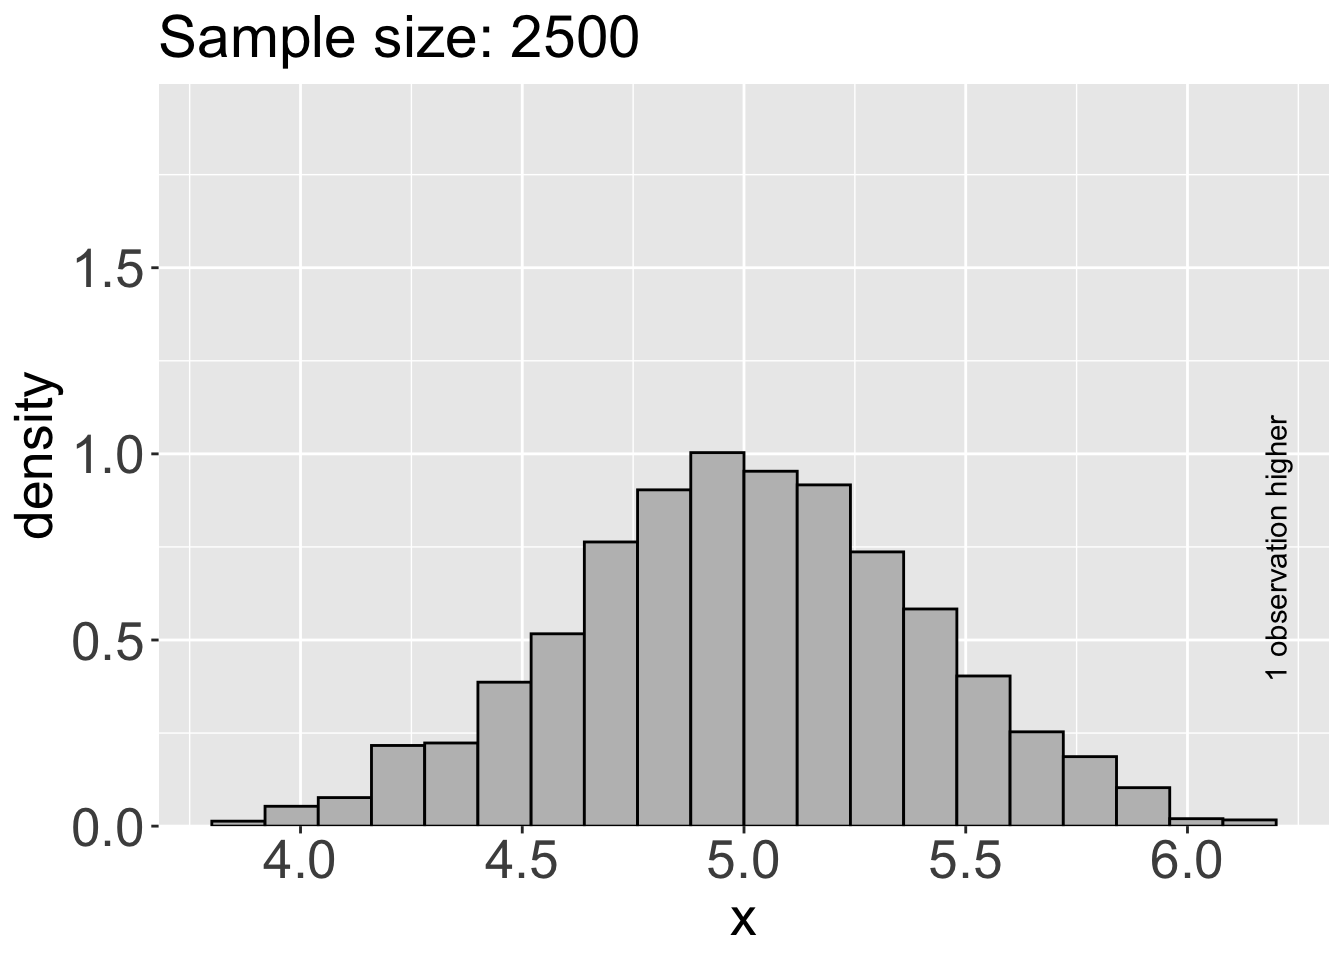
\includegraphics[width=0.24\linewidth]{book_files/figure-latex/rp_sample_population_plots-6} 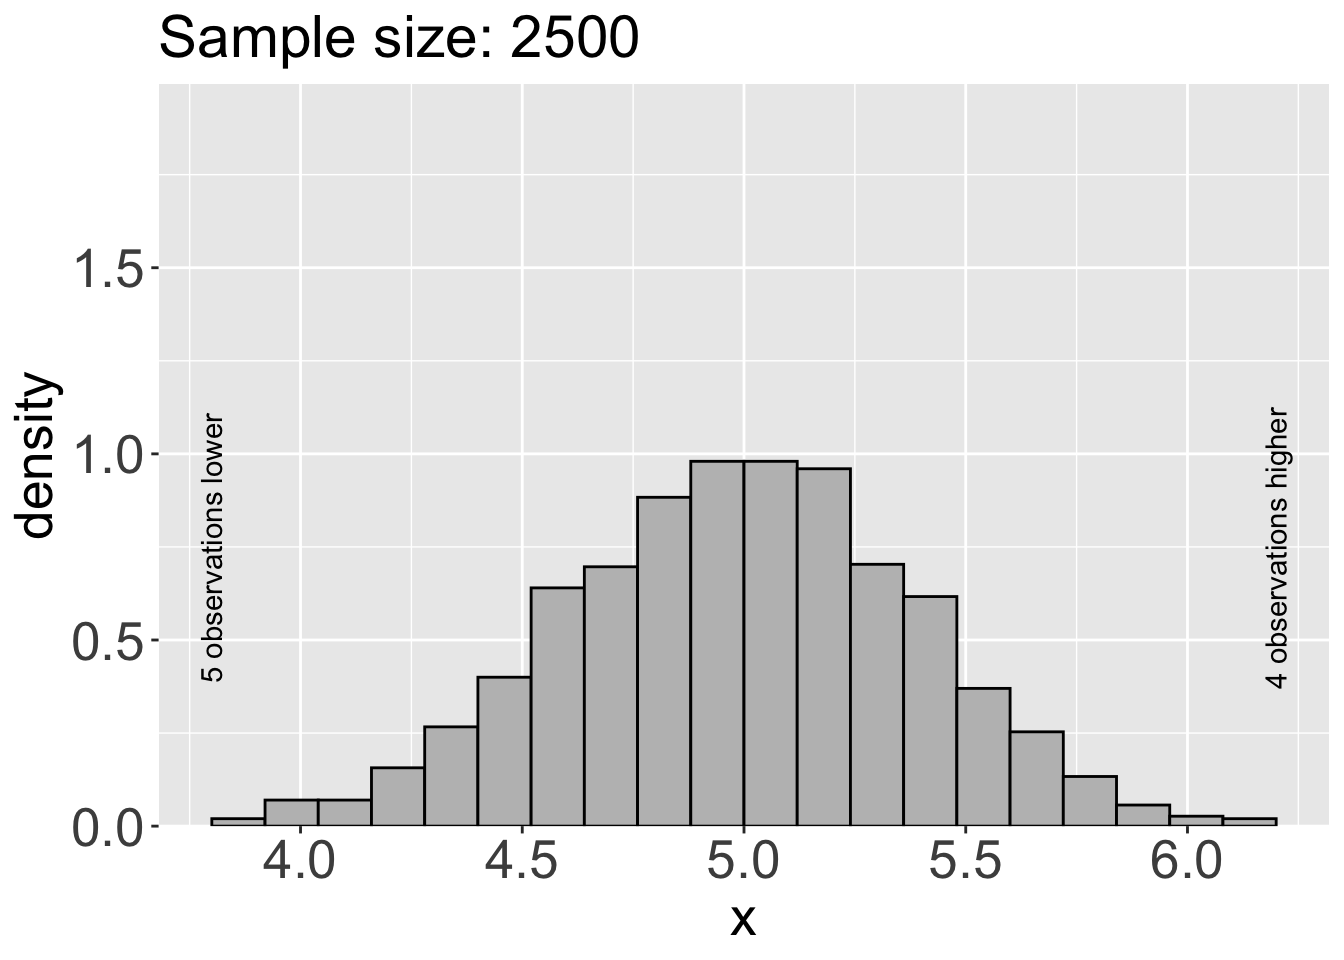
\includegraphics[width=0.24\linewidth]{book_files/figure-latex/rp_sample_population_plots-7} 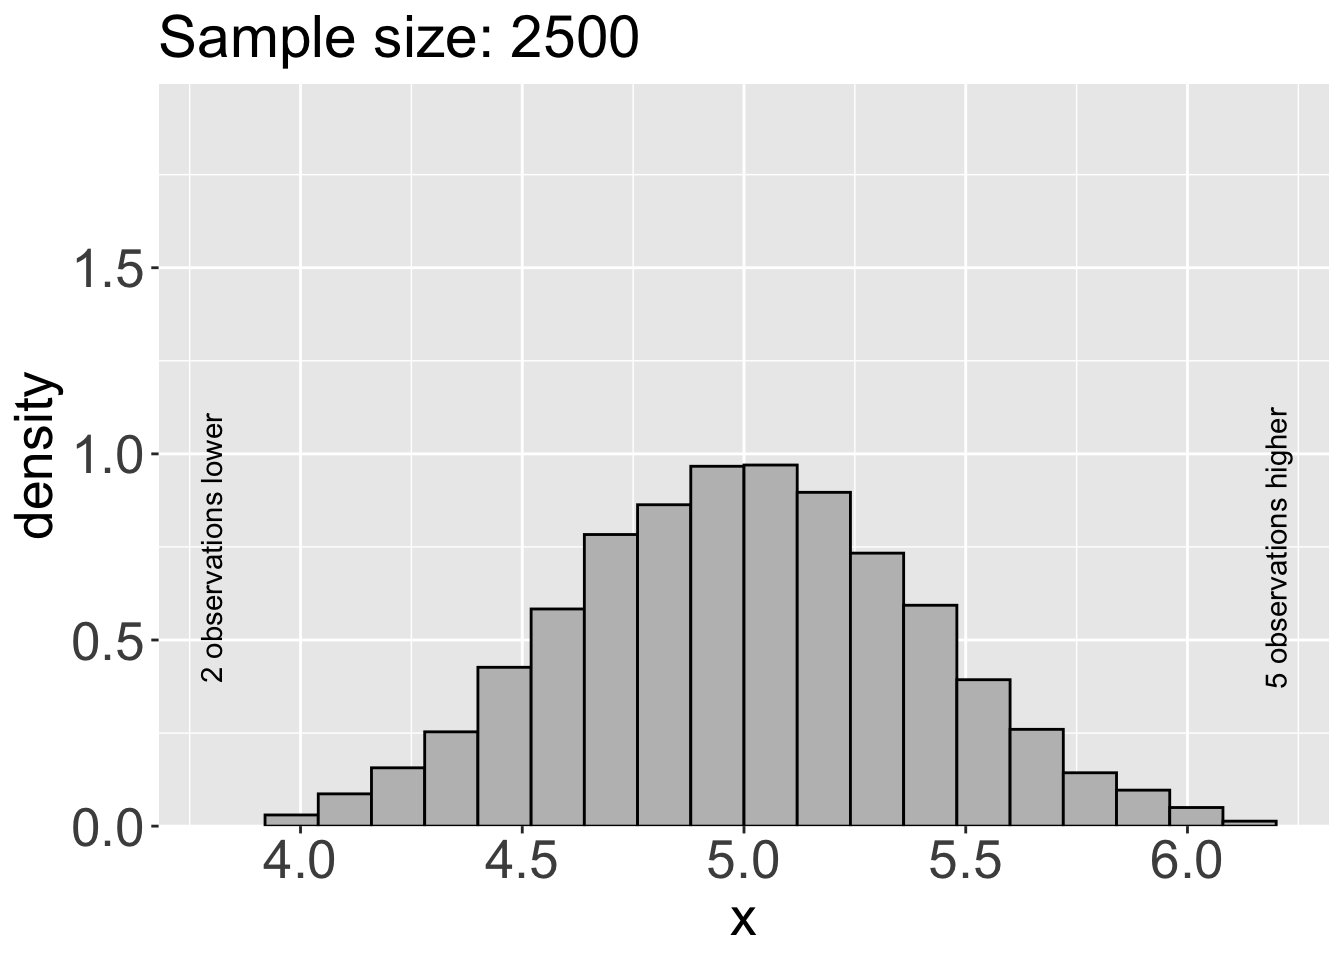
\includegraphics[width=0.24\linewidth]{book_files/figure-latex/rp_sample_population_plots-8} 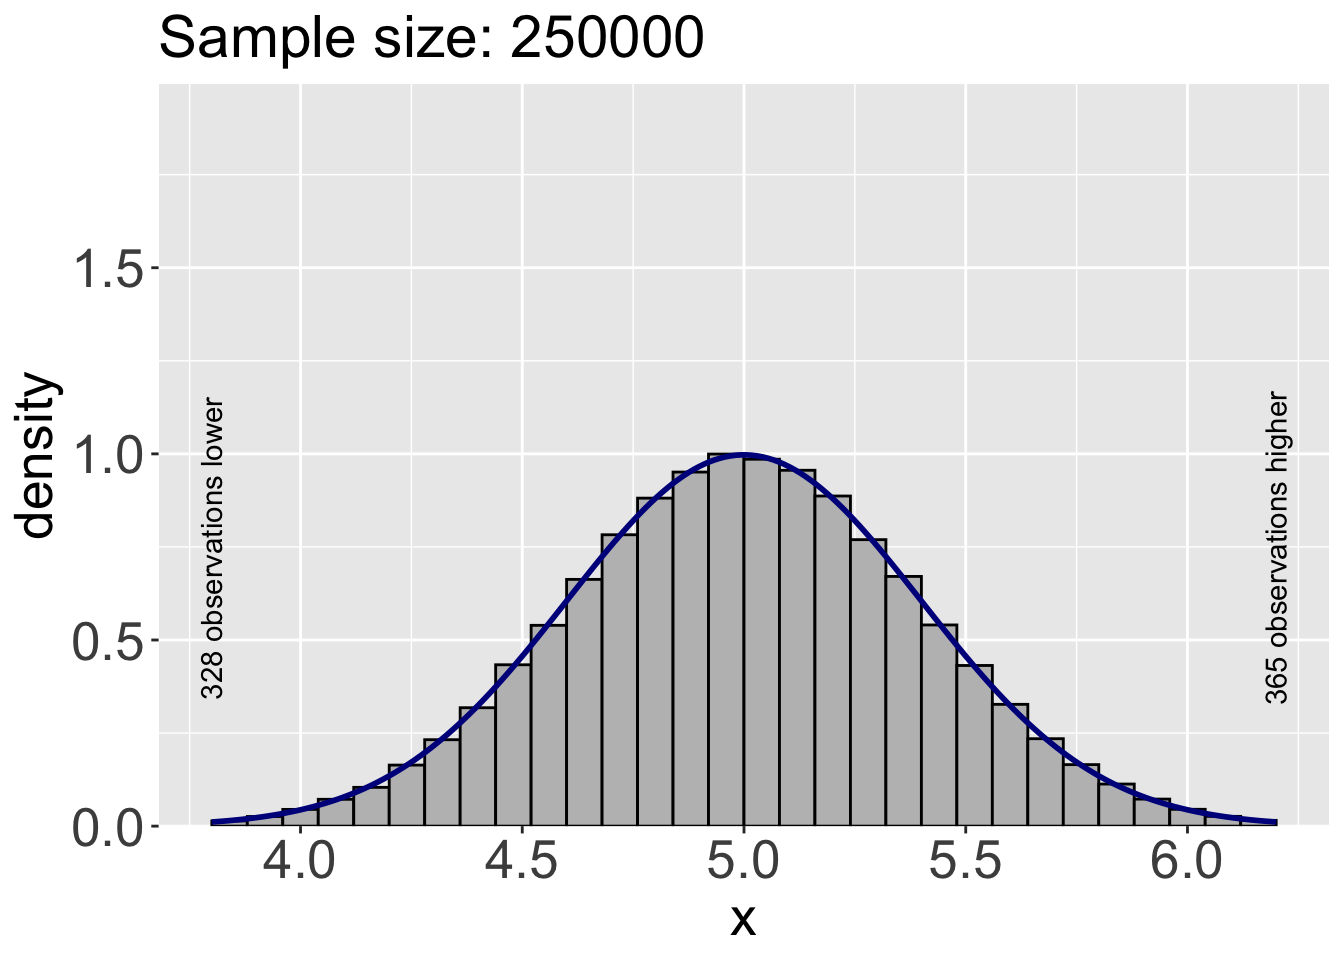
\includegraphics[width=0.24\linewidth]{book_files/figure-latex/rp_sample_population_plots-9} 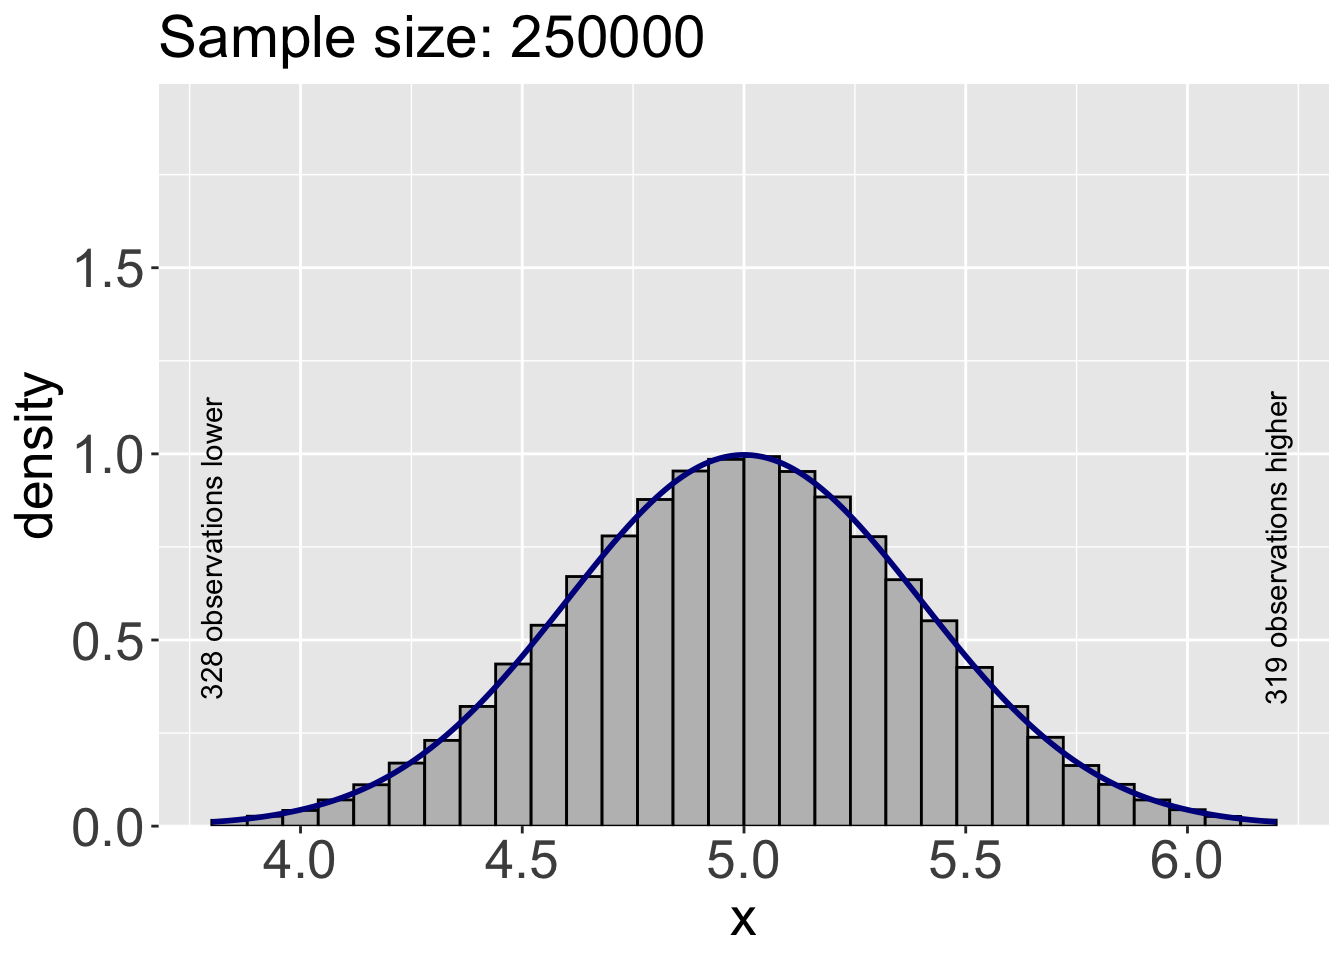
\includegraphics[width=0.24\linewidth]{book_files/figure-latex/rp_sample_population_plots-10} 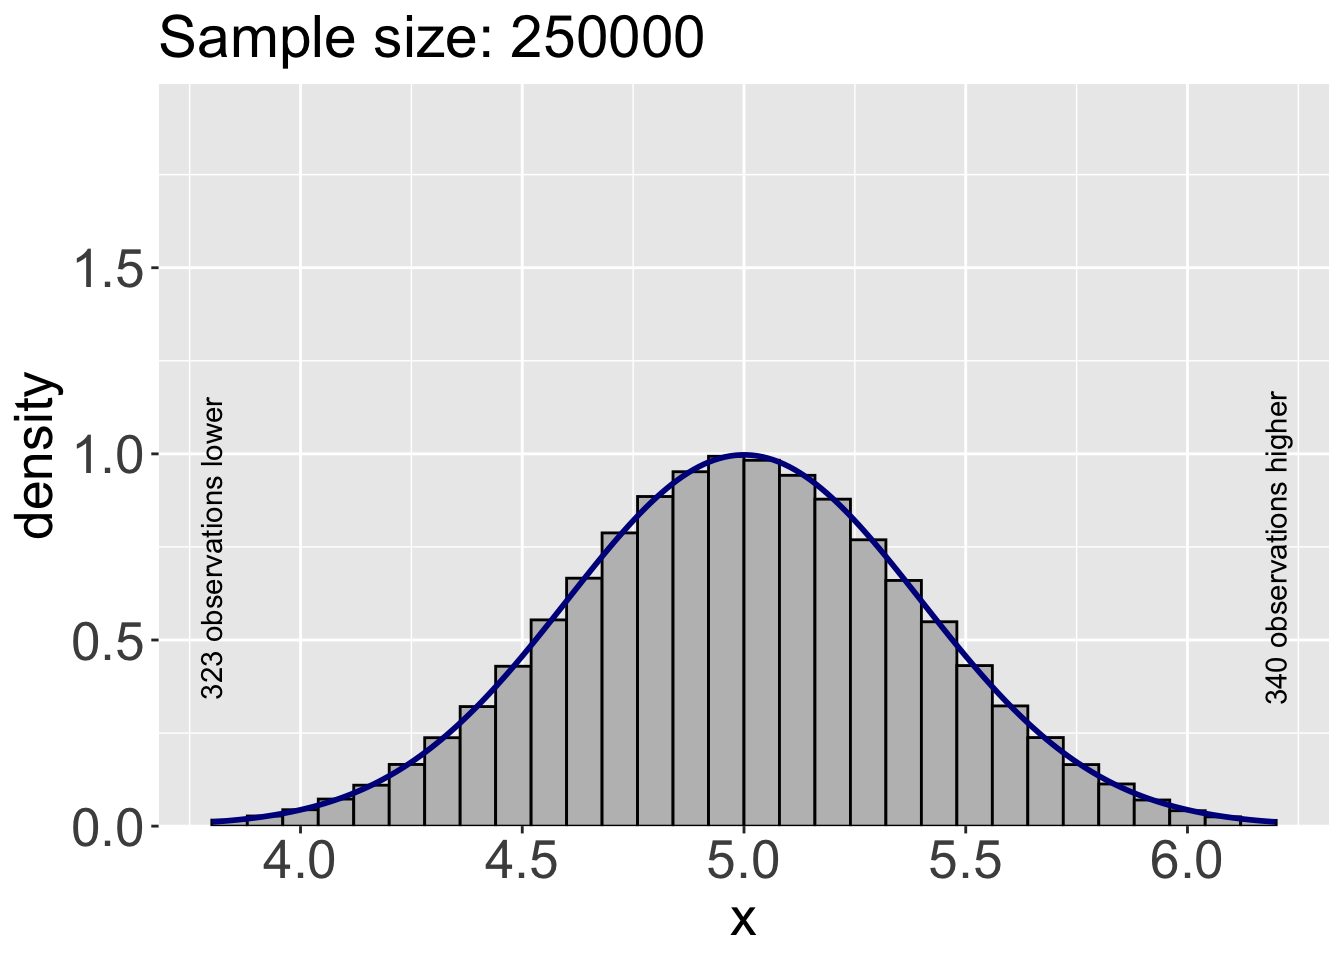
\includegraphics[width=0.24\linewidth]{book_files/figure-latex/rp_sample_population_plots-11} 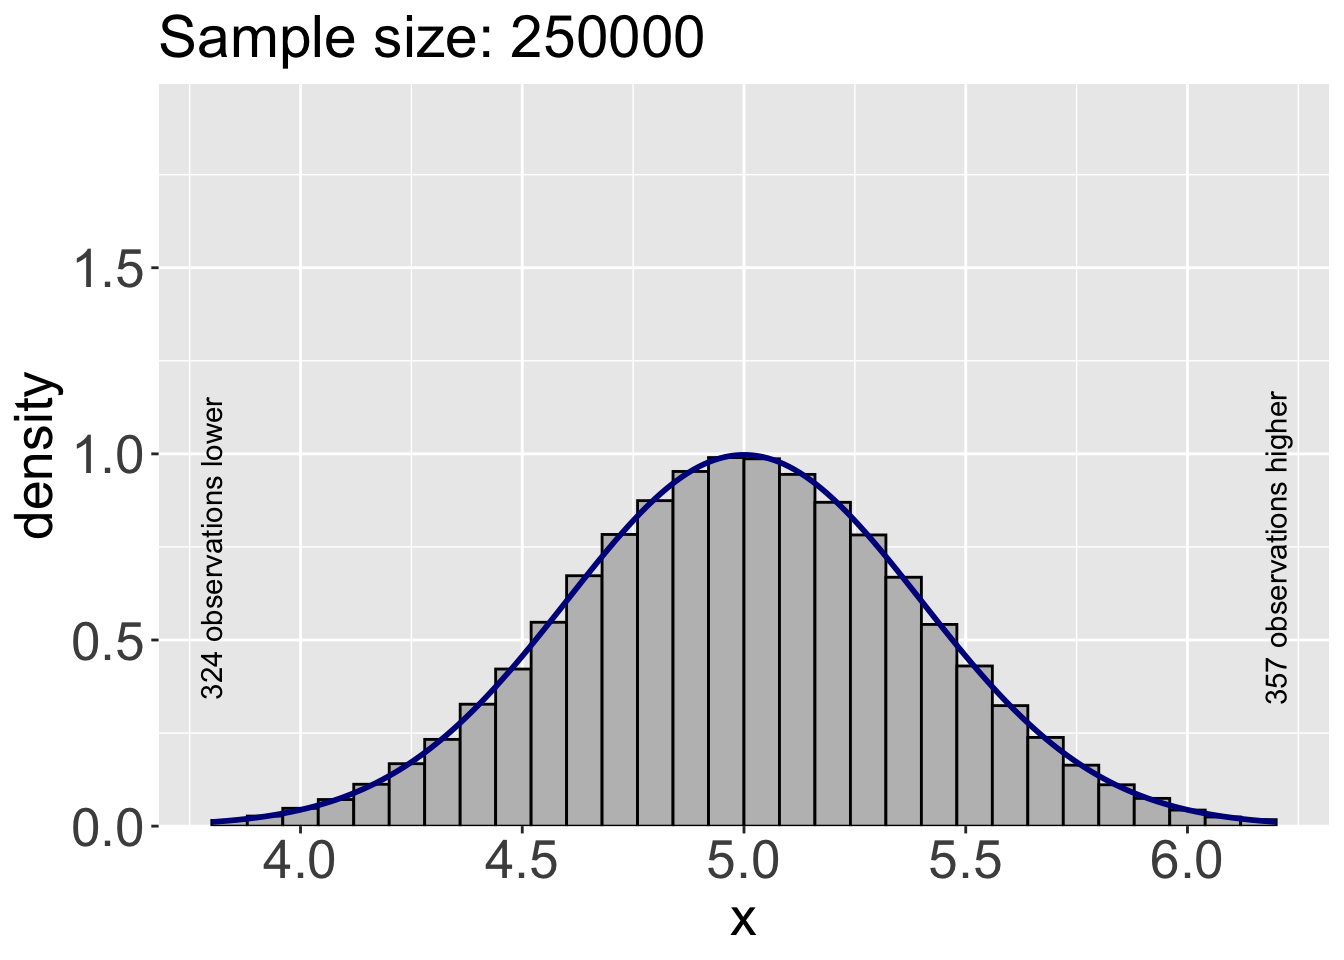
\includegraphics[width=0.24\linewidth]{book_files/figure-latex/rp_sample_population_plots-12}

The plots above shows histograms of multiple sets of sampled data. In each case the population is the same but the sample is different every time. It is the nature of variability that the particular data points we see, and so the details of the patterns which are displayed, change with every sample.

The first row of plots has sample size 25. Here there is a lot of variability in the shapes of the histograms. Sometimes there appear to be two clusters of data, or a rather skewed shape. We know that the underlying population is the same for all samples but the detailed shapes we see can be quite different. This tells us that we should be cautious in interpreting detailed patterns when the size of our sampled dataset is small.

The second row has sample size 2500 and here the variation in shape is much smaller. The third row of plots has sample size 250000. Now there is almost no variation in shape. The continuous curve shows the shape of the distribution from which the data were sampled and the histograms match this very closely every time. This illustrates the general principle that more data gives us more information, reducing the variability in the features of the population that the data express.

The continuous curve is what the histograms `converge' to as the sample size gets higher and higher and variability gets smaller and smaller (and the histogram bin width also get smaller and smaller). This is known as the \emph{density function} and it defines the population from which we are sampling. For any interval on the axis, the area under the density function gives the probability of an observation falling in this range so, in that sense, the density function describes how the probability of observing different values changes across the axis.

This particular population has a \emph{normal distribution}. This has a characteristic symmetric shape which falls away smoothly as we move to values further from the centre of the distribution. Just as the mean of a sample can be characterised as the `centre of gravity' of the dataset, so the mean of the distribution can be defined as the `centre of gravity' of the distribution. One consequence of the symmetry of the normal distribution is that the mean sits at its point of symmetry, where the density function reaches its highest value. In the present case the mean has the value 5. Similarly, the spread of the distribution around its mean value can be quantified by the standard deviation. Like the mean, this can be defined in terms of the density function but we can also simply regard it as the value to which the sample standard deviation converges as the sample size gets higher and higher. In the present case the population standard deviation is 0.4.

\begin{center}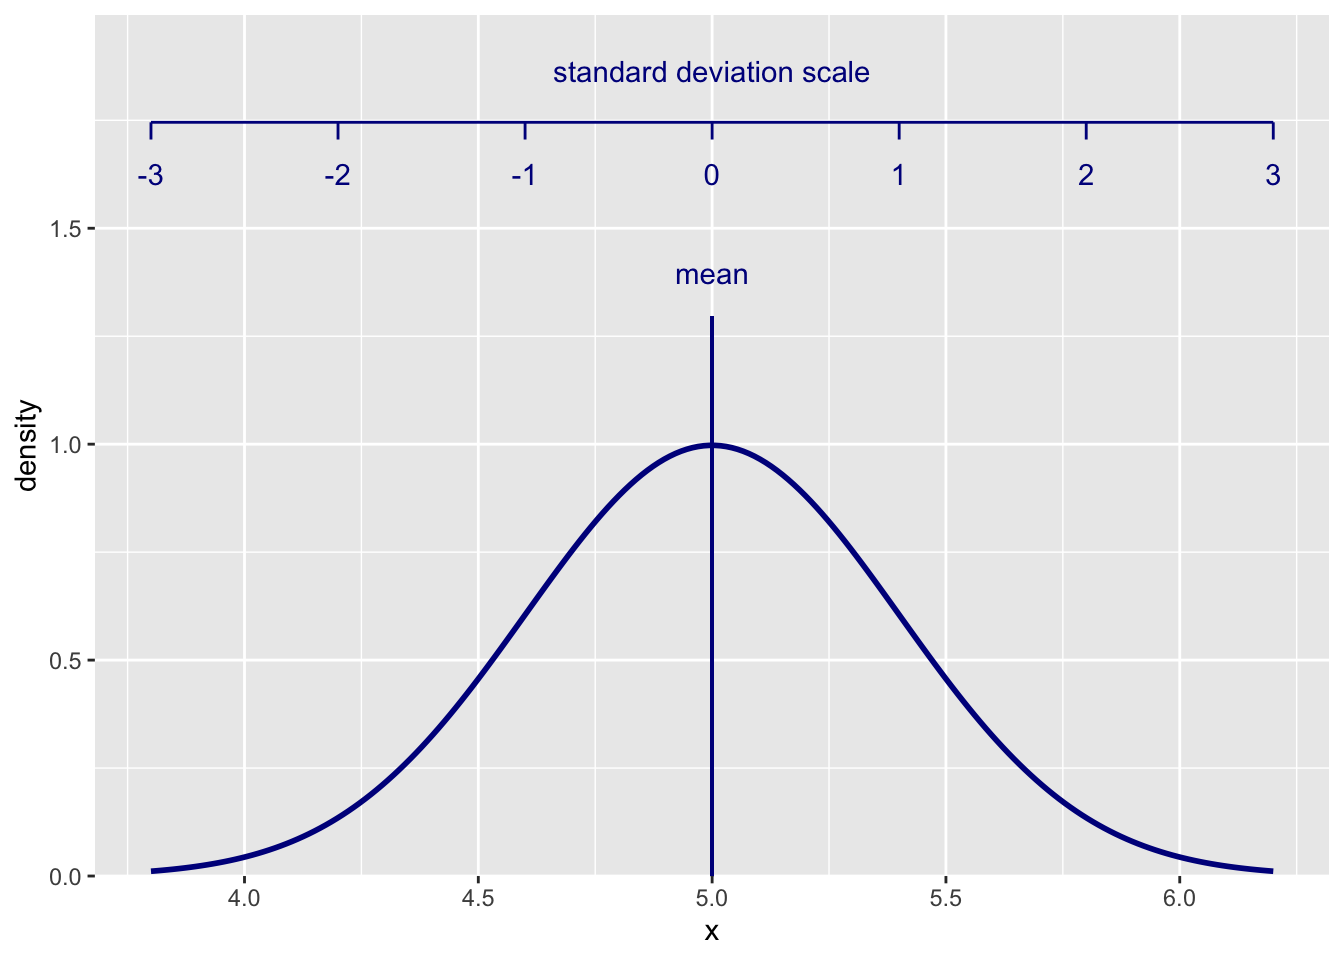
\includegraphics[width=0.49\linewidth]{book_files/figure-latex/rp_mean_se-1} \end{center}

The plot above shows the normal distribution, with the mean highlighted and with a superimposed scale which measures distance along the axis in units of standard deviation, so `1' lies at a distance of 0.4 from the mean, `2' at 0.8 and so on. This shows that most of the distribution lies within 2 standard deviations of the mean. This happens with samples too so that, most of the time, the observations in a sample lie within 2 standard deviations of the mean. The plots below illustrate this.

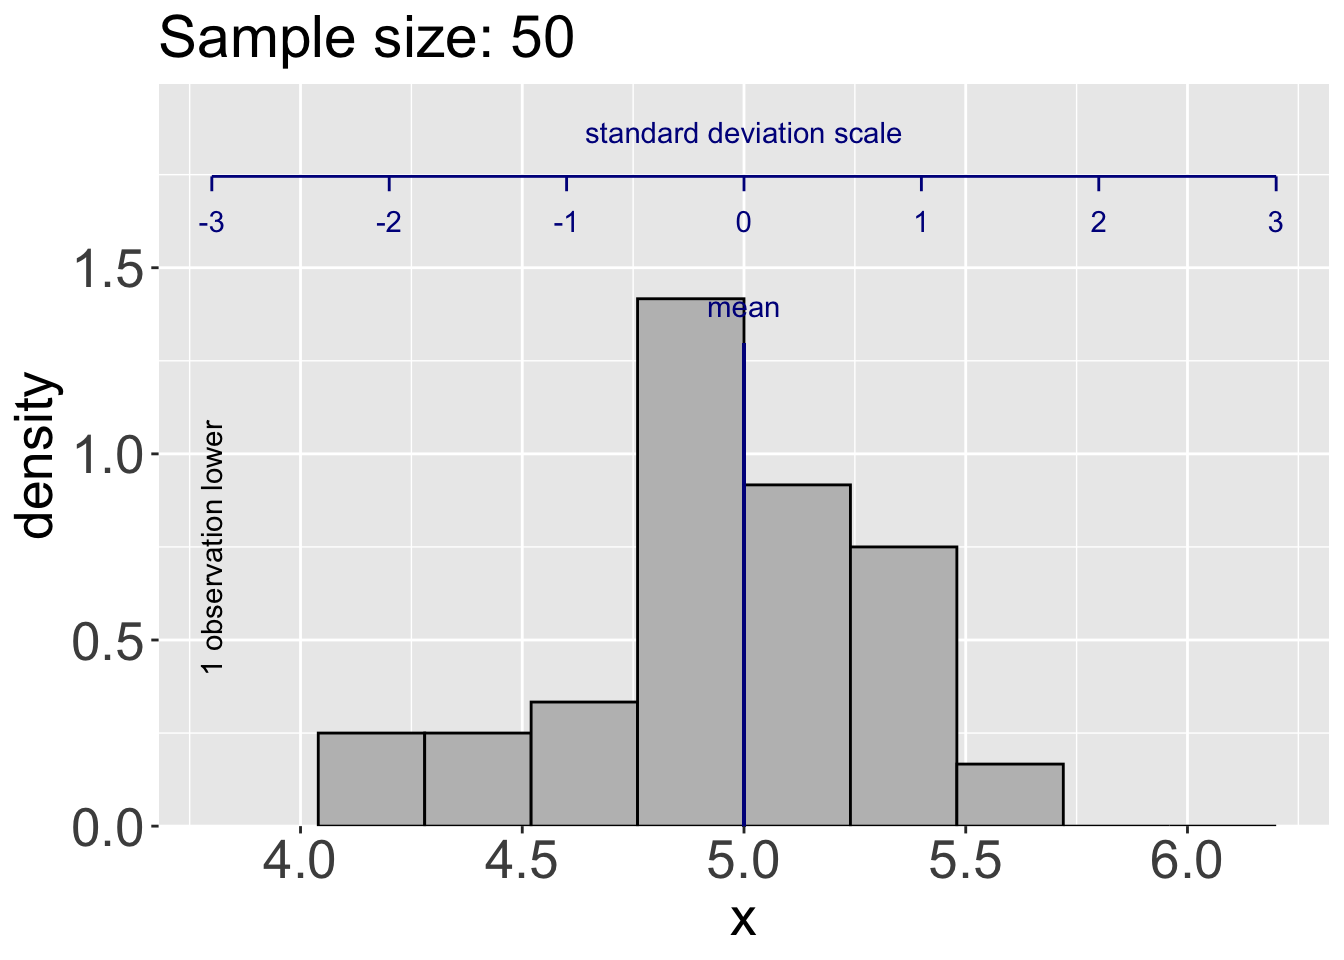
\includegraphics[width=0.24\linewidth]{book_files/figure-latex/rp_sample_se_plots-1} 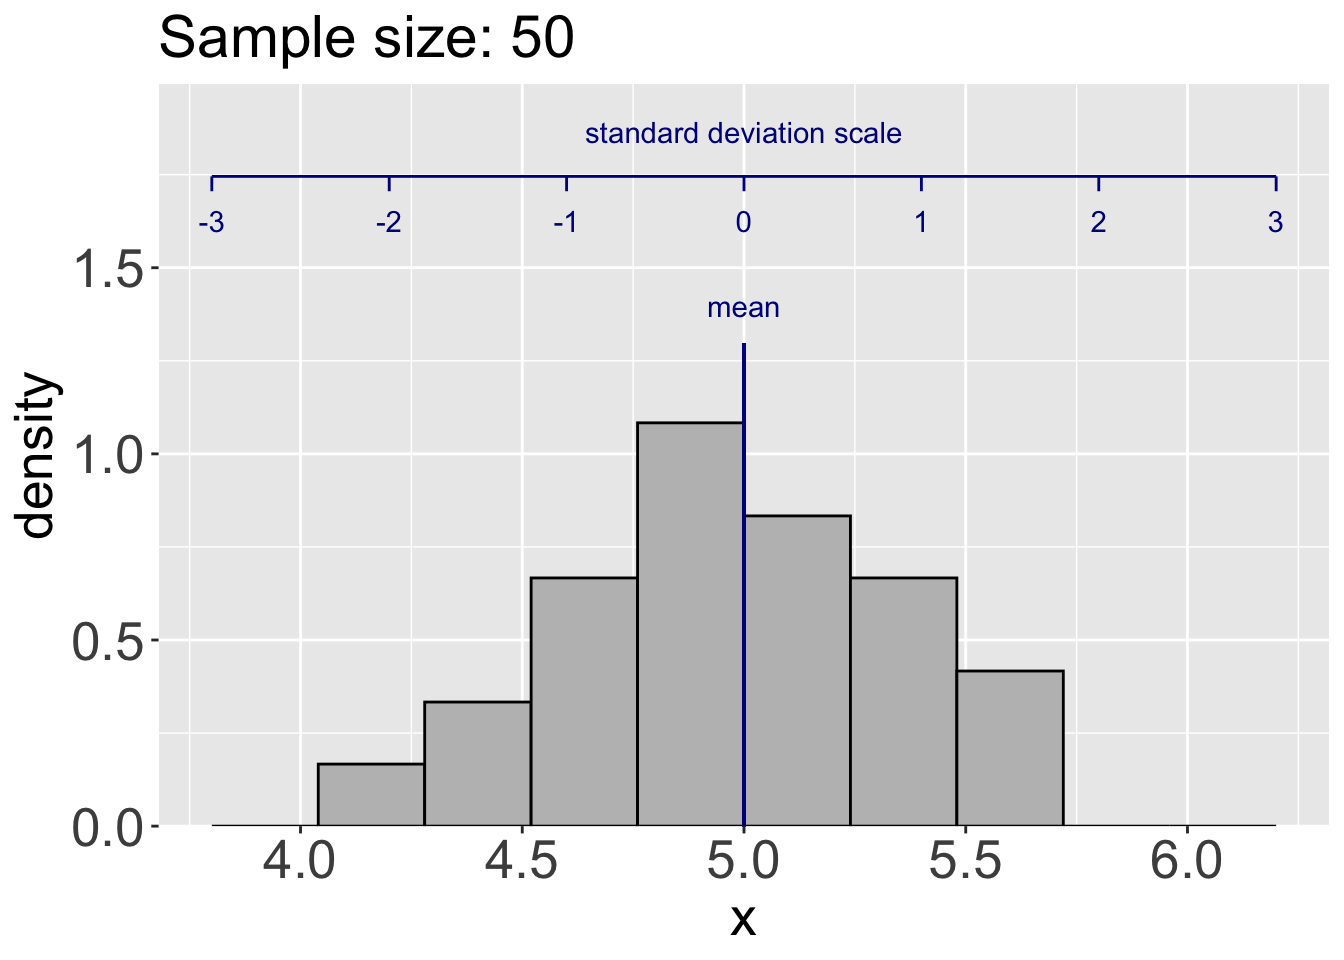
\includegraphics[width=0.24\linewidth]{book_files/figure-latex/rp_sample_se_plots-2} 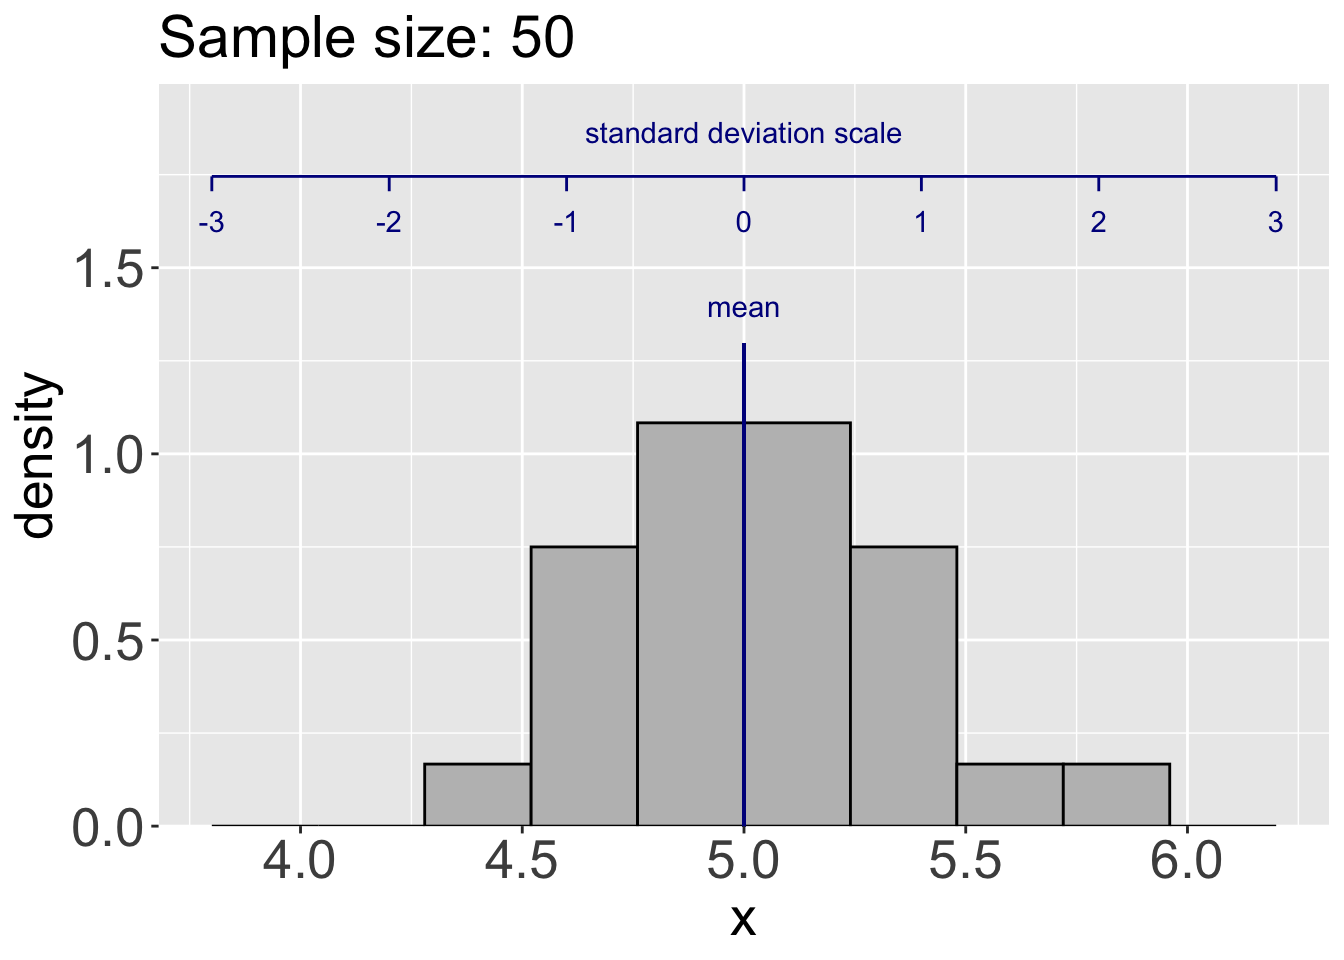
\includegraphics[width=0.24\linewidth]{book_files/figure-latex/rp_sample_se_plots-3} 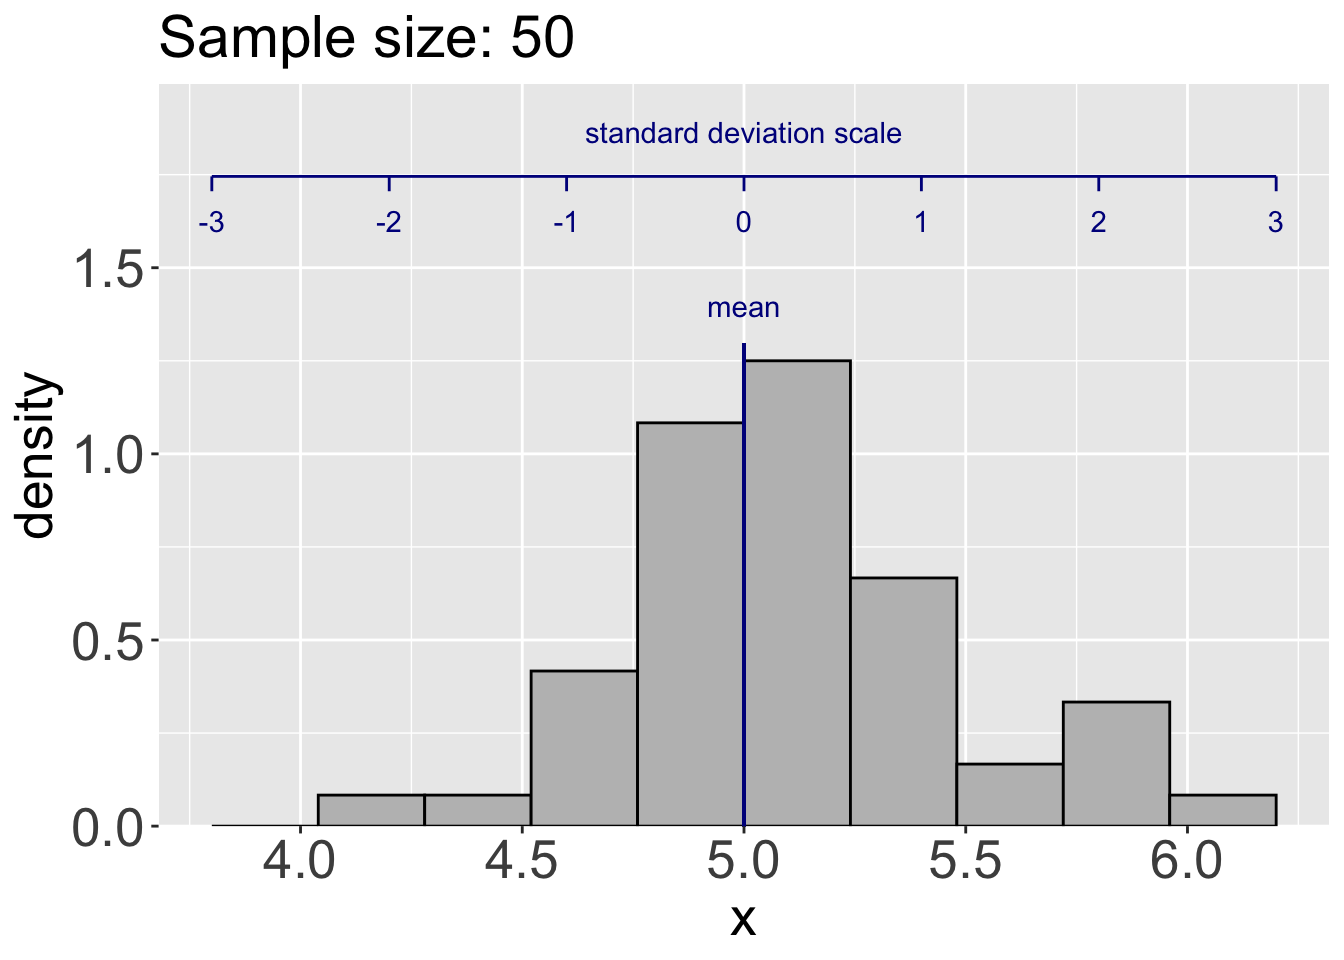
\includegraphics[width=0.24\linewidth]{book_files/figure-latex/rp_sample_se_plots-4}

This makes sense, as the standard deviation quantifies how far away observations are from the mean, on average. So, informally, one standard deviation away from the mean, on either side, takes us `halfway' into the spread of the data. From that perspective, it then seems reasonable that two standard deviations away from the mean should cover most of the observations in our sample. This works rather neatly for the normal distribution but in fact the general principle holds for many distributions, even ones which are not symmetric, although the guideline will become less effective as the size of skewness increases. An exercise in Section \ref{quantifying-uncertainty-exercises} below will invite you to explore this.

The normal distribution is a very important one for modelling measurements on a continuous scale but there are many other possible distributions. We will meet some of these in due course, as we encounter datasets with features which need other distributional shapes to describe them.

\section{Quantifying uncertainty: standard error}\label{quantifying-uncertainty-standard-error}

The `thought experiment' of the previous section explored the relationship between a sample and a population but this was necessarily set up rather artificially, as we defined (through the settings in \texttt{rp.sample}) the population from which the samples were being drawn. In practice, of course, a sample is all we have and we seek to use this to learn about the population - perhaps simply its mean, or perhaps other features of interest. This is why the title of the current chapter is `Inference', as we seek to infer features of the unknown population from the (usually rather limited) data in our sample.

We will explore this by continuing our thought experiment, using the population mean as the focus, as this is often a parameter of major interest. How accurate is the sample mean as a guide to the population mean? The \texttt{rp.sample} function can again help us think this through. The plots below show, in the upper row, multiple samples, each of size 25. The second row of plots shows the mean of each sample, with the final plot in this row showing sample means accumulated over 50 different samples. The sample means are clustered round the true mean. There is variation in the sample means but the size of this is much smaller than the variation in the individual observations.

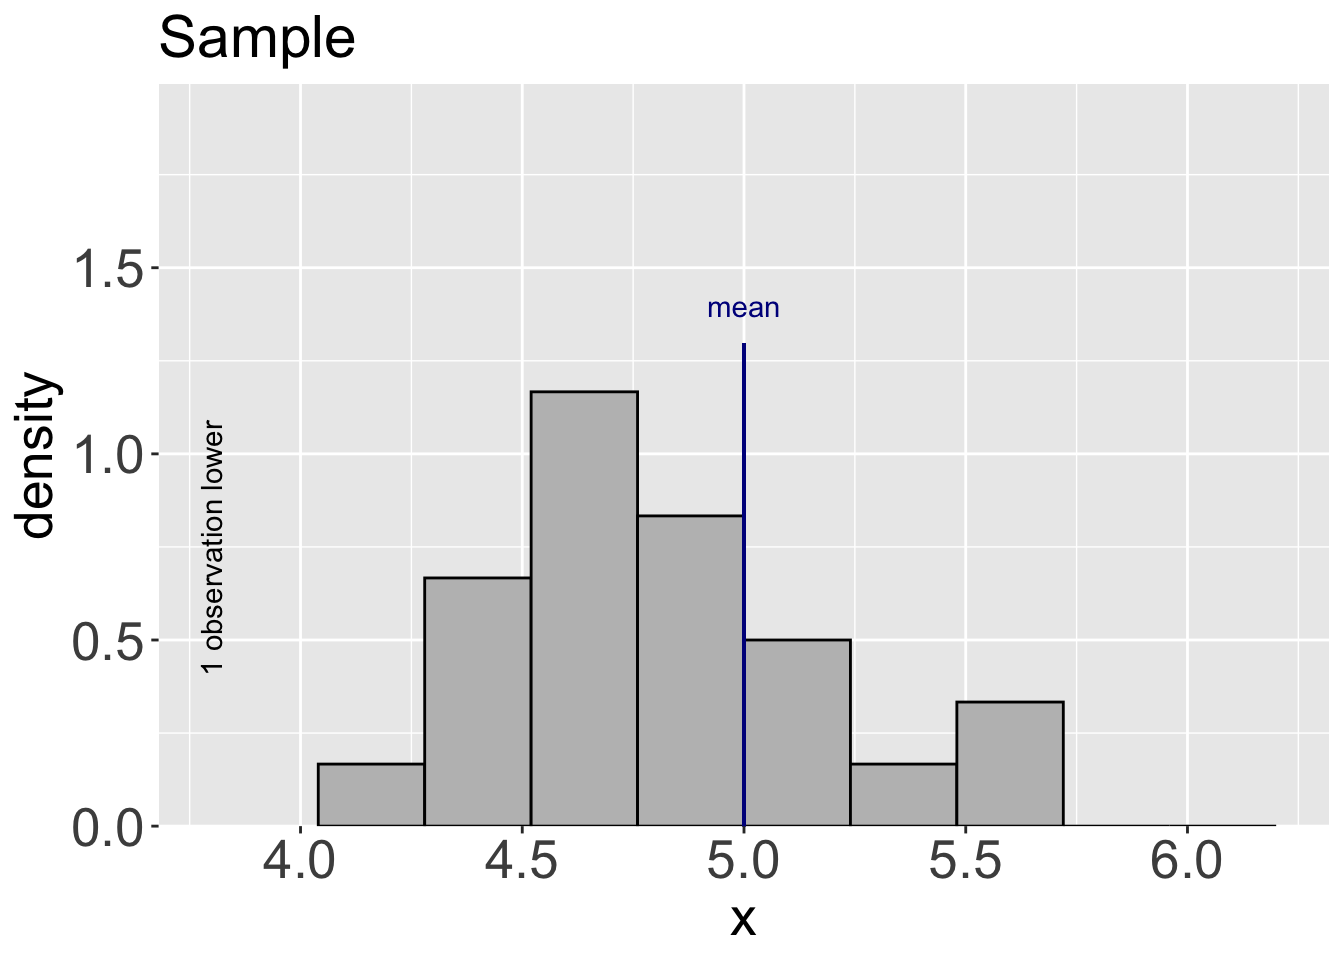
\includegraphics[width=0.24\linewidth]{book_files/figure-latex/sample_mean-1} 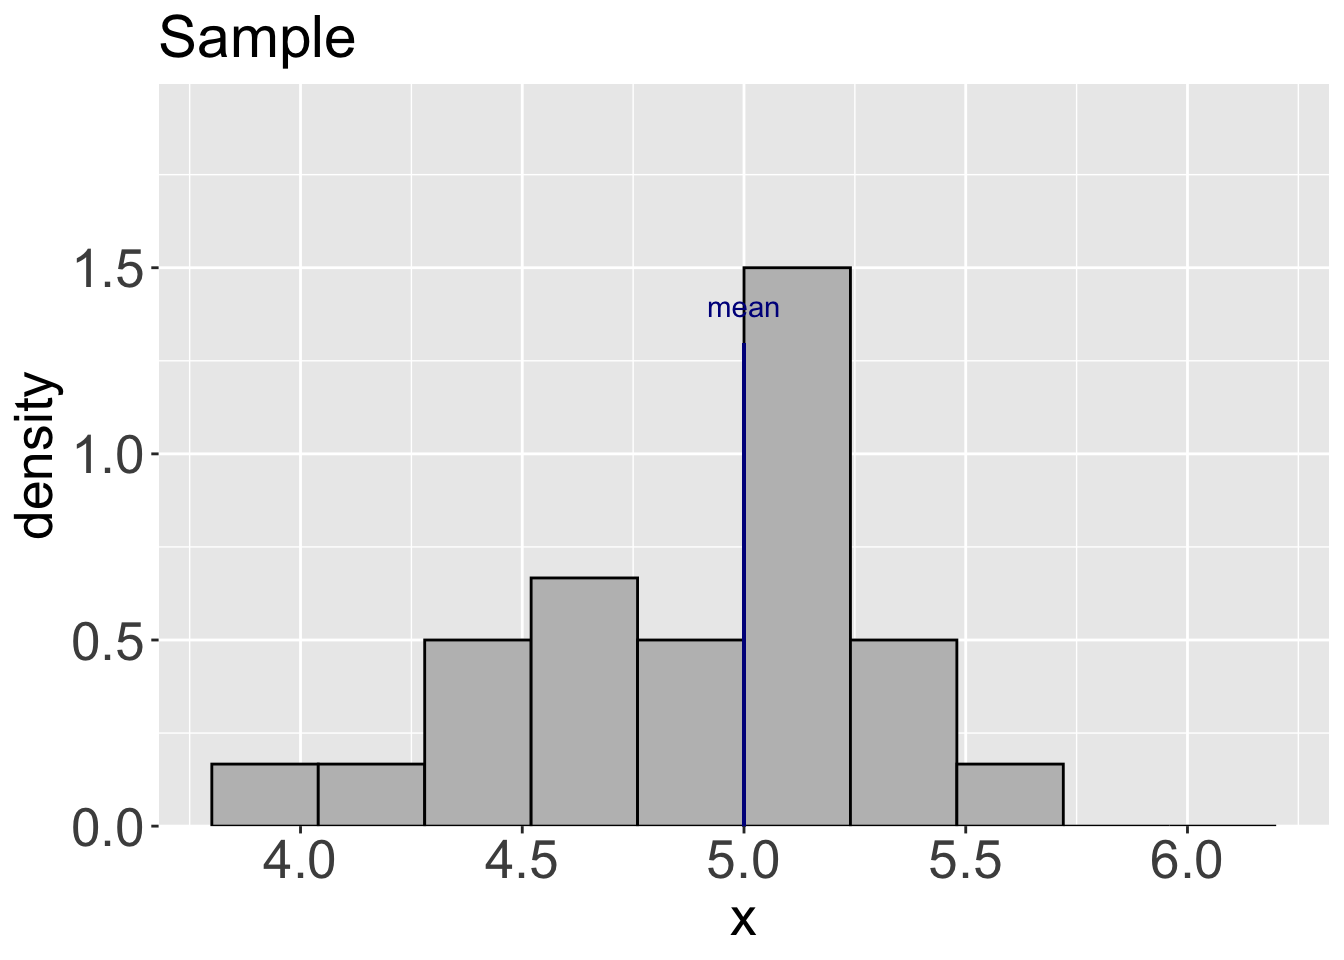
\includegraphics[width=0.24\linewidth]{book_files/figure-latex/sample_mean-2} 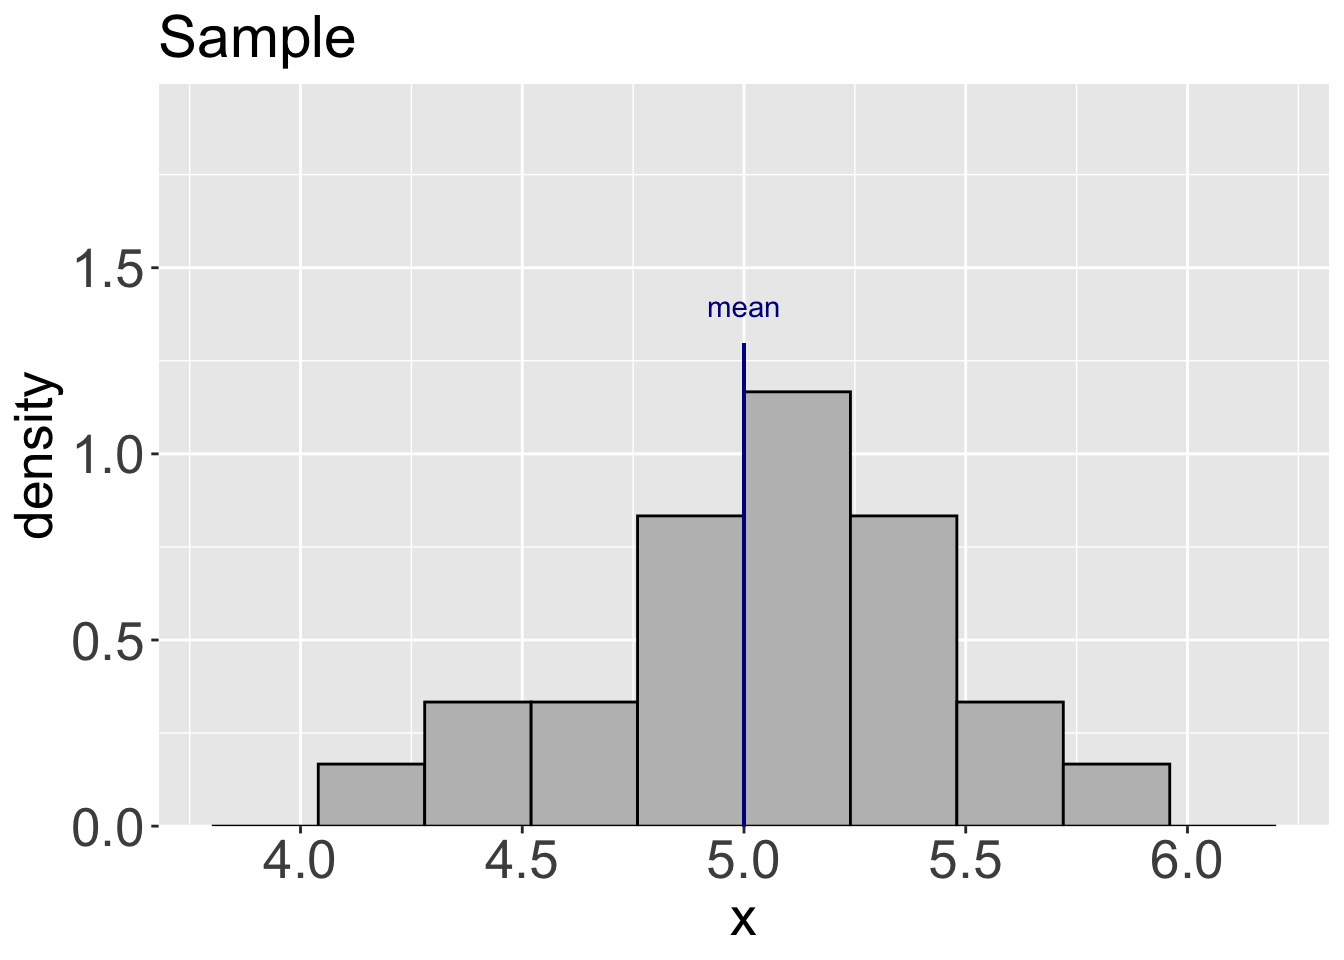
\includegraphics[width=0.24\linewidth]{book_files/figure-latex/sample_mean-3} 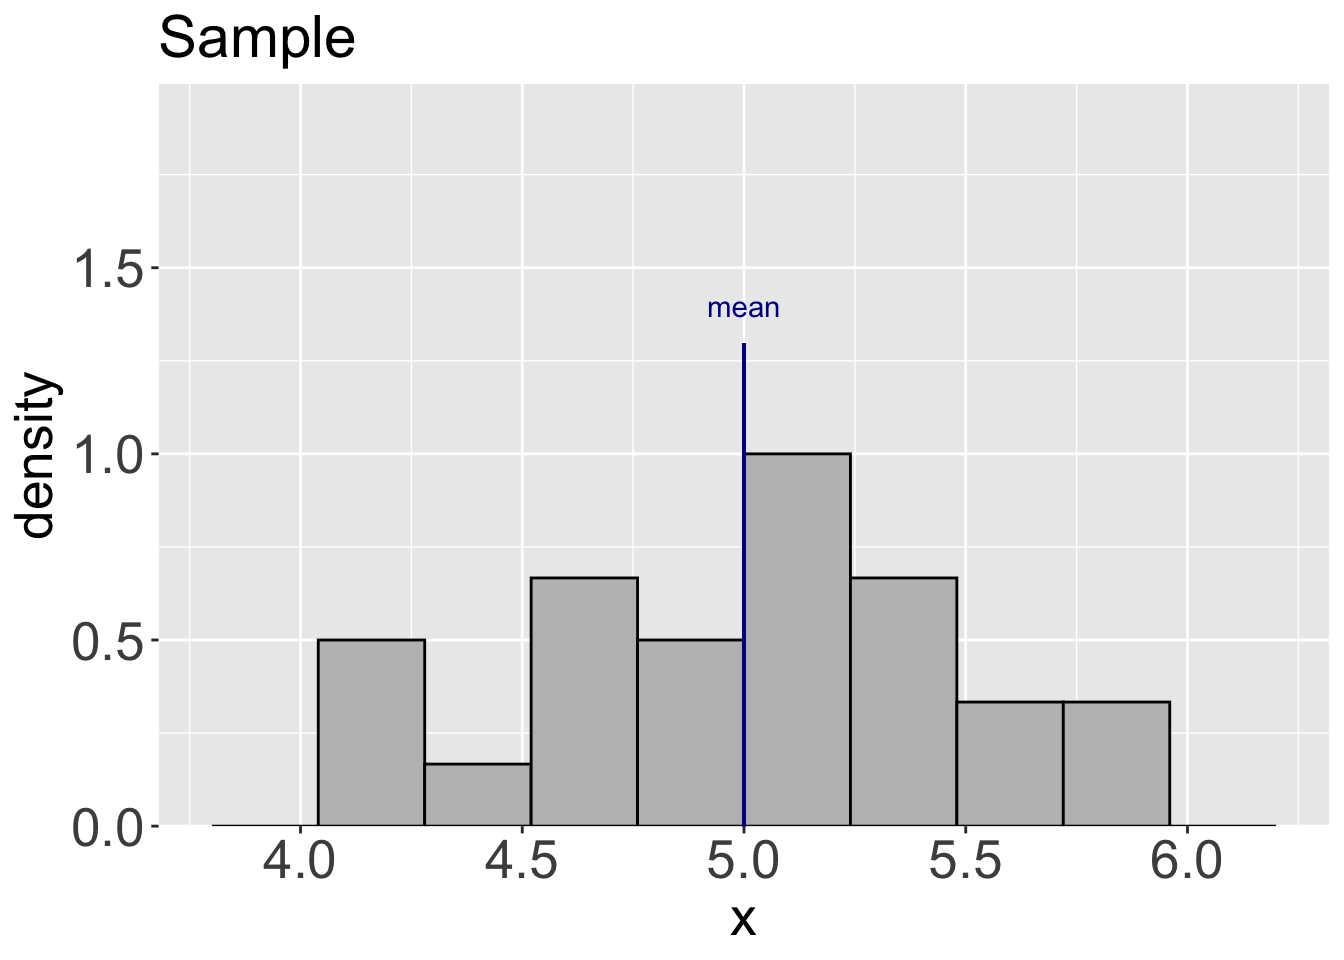
\includegraphics[width=0.24\linewidth]{book_files/figure-latex/sample_mean-4} 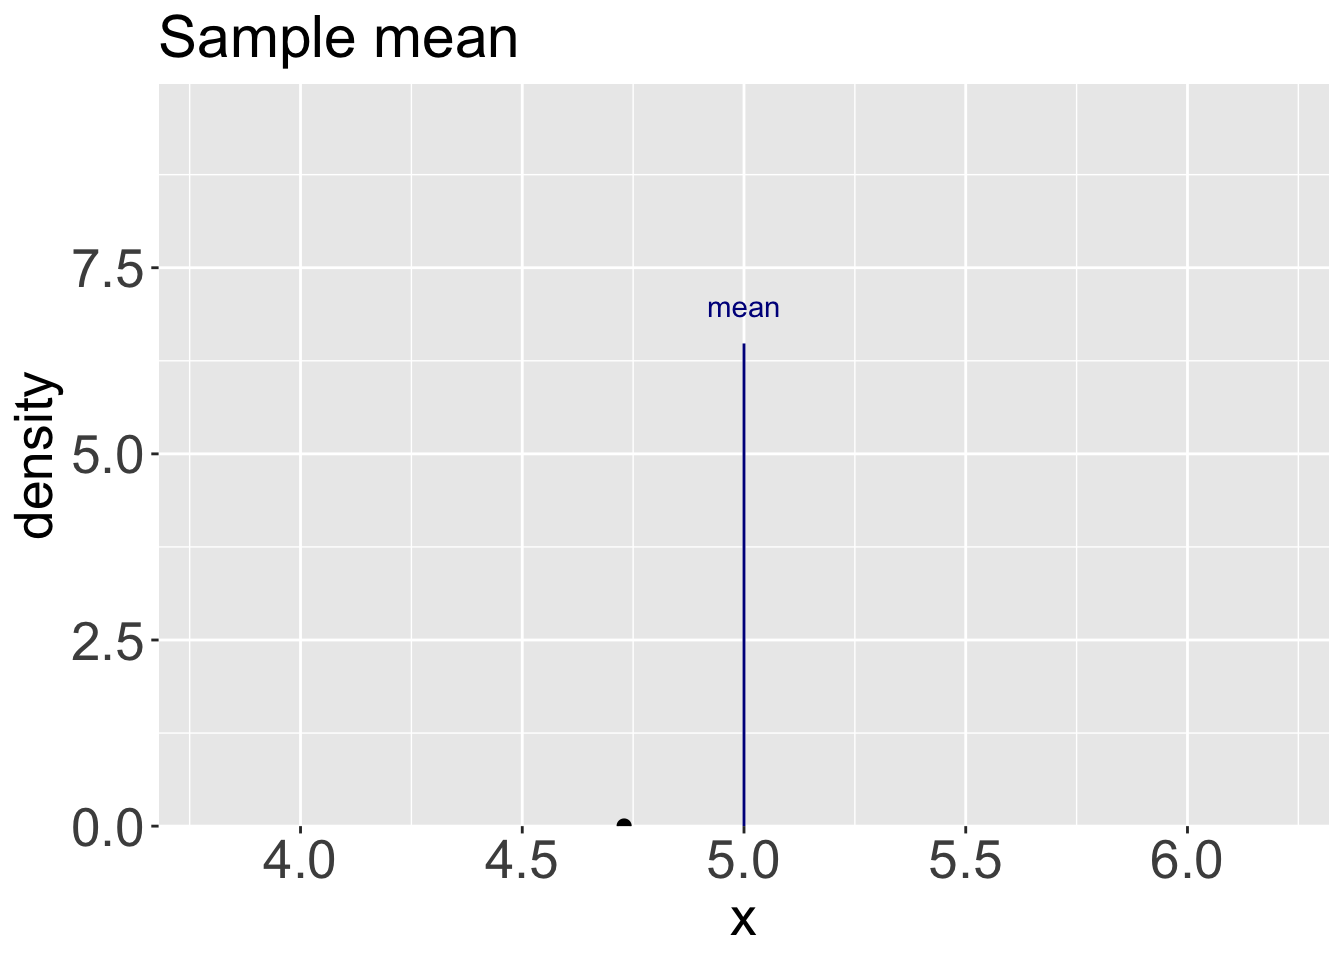
\includegraphics[width=0.24\linewidth]{book_files/figure-latex/sample_mean-5} 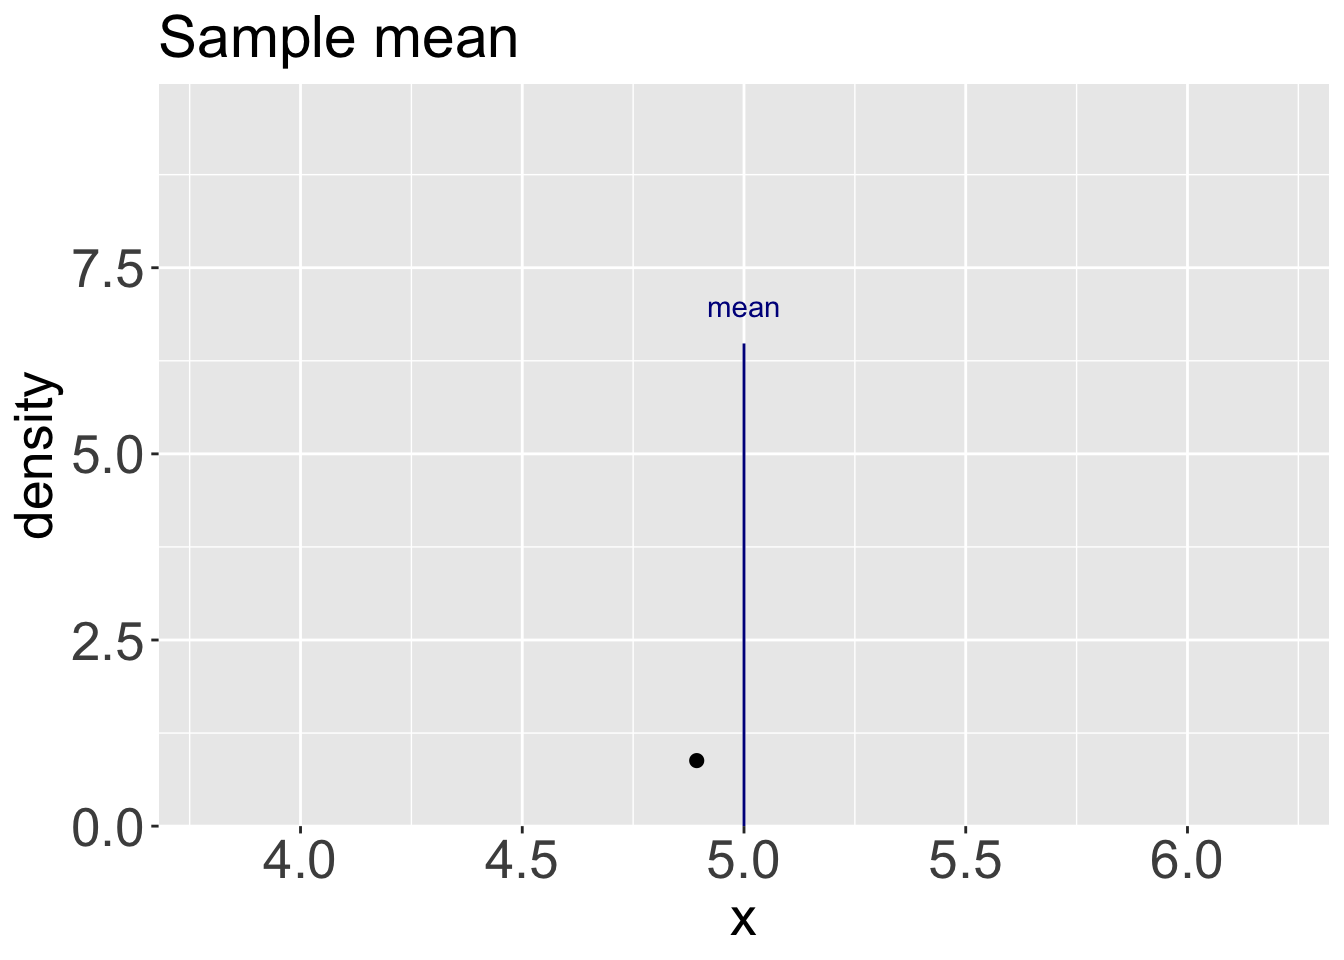
\includegraphics[width=0.24\linewidth]{book_files/figure-latex/sample_mean-6} 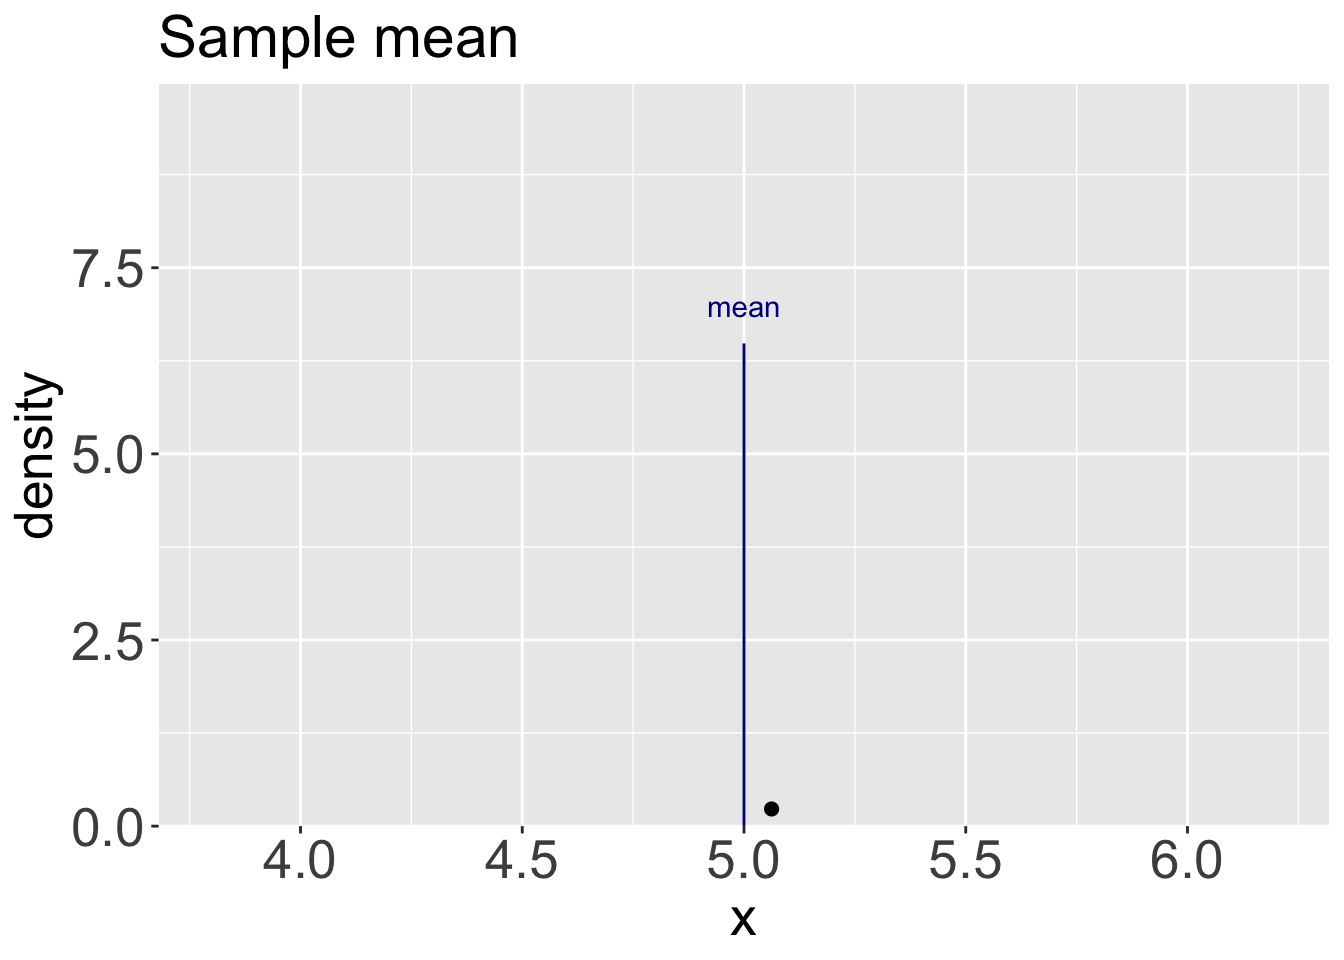
\includegraphics[width=0.24\linewidth]{book_files/figure-latex/sample_mean-7} 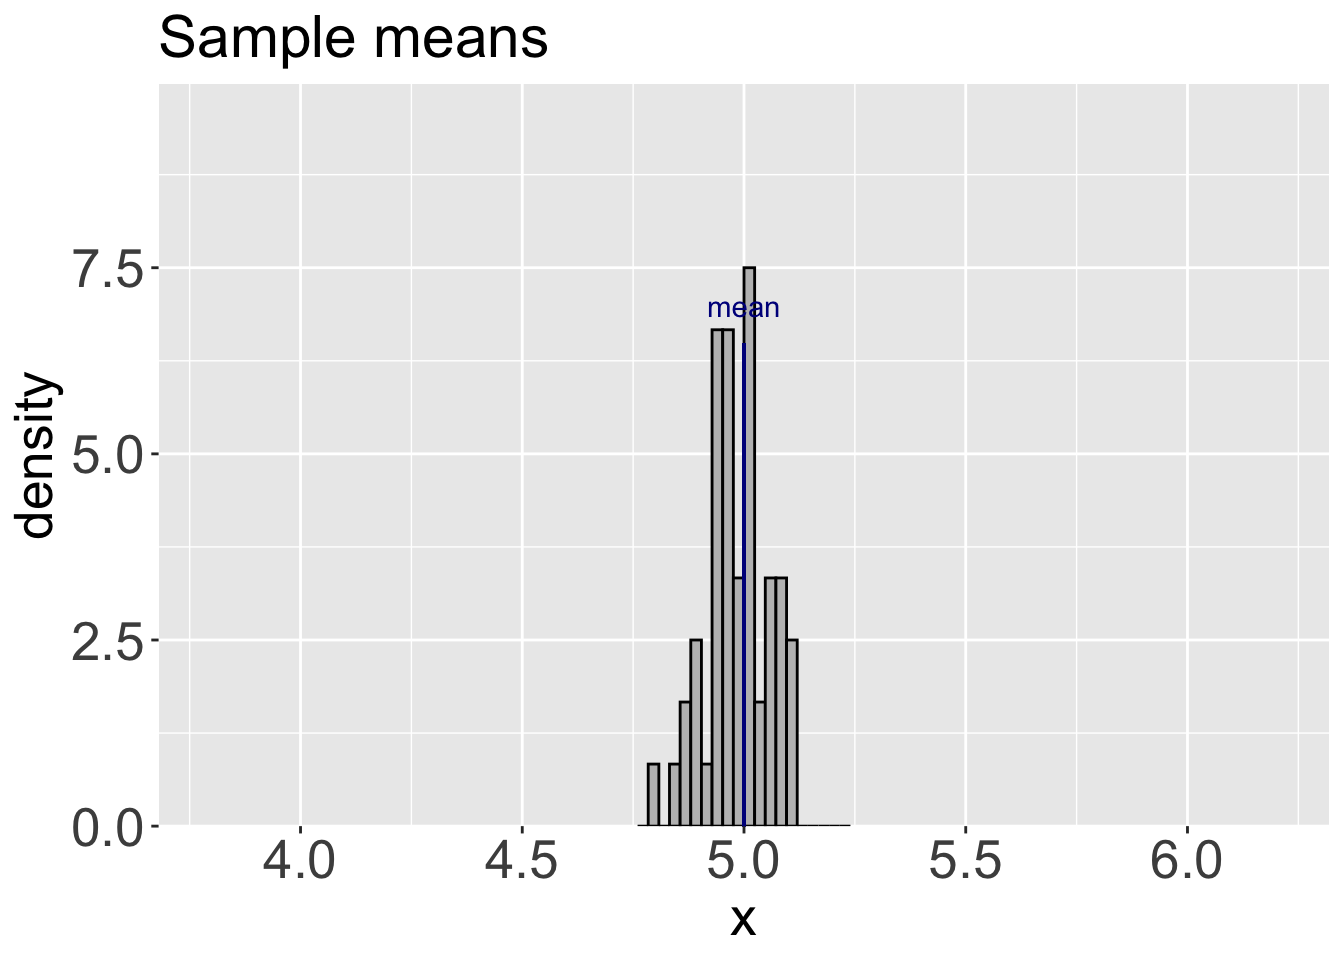
\includegraphics[width=0.24\linewidth]{book_files/figure-latex/sample_mean-8}

This is the point at which some theory can help us. This shows that the standard deviation of the sample mean, known as the \emph{standard error}, can be easily calculated as
\[
   \mbox{se}(\bar{x}) =  \sigma / \sqrt{n} .
\]
This gives us a measure of uncertainty, or inaccuracy, of the sample mean \(\bar x\) as an estimate of the true mean \(\mu\). In practice, we would estimate this as \(s / \sqrt{n}\).

\begin{center}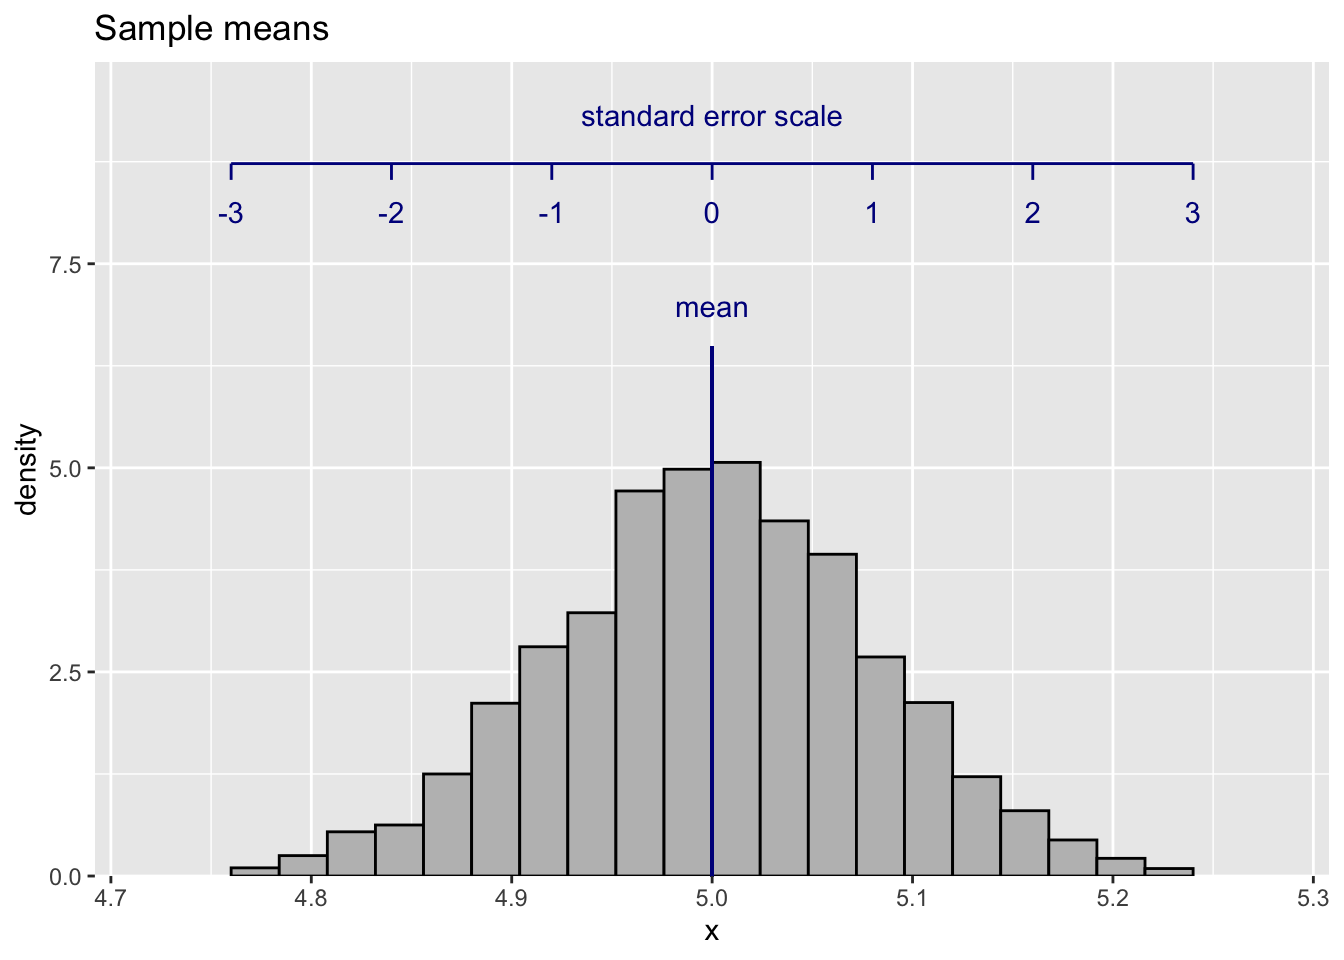
\includegraphics[width=0.7\linewidth]{book_files/figure-latex/sample_mean_se-1} \end{center}

This is a very important fact which we should pause to highlight in general terms of a true \emph{parameter}, here the mean \(\mu\), and an \emph{estimate} of it, here the sample mean \(\bar x\).

\begin{verbatim}
                              Most of the time,
   the true parameter and the estimate are within 2 standard errors of one another.
\end{verbatim}

The sample mean has a distribution. If we knew what this was then we could quantify the uncertainty of the mean of our sample.
Theoretical calculations tell us that the sample mean also has a normal distribution, that it's mean is the mean of the original distribution, and we can derive an expression for the standard deviation of this distribution. Formula.

Estimated standard error. t-statistic. t-distribution.

This very important principle will be the basis of the tools we now develop.

\section{Confidence intervals}\label{confidence-intervals}

This statement describes how the sample means \(\bar x\) varies around the true mean \(\mu\). In practice all we see from our observed sample of data is a single \(\bar x\) and its estimated standard error. However, we can turn the statement around and expect that the true value of \(\mu\) will lie somewhere within 2 standard errors of \(\bar x\). The interval
\[
      ( \bar{x} - 2 \mbox{se}(\bar x), \bar{x} + 2 \mbox{se}(\bar x) )
\]
is therefore a range of plausible values for the true mean \(\mu\). This is called a \emph{confidence interval} because we can attach some useful proporties of this kind of interval; these are discussed below. We can also carry out some more careful probability calculations which show that, while the multiplier 2 is a good approximation, a more precise value is the percentile of a \(t\)-distribution with \((n-1)\) \emph{degrees of freedom}.

The first person to propose this idea was W.S.Gossett, in a famous paper in 1908. He published under the pseudonym \emph{Student} because he was working for the \emph{Guiness} brewery at the time. He used data from a paper by Cushny \& Peebles (1905) which compared the effects of two different drugs on lengthening the hours of sleep in 10 different subjects. The experimental design involved each subject taking each of the two drugs, so this is \emph{paired} data. A helpful first step is to plot the paired values against one another, with the line \texttt{y\ =\ x} providing a reference. If there is no systematic difference between the effects of the drugs then the observations should cluster around this line.

\begin{Shaded}
\begin{Highlighting}[]
\NormalTok{sleep\_wide }\OtherTok{\textless{}{-}} \FunctionTok{pivot\_wider}\NormalTok{(sleep, }\AttributeTok{values\_from =}\NormalTok{ extra, }\AttributeTok{names\_from =}\NormalTok{ group,}
                          \AttributeTok{names\_prefix =} \StringTok{\textquotesingle{}drug\_\textquotesingle{}}\NormalTok{)}
\FunctionTok{ggplot}\NormalTok{(sleep\_wide, }\FunctionTok{aes}\NormalTok{(drug\_1, drug\_2)) }\SpecialCharTok{+} \FunctionTok{geom\_point}\NormalTok{() }\SpecialCharTok{+}
   \FunctionTok{geom\_abline}\NormalTok{(}\AttributeTok{slope =} \DecValTok{1}\NormalTok{, }\AttributeTok{col =} \StringTok{\textquotesingle{}blue\textquotesingle{}}\NormalTok{, }\AttributeTok{linetype =} \DecValTok{2}\NormalTok{)}
\end{Highlighting}
\end{Shaded}

\begin{center}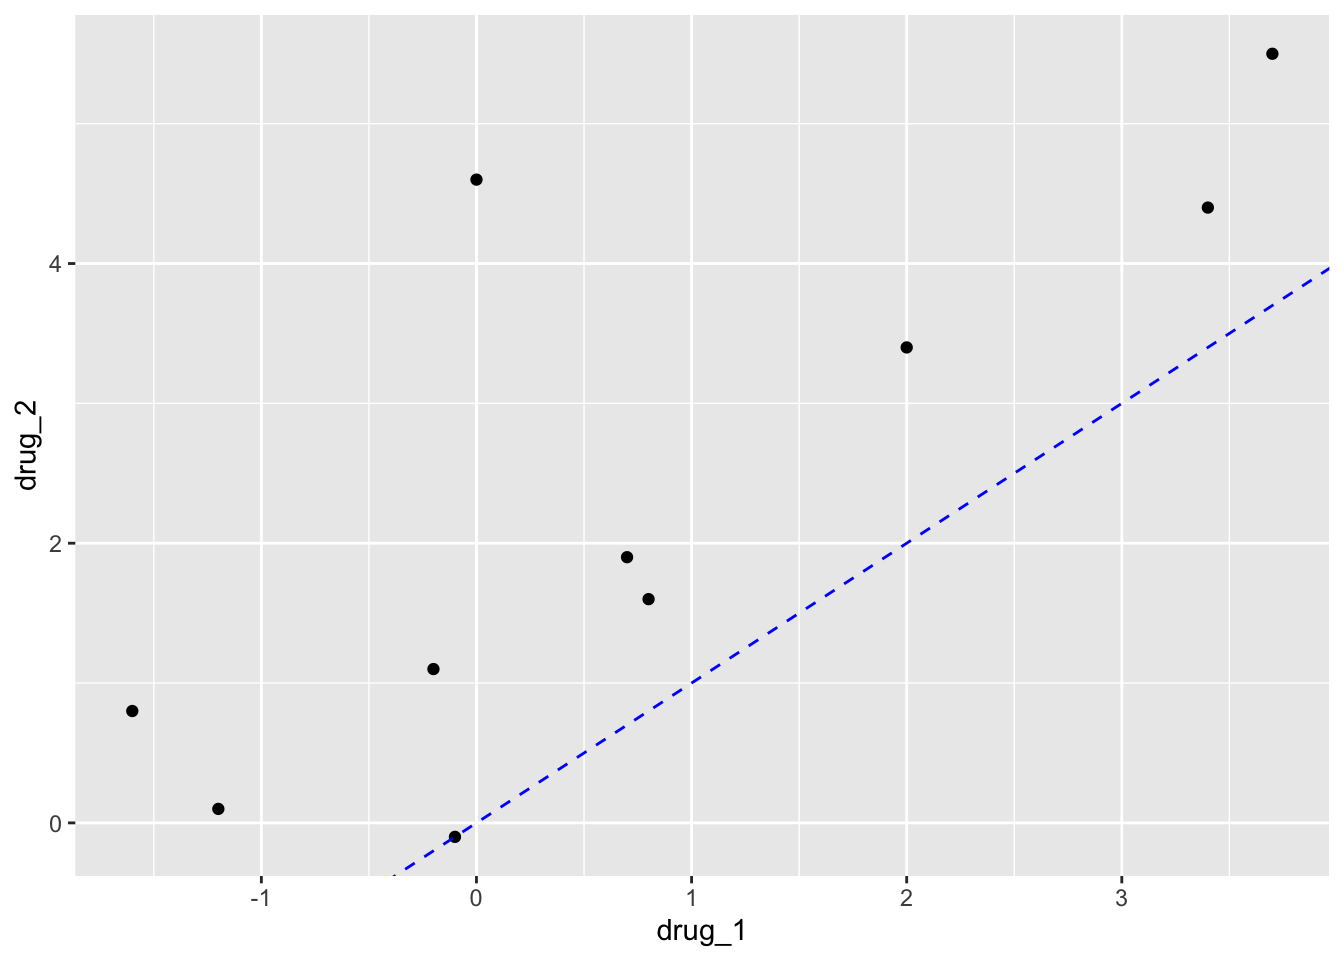
\includegraphics[width=0.7\linewidth]{book_files/figure-latex/sleep-1} \end{center}

The extra times for drug 2 are higher than those for drug 1, apart from one patient where the times were identical. In one patient the difference between the two drugs is particularly large but otherwise the differences are broadly similar. In particular, there is no obvious change in the size of the difference as the size of the response to drug 1 changes. This allows us to focus on the differences of the responses from the two drugs as the key information to analyse.

\begin{Shaded}
\begin{Highlighting}[]
\NormalTok{sleep\_diff }\OtherTok{\textless{}{-}} \FunctionTok{with}\NormalTok{(sleep\_wide, drug\_2 }\SpecialCharTok{{-}}\NormalTok{ drug\_1)}
\FunctionTok{rp.t\_test}\NormalTok{(sleep\_diff)}
\FunctionTok{rp.t\_test}\NormalTok{(sleep\_diff, }\AttributeTok{mu =} \DecValTok{0}\NormalTok{)}
\end{Highlighting}
\end{Shaded}

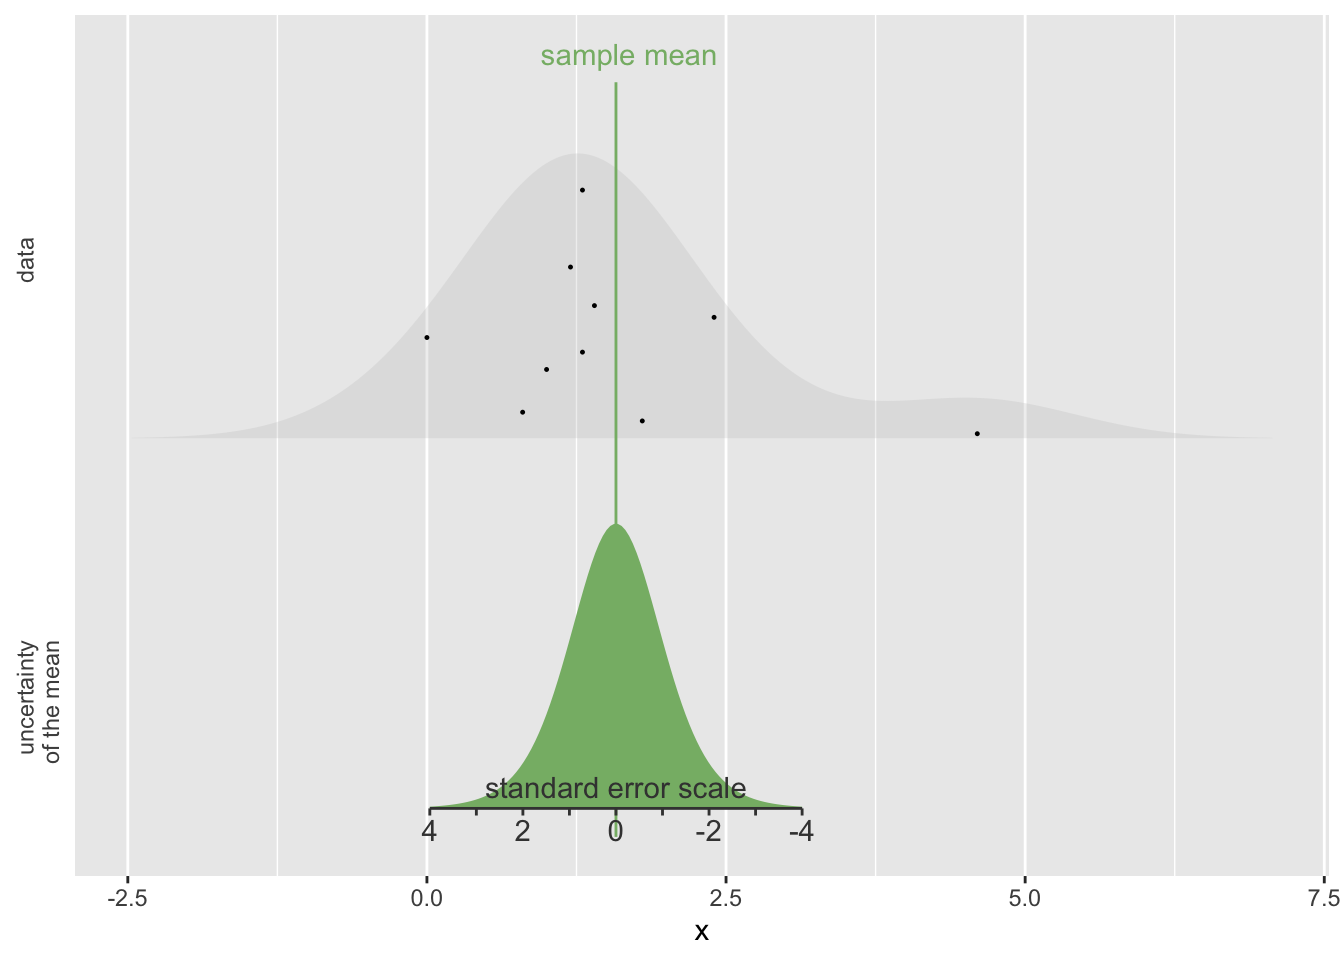
\includegraphics[width=0.49\linewidth]{book_files/figure-latex/sleep_uncertainty-1} 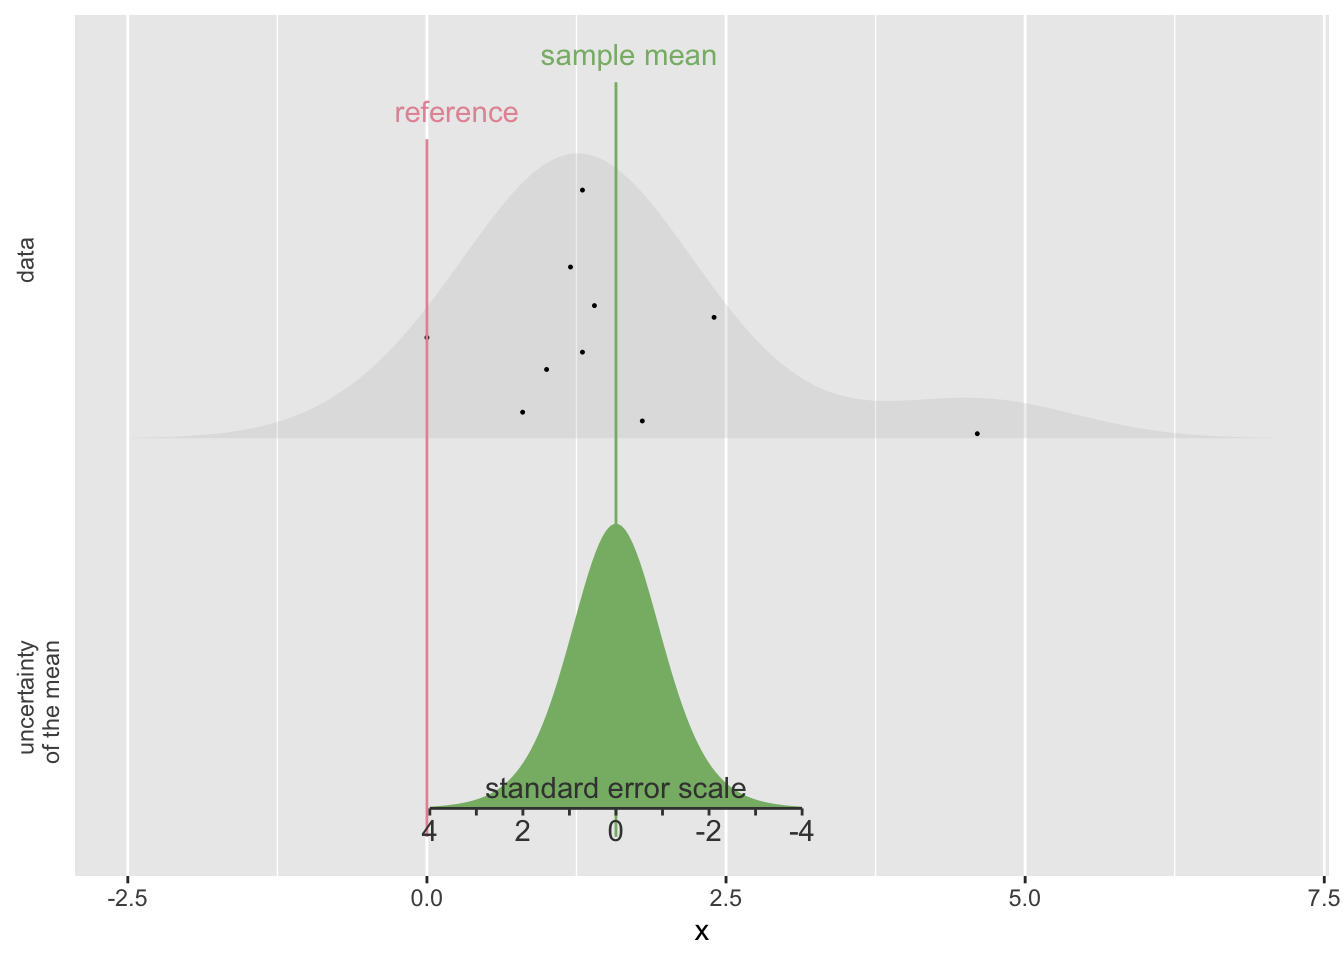
\includegraphics[width=0.49\linewidth]{book_files/figure-latex/sleep_uncertainty-2}

Comment that the areas of the data density and uncertainy distribution are not comparable. It is only relative sizes within in each distribution which matter.

Discuss the construction of a confidence interval.

Two sample example.

Relegate rp.ci to an exercise?

The meaning of a confidence interval sometimes causes a bit of confusion. The interpretation as a range of plausible values for the quantity we are estimating is a helpful but informal one. To explore the formal properties a little further we can experiment with the \texttt{rp.ci} function in the \texttt{rpanel} package for \texttt{R}. An example is shown below. Here we randomly sample 30 observations from a distribution with mean 0 and standard deviation 1 and compute a confidence interval for the mean. However, we do this 100 times. Each interval will be different because it is based on a different random sample of data. The \emph{confidence} of the intervals is conventionally set at 95\% and this is done by choosing percentiles in the confidence interval formula which capture 95\% of the \(t\)-distribution. Then, on average over repeated random samples, the computed confidence intervals will capture the true value 95\% of the time. Any particular set of 100 intervals will not have exactly 95 which capture the true value but if we keep repeating this and accumulate the tally, the proportion of intervals which capture the true value will settle down to 95\%.

\begin{center}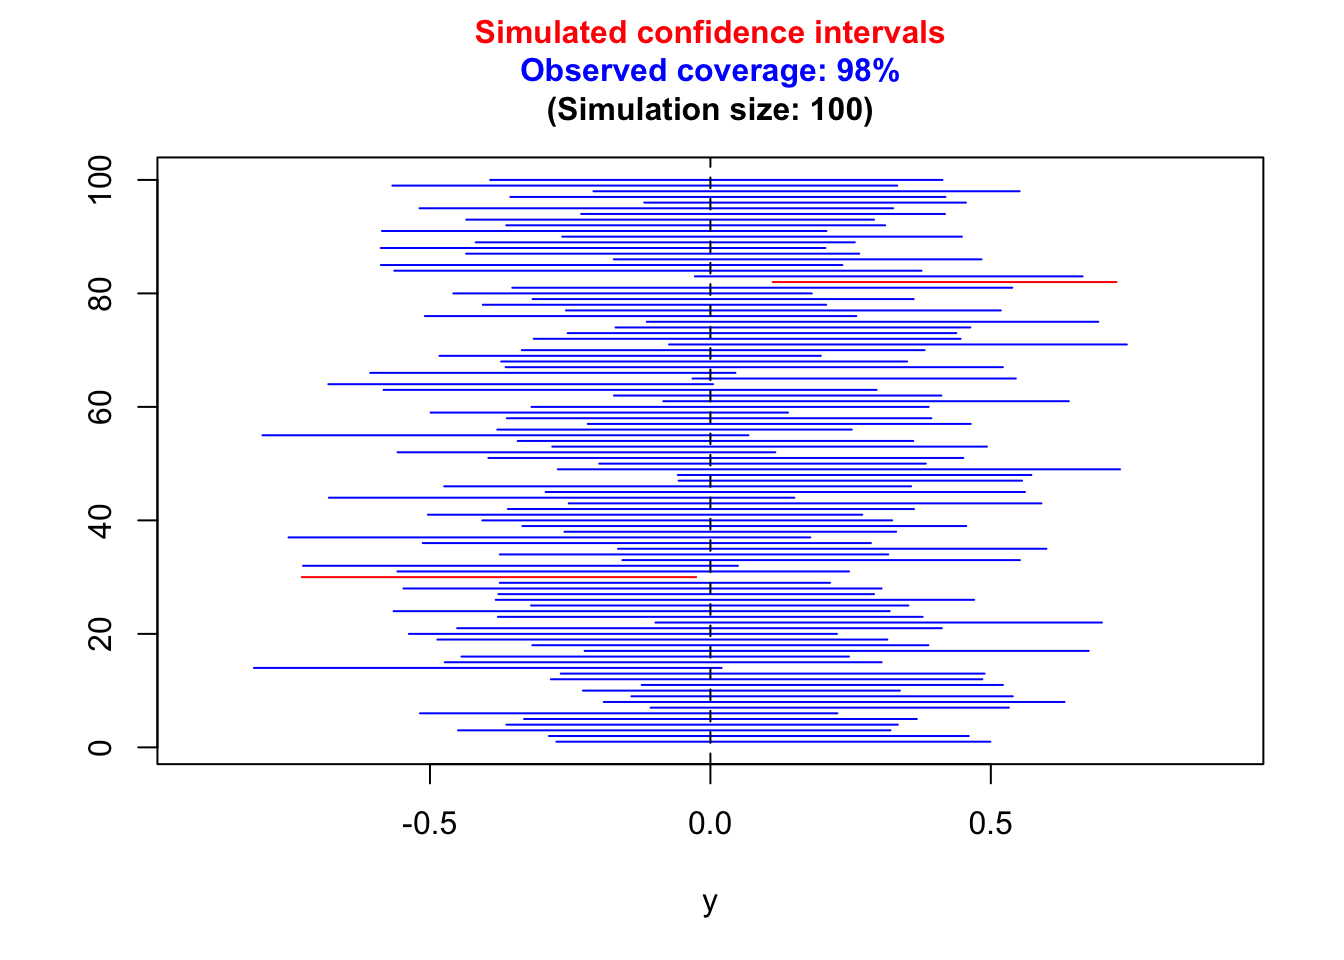
\includegraphics[width=0.5\linewidth]{book_files/figure-latex/coverage-1} \end{center}

\section{Hypothesis tests}\label{hypothesis-tests}

This way of thinking is based on weighing the available evidence to distinguish between two hypotheses. For example, if we have a sample of data there may be interest in examining whether it is plausible that the mean takes a particular value, say \(\mu_0\). If the measurements are differences in blood pressure between two time points for a set of patients, we may be interested in whether the mean of the measurements is 0, indicating no change in the mean, or not. The hypotheses are:

Null hypothesis: \(\mu = \mu_0\)\\
Alternative hypothesis: \(\mu \neq \mu_0\)

To distinguish between these hypothesis we can use again the helpful principle we identified in the discussion of samples and populations above.

\begin{verbatim}
                              Most of the time,
   the true parameter and the estimate are within 2 standard errors of one another.
\end{verbatim}

\begin{Shaded}
\begin{Highlighting}[]
\FunctionTok{rp.t\_test}\NormalTok{(sleep\_diff, }\AttributeTok{uncertainty =} \StringTok{\textquotesingle{}reference\textquotesingle{}}\NormalTok{)}
\end{Highlighting}
\end{Shaded}

\begin{center}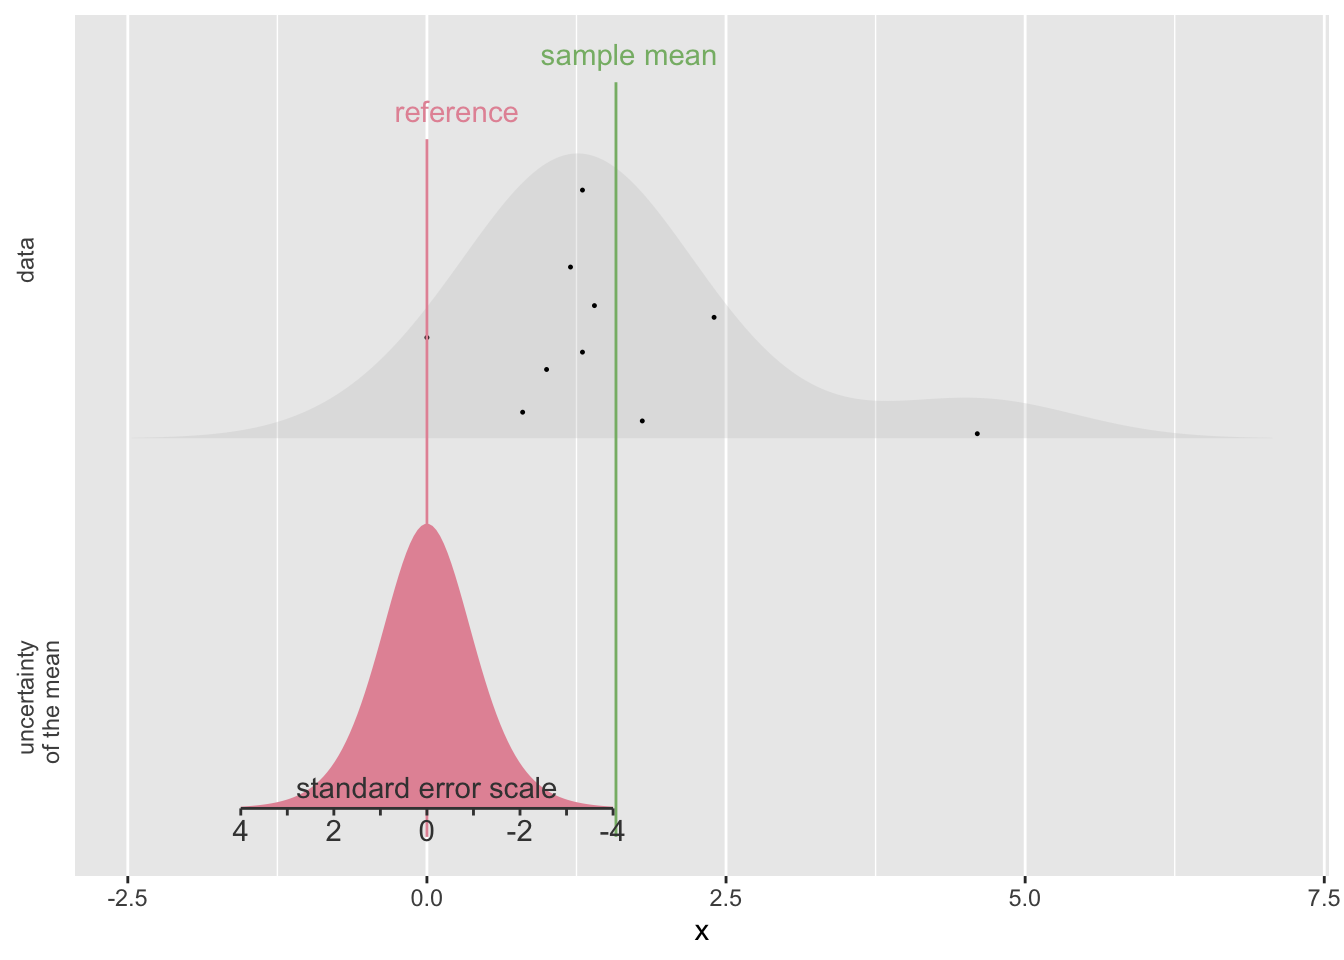
\includegraphics[width=0.49\linewidth]{book_files/figure-latex/sleep_ht-1} \end{center}

We view things through the eyes of the null hypothesis. If this is true then, most of the time, \(\bar x\) and \(\mu_0\) will be within 2 standard errors of one another. If we define the \emph{test statistic} to be
\[
      t = \frac{\bar{x} - \mu_0}{\mbox{s.e.}(\bar{x})}
\]
then we should expect \(-2 \leq t \leq 2\) most of the time. More precisely, \((\bar{x} - \mu_0) / \mbox{s.e.}(\bar{x})\) will follow a \(t\)-distribution with \((n-1)\) degrees of freedom.

Formal operation of a hypothesis test involves specifying the values of \(t\) which will lead us to reject the null hypothesis that \(\mu = \mu_0\). The left hand plot below shows a \(t\)-distribution with the tail areas corresponding to 2.5\% probability highlighted. This leaves 95\% of the distribution on the central area. If the test statistic \(t\) falls in the highlighted region then this is taken as evidence that the null hypothesis is implausible. In other words, there is significant evidence that the true mean is different from \(\mu_o\).

The plots can be reproduced by using the \texttt{rp.tables} function from the \texttt{rpanel} package.

\begin{Shaded}
\begin{Highlighting}[]
   \FunctionTok{rp.tables}\NormalTok{(}\AttributeTok{panel =} \ConstantTok{FALSE}\NormalTok{, }\AttributeTok{distribution =} \StringTok{"t"}\NormalTok{, }\AttributeTok{degf1 =} \DecValTok{24}\NormalTok{, }\AttributeTok{observed.value =} \StringTok{"2.5"}\NormalTok{,}
             \AttributeTok{tail.probability =} \StringTok{"fixed probability"}\NormalTok{)}
   \FunctionTok{rp.tables}\NormalTok{(}\AttributeTok{panel =} \ConstantTok{FALSE}\NormalTok{, }\AttributeTok{distribution =} \StringTok{"t"}\NormalTok{, }\AttributeTok{degf1 =} \DecValTok{24}\NormalTok{, }\AttributeTok{observed.value =} \StringTok{"2.5"}\NormalTok{,}
             \AttributeTok{tail.probability =} \StringTok{"from observed value"}\NormalTok{)}
\end{Highlighting}
\end{Shaded}

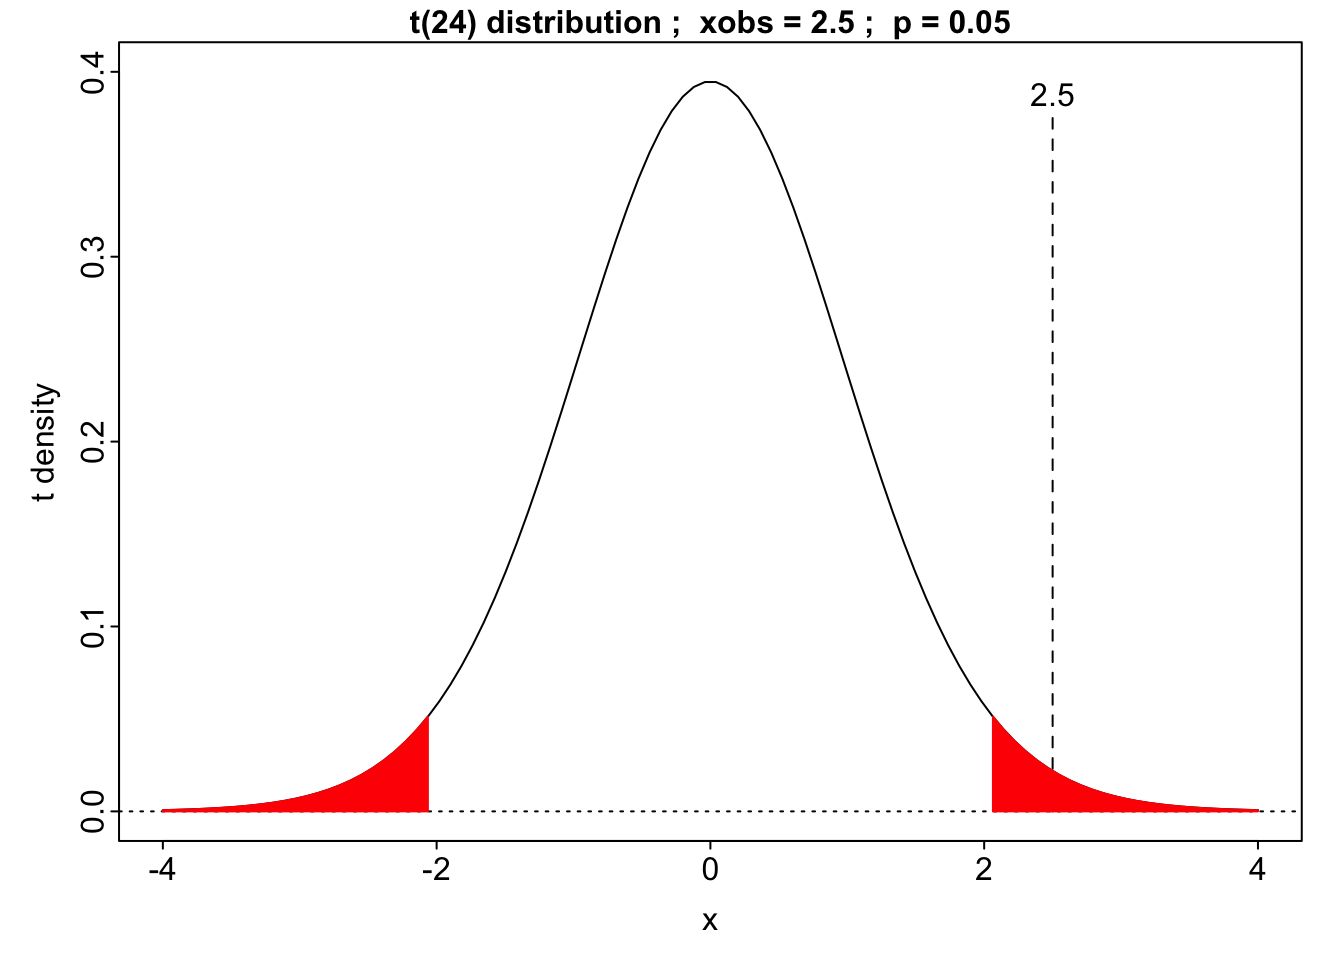
\includegraphics[width=0.5\linewidth]{book_files/figure-latex/hypothesis-tests-1} 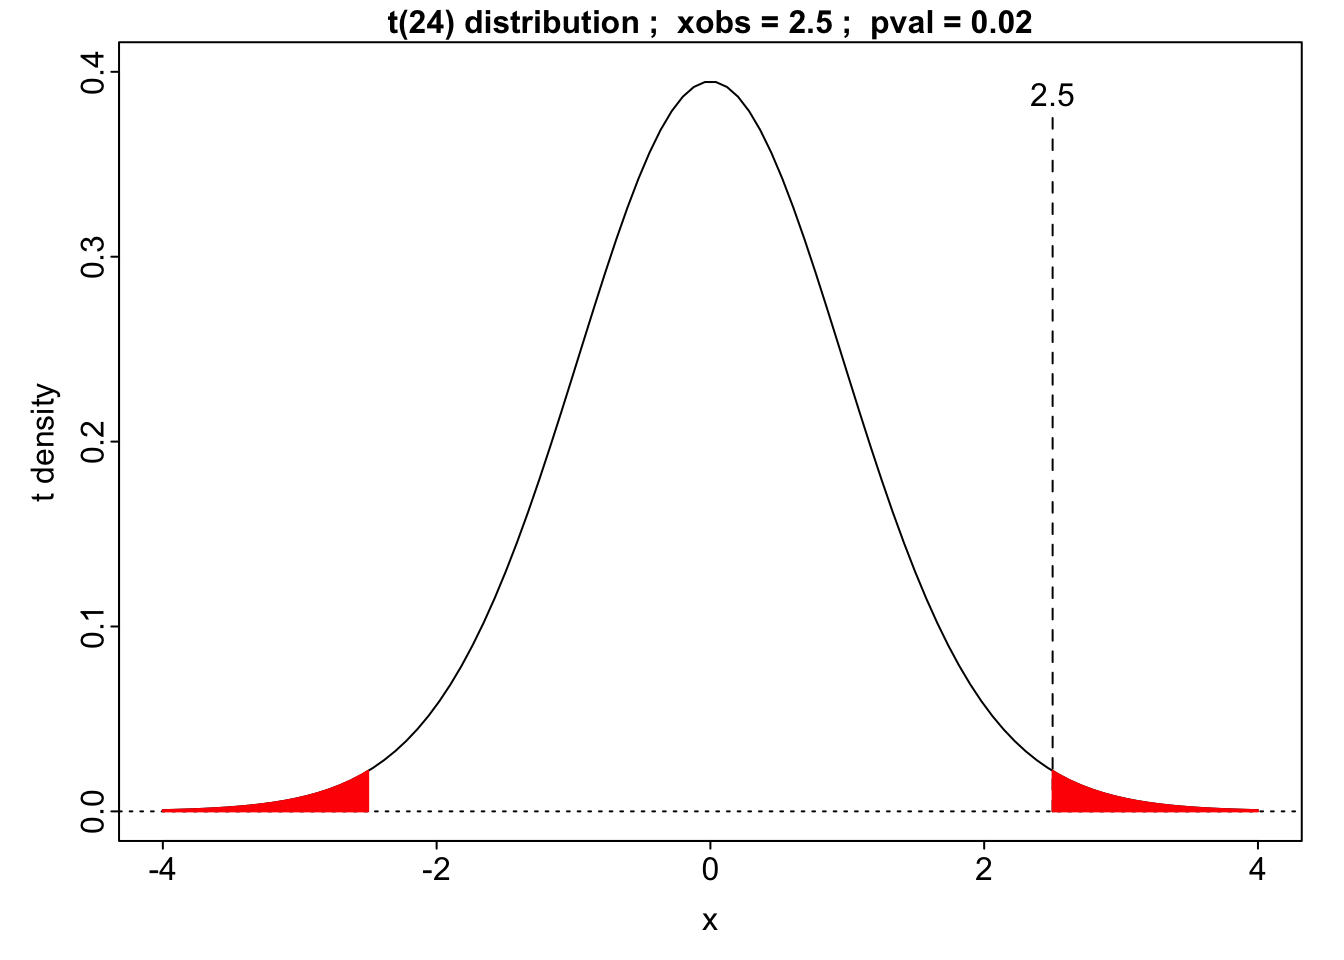
\includegraphics[width=0.5\linewidth]{book_files/figure-latex/hypothesis-tests-2}

There is an alternative way of quantifying the outcome of the test. We compare the observed value of the test statistic to the reference distribution by computing how much of the distribution is more extreme than the observed value. This is called the \emph{p-value}. If we did not specify in advance that the alternative involved only values below \(\mu_0\) or only values above \(\mu_0\) then we should measure extremity in both tails of the reference distribution. This is illustrated in the right hand plot above, where we see the p-value is 0.02. As this is less than the conventional threshold of 0.05, we again have significant evidence that the true value of the mean is not \(\mu_0\).

\section{Comparing two means}\label{comparing-two-means}

\section{Further reading}\label{further-reading-1}

M., D., and M. (\citeproc{ref-diez_2019_book}{2019})

Hubbard, Haig, and Parsa (\citeproc{ref-hubbard_2019_amerstat}{2019})

\section{Exercises}\label{quantifying-uncertainty-exercises}

\subsection{Standard errors}\label{standard-errors}

Use the \texttt{rp.sample} function to explore the phenomenon that \emph{most of the time, the true parameter and the estimate are within 2 standard errors}. Try setting the true mean and standard deviation to different values to confirm that this priniciple holds.

\chapter{Other approaches to inference}\label{other-approaches-to-inference}

\section{Computational inference}\label{computational-inference}

The problems we have discussed so far have been very simple once where theory can be worked out analytically to provide simple formulate and procedures. With more complex data structures, that can become much more difficult so this section will discuss some ways of approaching inference by computational means. The underlying principles are essentially the same but the method of implementation is different.

\subsection{Simulation methods}\label{simulation-methods}

There are some circumstances where the model whose suitability we wish to assess is completely known, without any dependence on unknown parameters. A simple example arises from spatial point patterns where we may wish to assess the evidence that the point pattern is generated by a process which is not simply uniform. The plot below shows data on large (breast height diameter \textgreater= 50cm) longleaf pine trees in a 200m x 200m sqaure of forest.

\begin{Shaded}
\begin{Highlighting}[]
\FunctionTok{library}\NormalTok{(spatstat)}
\NormalTok{x }\OtherTok{\textless{}{-}}\NormalTok{ longleaf}\SpecialCharTok{$}\NormalTok{x[longleaf}\SpecialCharTok{$}\NormalTok{marks }\SpecialCharTok{\textgreater{}=}\DecValTok{50}\NormalTok{]}
\NormalTok{y }\OtherTok{\textless{}{-}}\NormalTok{ longleaf}\SpecialCharTok{$}\NormalTok{y[longleaf}\SpecialCharTok{$}\NormalTok{marks }\SpecialCharTok{\textgreater{}=}\DecValTok{50}\NormalTok{]}
\FunctionTok{library}\NormalTok{(ggplot2)}
\FunctionTok{ggplot}\NormalTok{(}\AttributeTok{mapping =} \FunctionTok{aes}\NormalTok{(x, y)) }\SpecialCharTok{+} \FunctionTok{geom\_point}\NormalTok{()}
\end{Highlighting}
\end{Shaded}

\begin{center}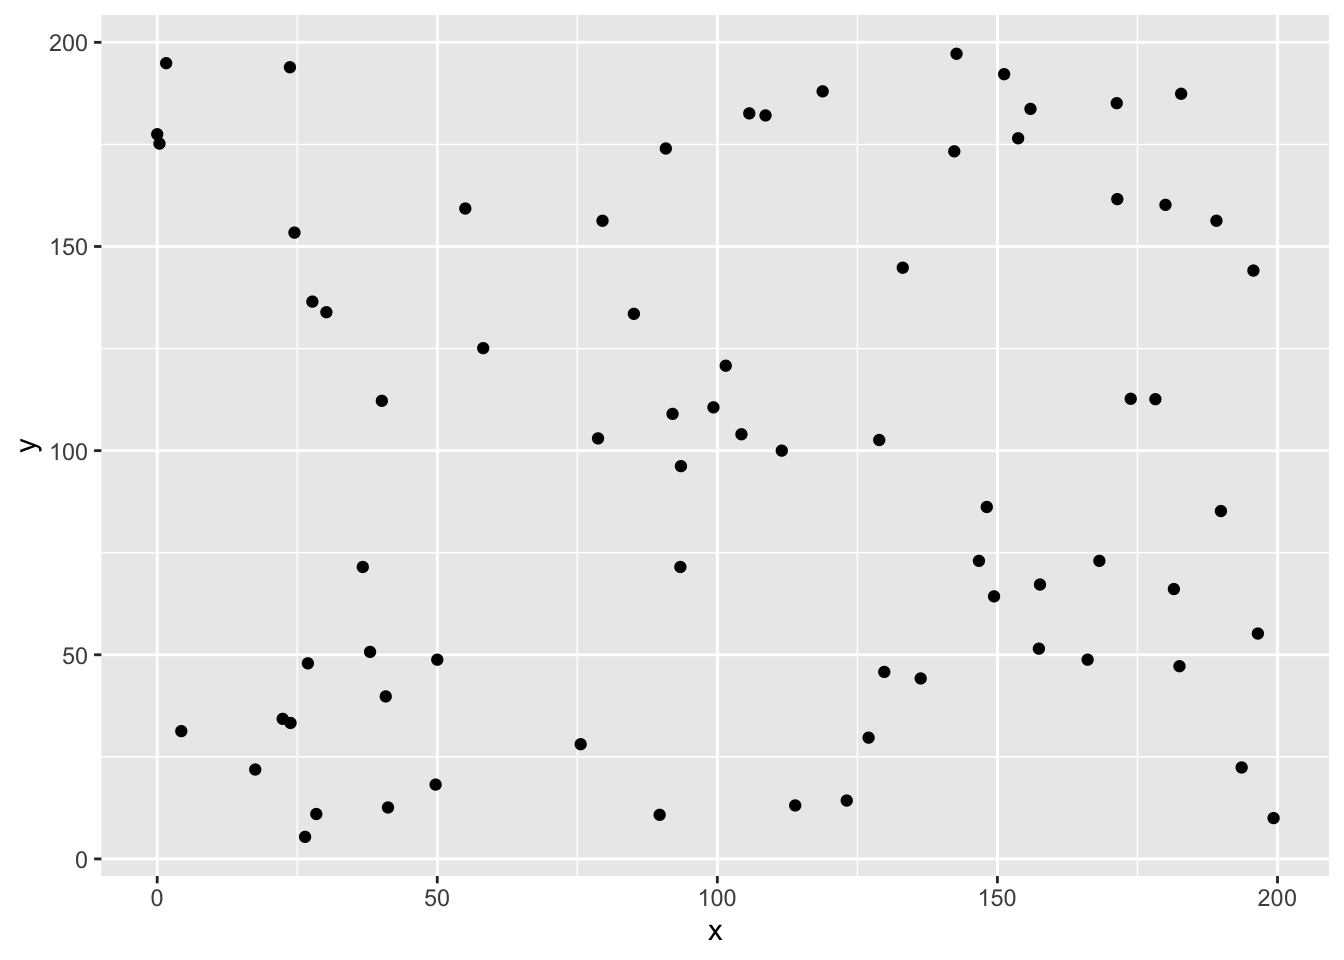
\includegraphics[width=0.7\linewidth]{book_files/figure-latex/unnamed-chunk-85-1} \end{center}

We can generate our own trees patterns in a uniform random manner simply by locating each tree at an x and y position each of which is generated uniformly in the range (0, 200). here are some examples of patterns generated in this way.

\begin{Shaded}
\begin{Highlighting}[]
\NormalTok{n }\OtherTok{\textless{}{-}} \FunctionTok{length}\NormalTok{(x)}
\ControlFlowTok{for}\NormalTok{ (i }\ControlFlowTok{in} \DecValTok{1}\SpecialCharTok{:}\DecValTok{3}\NormalTok{) \{}
\NormalTok{   plt }\OtherTok{\textless{}{-}} \FunctionTok{ggplot}\NormalTok{(}\AttributeTok{mapping =} \FunctionTok{aes}\NormalTok{(}\FunctionTok{runif}\NormalTok{(n, }\DecValTok{0}\NormalTok{, }\DecValTok{200}\NormalTok{), }\FunctionTok{runif}\NormalTok{(n, }\DecValTok{0}\NormalTok{, }\DecValTok{200}\NormalTok{))) }\SpecialCharTok{+}
            \FunctionTok{geom\_point}\NormalTok{()}
  \FunctionTok{print}\NormalTok{(plt)}
\NormalTok{\}}
\end{Highlighting}
\end{Shaded}

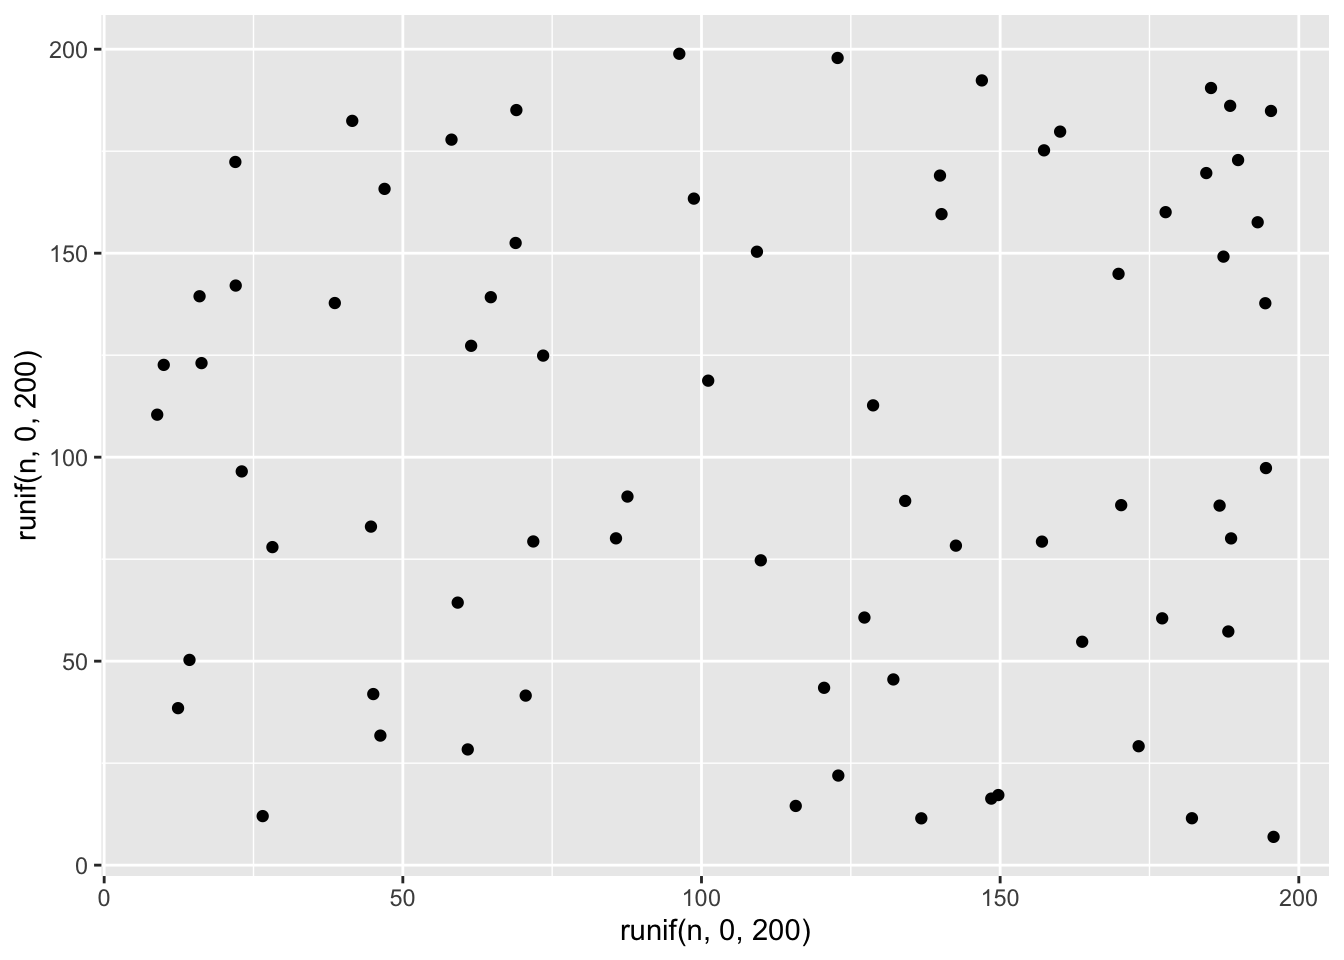
\includegraphics[width=0.32\linewidth]{book_files/figure-latex/unnamed-chunk-86-1} 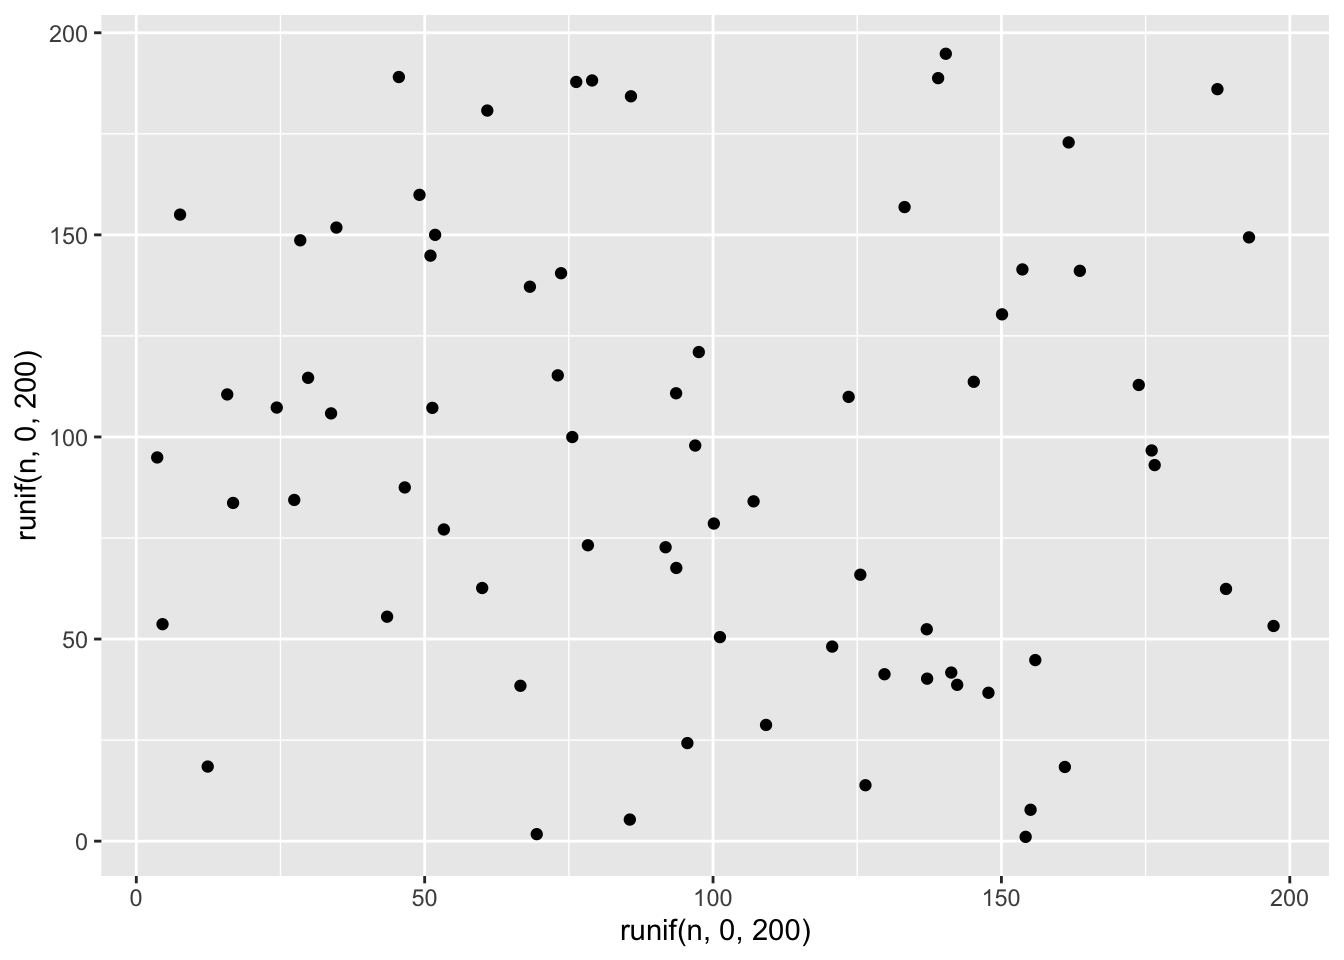
\includegraphics[width=0.32\linewidth]{book_files/figure-latex/unnamed-chunk-86-2} 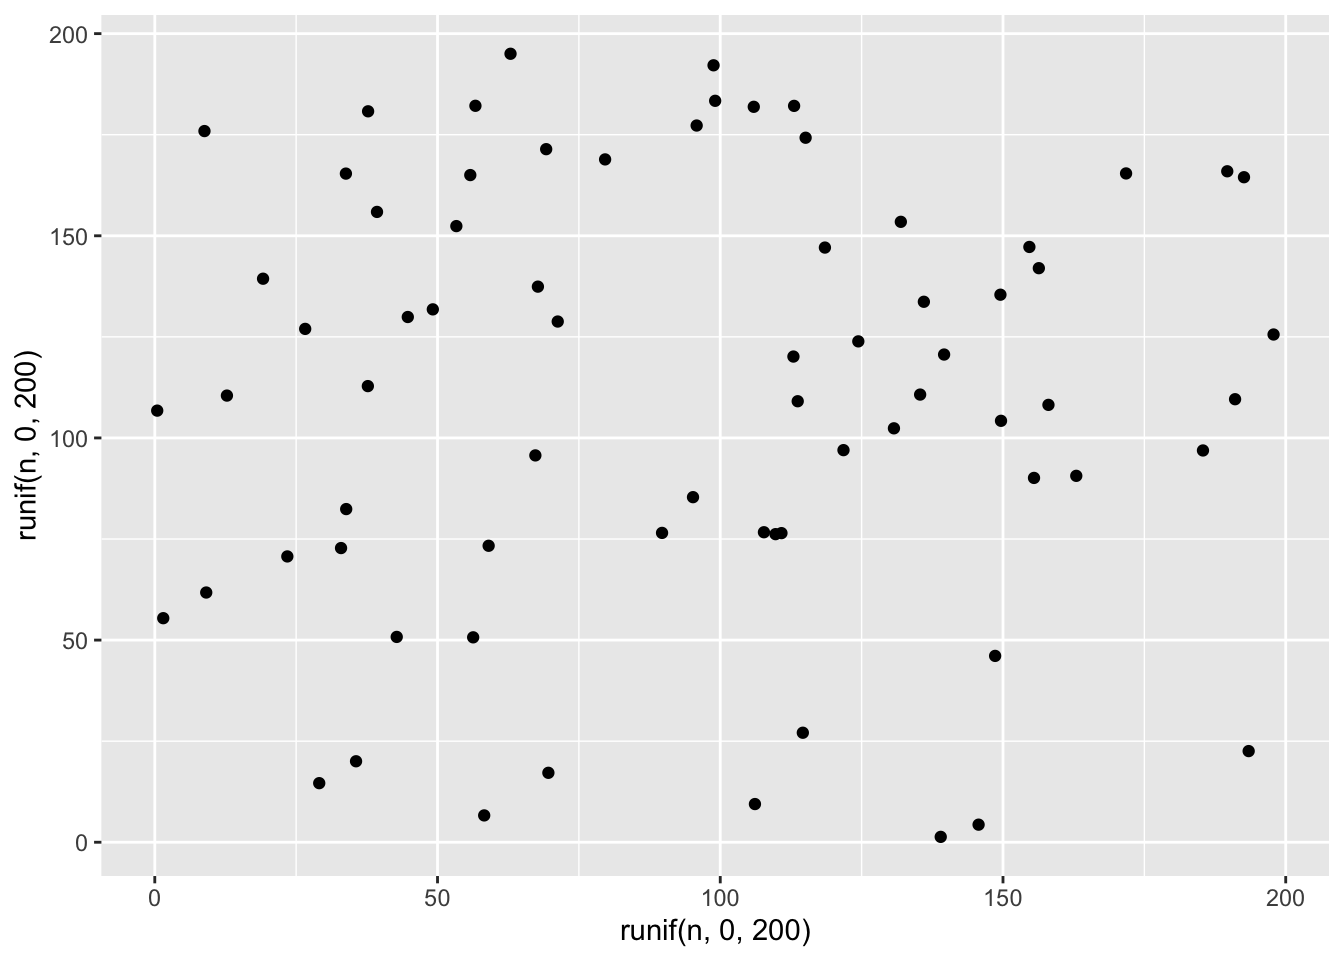
\includegraphics[width=0.32\linewidth]{book_files/figure-latex/unnamed-chunk-86-3}

How should we compare the observed pattern with the randomly generated ones? A simple way of doing this is to measure for each tree the distance to its nearest neighbour. If the pattern exhibits clustering, then these distances should be small, while if the pattern is uniform they will tend to be larger. We might then use as our test statistic the average of the distances to each nearest neighbour. We can generate the distribution of this average distance in the case where the locations are uniformly distributed simply by repeatedly simulating locations and retaining the average nearest neighbour distance for each one. The \texttt{nndist} function from the \texttt{spatstat} package can help us with the nearest neighbour distances.

\begin{Shaded}
\begin{Highlighting}[]
\NormalTok{nsim  }\OtherTok{\textless{}{-}} \DecValTok{10000}
\NormalTok{tstat }\OtherTok{\textless{}{-}} \FunctionTok{rep}\NormalTok{(}\DecValTok{0}\NormalTok{, nsim)}
\ControlFlowTok{for}\NormalTok{ (i }\ControlFlowTok{in} \DecValTok{1}\SpecialCharTok{:}\NormalTok{nsim) \{}
\NormalTok{  pp }\OtherTok{\textless{}{-}} \FunctionTok{cbind}\NormalTok{(}\FunctionTok{runif}\NormalTok{(n, }\DecValTok{0}\NormalTok{, }\DecValTok{200}\NormalTok{), }\FunctionTok{runif}\NormalTok{(n, }\DecValTok{0}\NormalTok{, }\DecValTok{200}\NormalTok{))}
\NormalTok{  tstat[i] }\OtherTok{\textless{}{-}} \FunctionTok{mean}\NormalTok{(}\FunctionTok{nndist}\NormalTok{(pp[ , }\DecValTok{1}\NormalTok{], pp[ , }\DecValTok{2}\NormalTok{]))}
\NormalTok{\}}
\NormalTok{tstat.obs }\OtherTok{\textless{}{-}} \FunctionTok{mean}\NormalTok{(}\FunctionTok{nndist}\NormalTok{(x, y))}
\FunctionTok{ggplot}\NormalTok{(}\AttributeTok{mapping =} \FunctionTok{aes}\NormalTok{(tstat)) }\SpecialCharTok{+} \FunctionTok{geom\_histogram}\NormalTok{() }\SpecialCharTok{+}
   \FunctionTok{geom\_vline}\NormalTok{(}\AttributeTok{xintercept =}\NormalTok{ tstat.obs, }\AttributeTok{col =} \StringTok{"red"}\NormalTok{)}
\FunctionTok{length}\NormalTok{(tstat[tstat }\SpecialCharTok{\textless{}}\NormalTok{ tstat.obs]) }\SpecialCharTok{/}\NormalTok{ nsim}
\end{Highlighting}
\end{Shaded}

\begin{verbatim}
## [1] 0.3141
\end{verbatim}

\begin{center}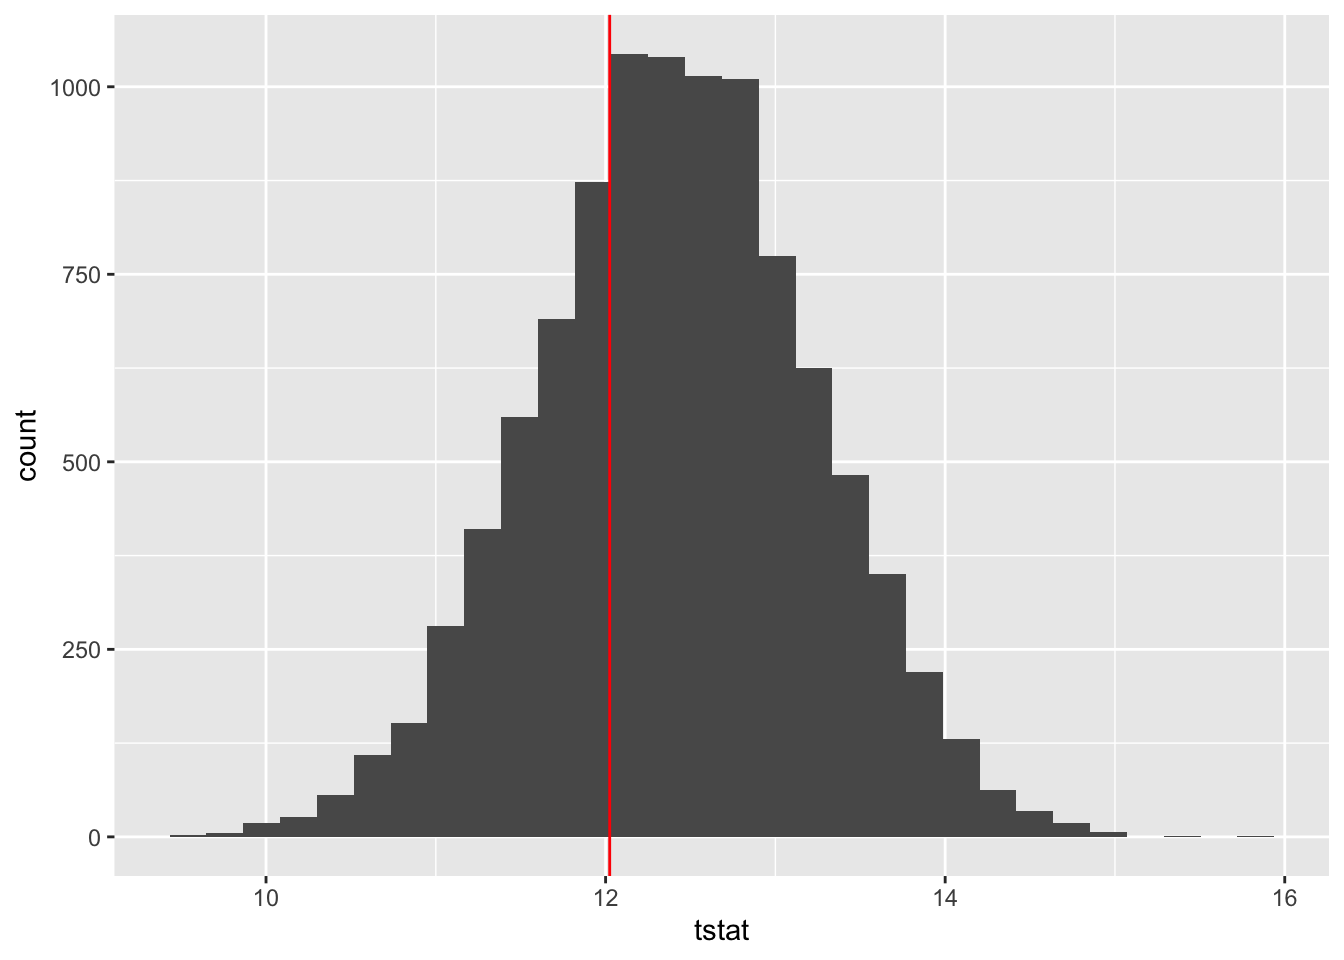
\includegraphics[width=0.7\linewidth]{book_files/figure-latex/unnamed-chunk-87-1} \end{center}

The histogram shows the distribution (subject to the variation present through simulation) of the average nearest neighbour distance when of atoms really are uniform. The red line shows the average neighbour distance for the observed data. Informally, but clearly, we can see that from this perspective the observed data is entirely consistent with the assumption of uniformity. An empirical p-value can be computed simply from the proportion of simulated values which fall below the observed one (as we look for evidence against uniformity in small nearest neighbour distances).

\subsection{Randomisation tests}\label{randomisation-tests}

Randomisation is very important principle in designing experiments as it helps to overcome issues of bias. We will consider this in detail elsewhere. Randomisation can also be used as the basis for analysis when we are reluctant to make the normality and independence assumptions which underlie standard methods. The dataset below provides a very simple example of this it refers to an experiment to assess the possibly different effects of two fertilisers applied to tomato plants growing in a row. (This example comes from the book \emph{Statistics for Experimenters} by Box, Hunter and Hunter.)

\begin{verbatim}
      Row position     1     2     3     4     5     6     7     8     9    10    11
      Fertiliser       A     A     B     B     A     B     B     B     A     A     B
      Yield (pounds) 29.9  11.4  26.6  23.7  25.3  28.5  14.2  17.9  16.5  21.1  24.3
\end{verbatim}

If the positions the fertilisers in the row have been randomised, and if the two fertilisers A and B are in fact equivalent in the effects, then the labels attached to the observations are immaterial. There is no connection between the labels and the outcomes. This allows us to calculate the distribution of the difference between the mean yields of A and B which is generated by the randomisation procedure. The histogram below shows this. For convenience (indeed, laziness!) it has been constructed from random permutations rather than the systematic list of all possible randomisations.

\begin{Shaded}
\begin{Highlighting}[]
\NormalTok{fertiliser }\OtherTok{\textless{}{-}} \FunctionTok{c}\NormalTok{(}\StringTok{"A"}\NormalTok{, }\StringTok{"A"}\NormalTok{, }\StringTok{"B"}\NormalTok{, }\StringTok{"B"}\NormalTok{, }\StringTok{"A"}\NormalTok{, }\StringTok{"B"}\NormalTok{, }\StringTok{"B"}\NormalTok{, }\StringTok{"B"}\NormalTok{, }\StringTok{"A"}\NormalTok{, }\StringTok{"A"}\NormalTok{, }\StringTok{"B"}\NormalTok{)}
\NormalTok{yield      }\OtherTok{\textless{}{-}} \FunctionTok{c}\NormalTok{(}\FloatTok{29.9}\NormalTok{, }\FloatTok{11.4}\NormalTok{, }\FloatTok{26.6}\NormalTok{, }\FloatTok{23.7}\NormalTok{, }\FloatTok{25.3}\NormalTok{, }\FloatTok{28.5}\NormalTok{, }\FloatTok{14.2}\NormalTok{, }\FloatTok{17.9}\NormalTok{, }\FloatTok{16.5}\NormalTok{, }\FloatTok{21.1}\NormalTok{, }\FloatTok{24.3}\NormalTok{)}
\NormalTok{nperm      }\OtherTok{\textless{}{-}} \DecValTok{1000}
\NormalTok{tstat      }\OtherTok{\textless{}{-}} \FunctionTok{rep}\NormalTok{(}\DecValTok{0}\NormalTok{, nperm)}
\ControlFlowTok{for}\NormalTok{ (i }\ControlFlowTok{in} \DecValTok{1}\SpecialCharTok{:}\NormalTok{nperm) \{}
\NormalTok{  smp      }\OtherTok{\textless{}{-}} \FunctionTok{sample}\NormalTok{(fertiliser)}
\NormalTok{  tstat[i] }\OtherTok{\textless{}{-}} \FunctionTok{diff}\NormalTok{(}\FunctionTok{tapply}\NormalTok{(yield, smp, mean))}
\NormalTok{\}}
\NormalTok{tstat.obs }\OtherTok{\textless{}{-}} \FunctionTok{diff}\NormalTok{(}\FunctionTok{tapply}\NormalTok{(yield, fertiliser, mean))}
\FunctionTok{ggplot}\NormalTok{(}\AttributeTok{mapping =} \FunctionTok{aes}\NormalTok{(tstat)) }\SpecialCharTok{+} \FunctionTok{geom\_histogram}\NormalTok{() }\SpecialCharTok{+}
   \FunctionTok{geom\_vline}\NormalTok{(}\AttributeTok{xintercept =}\NormalTok{ tstat.obs, }\AttributeTok{col =} \StringTok{"red"}\NormalTok{)}
\end{Highlighting}
\end{Shaded}

\begin{center}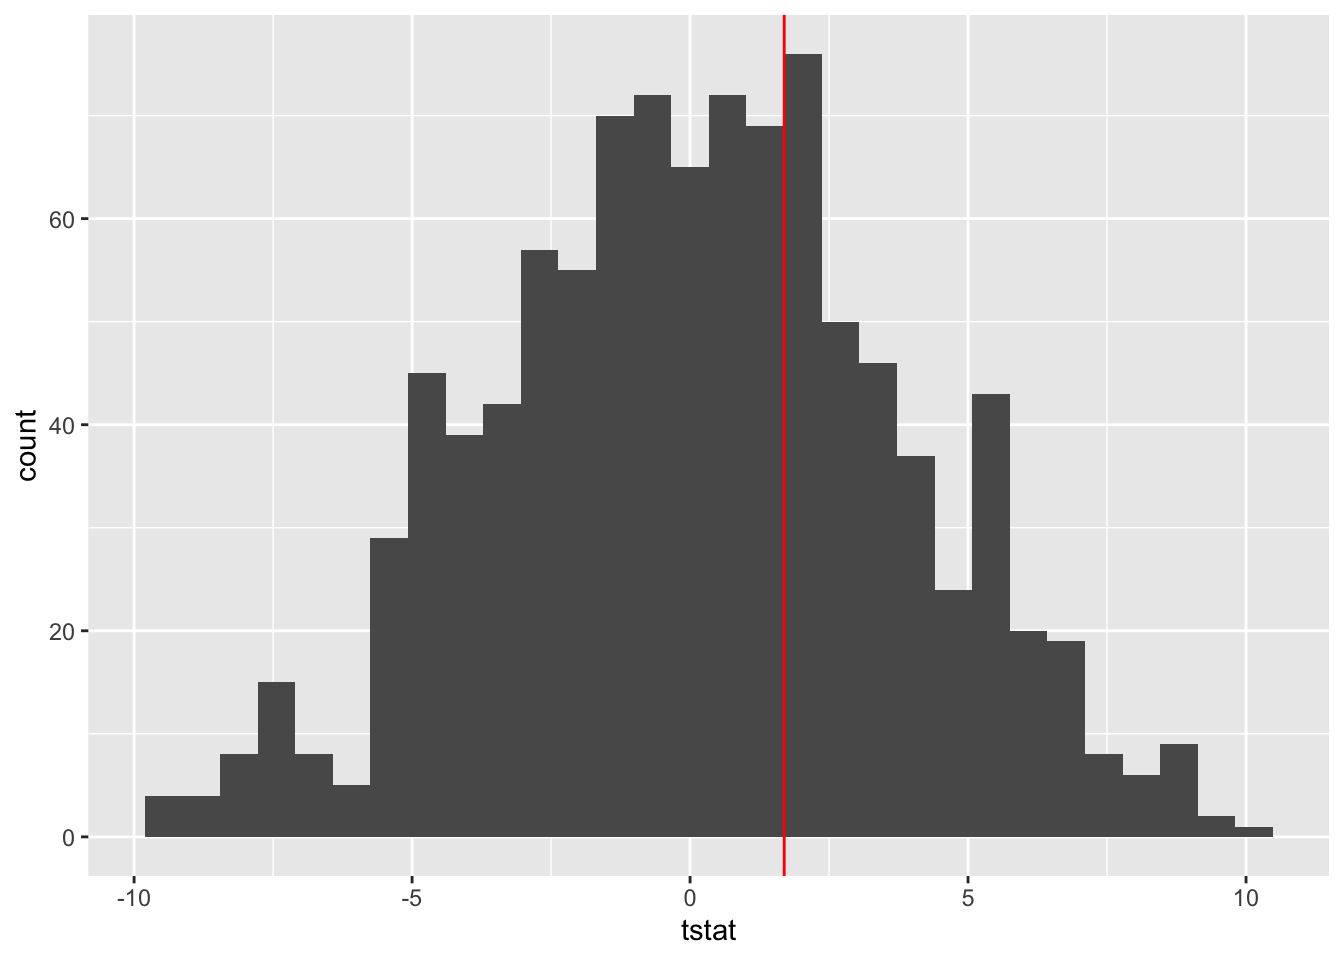
\includegraphics[width=0.7\linewidth]{book_files/figure-latex/unnamed-chunk-88-1} \end{center}

There are several new functions used in the \texttt{R} code here (\texttt{c}, \texttt{diff}, \texttt{tapply}). You will hopefully feel ready to explore these through the help system by this stage. The end result is a histogram which represents the distribution, induced by randomisation, of the mean sample difference between A and B when the two treatments have identical effects. When we compare this with the observed mean difference it is clear that the two are compatible. So there is no evidence that A and B have different effects. If required, a p-value could be obtained by the means discussed in the simulation test section above. However, the conclusion is already clear.

\subsection{The bootstrap}\label{the-bootstrap}

We generally regard observed data as having been generated by some underlying distribution. If we construct an estimator of some quantity of interest, such as a population mean, then we need to know how accurate estimate is as a guide to the true value. The simple but surprising idea behind the bootstrap is that we mimic the variation of the sample around the distribution by the variation of resampled datasets around our original sample. When the bootstrap was first proposed in the 1970s, it took people by surprise but in fact it can be shown to be well founded theoretically.

Suppose we are dealing with a distribution which has long tails. In other words, we may find that outliers (unusually large or small observations) are often present in sample datasets. Methods based on the assumption of a normal distribution will be strongly affected by this. A simple device is to compute a \emph{trimmed mean}. This simply computes the main of the remaining data after a proportion of the highest and lowest observations has been removed. This is an attractive way of defending against the effect of long tails, but how do we quantify the uncertainty of our sample estimator as a guide to the true trimmed mean of the underlying distribution?

The bootstrap takes the observed sample and resamples the data with replacement. A trimmed mean is calculated on each resample. In the simplest approach to construction of a confidence interval, this is generated simply through percentiles of the trimmed means generated by resampling. The example below shows the mechanics of this, using a simple normal random sample to represent the observed data.

\begin{Shaded}
\begin{Highlighting}[]
\NormalTok{x      }\OtherTok{\textless{}{-}} \FunctionTok{rnorm}\NormalTok{(}\DecValTok{25}\NormalTok{)}
\NormalTok{tm.obs }\OtherTok{\textless{}{-}} \FunctionTok{mean}\NormalTok{(x, }\AttributeTok{trim =} \FloatTok{0.1}\NormalTok{)}

\NormalTok{nboot  }\OtherTok{\textless{}{-}} \DecValTok{10000}
\NormalTok{tmdiff }\OtherTok{\textless{}{-}} \FunctionTok{rep}\NormalTok{(}\DecValTok{0}\NormalTok{, nboot)}
\ControlFlowTok{for}\NormalTok{ (i }\ControlFlowTok{in} \DecValTok{1}\SpecialCharTok{:}\NormalTok{nboot)}
\NormalTok{   tmdiff[i] }\OtherTok{\textless{}{-}} \FunctionTok{mean}\NormalTok{(}\FunctionTok{sample}\NormalTok{(x, }\AttributeTok{replace =} \ConstantTok{TRUE}\NormalTok{), }\AttributeTok{trim =} \FloatTok{0.1}\NormalTok{) }\SpecialCharTok{{-}}\NormalTok{ tm.obs}
\NormalTok{tm.obs }\SpecialCharTok{{-}} \FunctionTok{quantile}\NormalTok{(tmdiff, }\FunctionTok{c}\NormalTok{(}\FloatTok{0.975}\NormalTok{, }\FloatTok{0.025}\NormalTok{))}
\end{Highlighting}
\end{Shaded}

\begin{verbatim}
##      97.5%       2.5% 
## -0.6245322  0.1898431
\end{verbatim}

\section{Bayesian inference}\label{bayesian-inference}

The methods which have been described in this course have a very long and well established history. They are in widespread use and have brought insight to an enormous array of applications across the board. From a philosophical point of view these methods are referred to as \emph{frequentist}. The name comes from the idea of continued sampling of data, under the same conditions, for which it can be shown that relative frequencies converge eventually to probabilities.

An alternative approach to inference is to consider the uncertainty associated with quantities of interest such as parameters, expressed not only through a model for the observed data but also through a prior distribution for the unknown parameters. Sometimes that prior information can be informative, based on knowledge or data about the situation being modelled. Sometimes the prior information can be vague or uninformative. Bayesian thinking allows uncertainty to be expressed as a combination of these two things, in a posterior distribution. A major step forward took place in the 1990s when computational methods of deriving posterior distributions were developed. For the first time this allowed complex problems to be handled by Bayesian models, with the attractive property that uncertainty at different levels can be propagated to generate posterior uncertainty about the quantities of interest, incorporating all the appropriate sources of uncertainty. This has led to extremely powerful tools for complex systems.

Treatment of this topic is beyond the scope of the current course.

\section{Exercises}\label{exercises-1}

\subsection{Coverage property of bootstrap confidence intervals}\label{coverage-property-of-bootstrap-confidence-intervals}

During the session an example of a confidence interval for a trimmed mean was discussed. Write some code to evaluate the \emph{coverage} of this method of constructing a confidence interval. You can do this by repeatedly simulating sample from the true distribution (\texttt{rnorm(25)}), constructing a bootstrap confidence interval using the code discussed, and counting how many times the calculated confidence interval covers the true value (0).

\chapter{Inference with categorical data}\label{inference-with-categorical-data}

So far, we have considered data measured on a continuous scale but there are, of course, many other types of data structure. Here we will deal with data in the form of categories.

\section{Simple proportions}\label{simple-proportions}

We often encounter problems where:

\begin{itemize}
\tightlist
\item
  the number of items in the sample, denoted by \(n\), is fixed in advance;
\item
  there are two possible outcomes for each item (yes/no, success/failure, etc.);
\item
  each item has the same chance of producing a `success', independently of all other items.
\end{itemize}

This leads to the \emph{Binomial} model which describes the probabilities of the number of `successes' out of the \(n\) items, when the probability of success for a single item is \(p\).

If the number of `successes' in the sample of size \(n\) is \(x\) then a natural estimate of
\(p\) is the \emph{sample proportion}, \(x/n\). We write:
\[
                  \hat{p} = x/n
\]

We need to quantify the uncertainty associated with estimating \(p\) by \(\hat{p}\). As usual, the \emph{standard error} does this for us.

The plot below uses simulation to show the variation in \(\hat{p}\) when samples of size \(n\) are repeatedly drawn from populations where the true proportion if \(p\). You might like to experiment with this code tp see the effectsd of changing \texttt{n} and \texttt{p}.

\begin{Shaded}
\begin{Highlighting}[]
\NormalTok{n }\OtherTok{\textless{}{-}} \DecValTok{10}
\NormalTok{p }\OtherTok{\textless{}{-}} \FloatTok{0.5}
\NormalTok{x }\OtherTok{\textless{}{-}} \FunctionTok{rbinom}\NormalTok{(}\DecValTok{1000}\NormalTok{, n, p) }
\FunctionTok{hist}\NormalTok{(x }\SpecialCharTok{/}\NormalTok{ n, }\AttributeTok{col =} \StringTok{\textquotesingle{}grey\textquotesingle{}}\NormalTok{, }\AttributeTok{xlim =} \FunctionTok{c}\NormalTok{(}\DecValTok{0}\NormalTok{, }\DecValTok{1}\NormalTok{), }\AttributeTok{main =} \FunctionTok{paste}\NormalTok{(}\StringTok{\textquotesingle{}n =\textquotesingle{}}\NormalTok{, n, }\StringTok{\textquotesingle{}  p =\textquotesingle{}}\NormalTok{, p))}
\FunctionTok{abline}\NormalTok{(}\AttributeTok{v =}\NormalTok{ p, }\AttributeTok{col =} \StringTok{\textquotesingle{}red\textquotesingle{}}\NormalTok{)}
\end{Highlighting}
\end{Shaded}

\begin{center}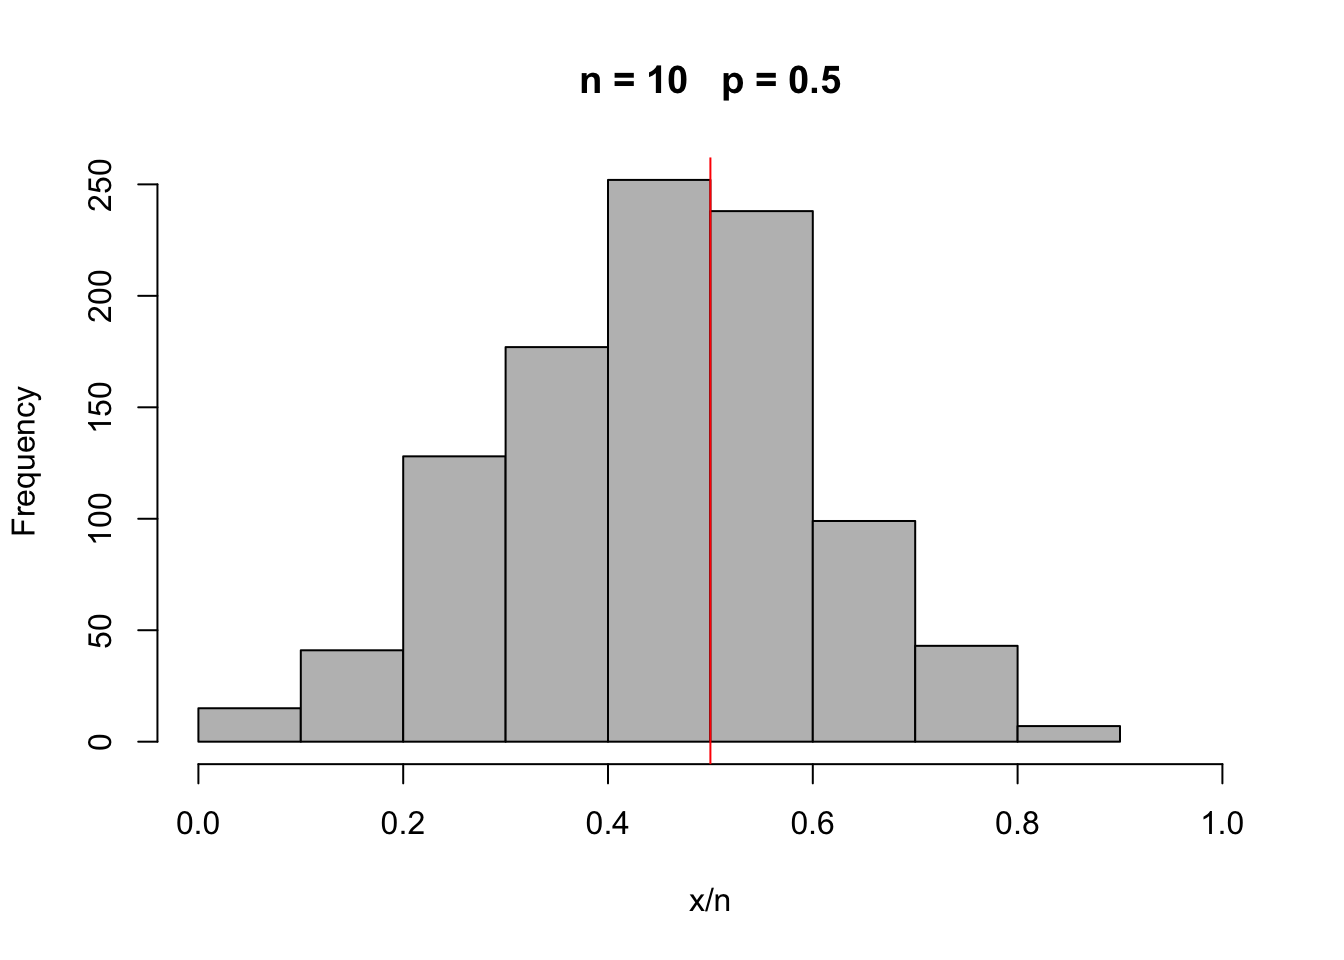
\includegraphics[width=0.5\linewidth]{book_files/figure-latex/unnamed-chunk-106-1} \end{center}

There are two simple points to note:

\begin{itemize}
\tightlist
\item
  The sample proportion is subject to error but it is centred
  on the true proportion in the population.
\item
  The size of the error in the sample proportion decreases as the
  size of the sample increases.
\end{itemize}

In fact it is possible to show that the variance of \(\hat{p}\) is \(p (1 - p) / n\). We can estimate the unknown \(p\) in this expression to obtain the standard error
\[
        s.e.(\hat{p}) = \sqrt{\hat{p}(1-\hat{p})/n}
\]
As in other cases, we should find that most of the sample proportions lie within two standard errors of the true proportion. In this case we do not have an exact result for a confidence interval, as we do with the Normal model, but an approximate 95\% confidence interval for \(p\) is easily obtained as
\[
                \hat{p} \pm 2 \mbox{s.e.}(\hat{p})
\]
In a \href{https://publications.parliament.uk/pa/ld201719/ldselect/ldppdm/106/10616.htm}{briefing note} for journalists, the UK Parliament provides a helpful guide to opinion polls. (The document was prepared by Peter Kellner for the British Polling Council.) This refers to an accuracy of 3\% in the main percentages reported in a poll based on 1000 respondents. Where does 3\% come from?

When the sample size is 1000, the standard error of a proportion is \(\sqrt{\hat{p}(1-\hat{p})/1000}\). The largest possible value of \(\hat{p}(1-\hat{p})\) is when \(\hat{p} = 0.5\), so the upper limit on the standard error is \(\sqrt{0.5 \times 0.5 / 1000} = 0.16\). Two standard errors is then 0.032, or around 3\%.

This is a useful guide, but there are many other aspects of this to consider. We are often interested in comparing the proportions from different categories, such as support for the main parties in an election, and the uncertainty will be increased when two proportions are involved. In addition, there are all the usual issues about the extent to which the sampling is genuinely random or subject to bias of various kinds. Nonetheless, the ability of standard error to help in quantifying uncertainty is helpful.

\section{Comparing proportions}\label{comparing-proportions}

\begin{quote}
\begin{center}\rule{0.5\linewidth}{0.5pt}\end{center}

\textbf{Example: Smoking and lung cancer}\\
In a famous historical study of the association between smoking and lung cancer, Doll \& Hill compared the numbers of smokers and non-smokers in samples of lung cancer patients and controls. The data for females are shown below.

\begin{verbatim}
                              cases  controls
                     smokers    41      28
                non-smokers     19      32
\end{verbatim}

Is there evidence of a link between smoking and lung cancer?

\begin{center}\rule{0.5\linewidth}{0.5pt}\end{center}
\end{quote}

Details of how these data were collected are given in the paper. There are interesting questions here about what constitutes an appropriate control group. In fact other hospital patients, not suffering from lung cancer, were used.

The principal question of interest is whether the proportion of smokers among the cases is different from the proportion of smokers among the controls.
We denote the underlying true proportion among the cases and controls by \(p_1\) and \(p_2\) respectively, with corresponding sample sizes \(n_1\) and \(n_2\). We can estimate the true proportions by the sample proportions,
\begin{eqnarray*}
        \hat{p}_1 = 41/60 = 0.683 \\
        \hat{p}_1 = 28/60 = 0.467
\end{eqnarray*}
We can also calculate the standard error of each sample proportion as
\begin{eqnarray*}
        \mbox{se}_1 & = & \sqrt{\hat{p}_1(1-\hat{p}_1)/n_1}
                      =  \sqrt{0.683 \times 0.317 / 60}
                      =  0.060 \\
        \mbox{se}_2 & = & \sqrt{\hat{p}_1(1-\hat{p}_1)/n_1}
                      =  \sqrt{0.467 \times 0.533 / 60}
                      =  0.064
\end{eqnarray*}

However, it is the \emph{difference} between the two groups which is of interest to us. We have a natural estimate in the differences of the proportions \(p_1-p_2\) in the difference of the sample proportions
\[
        \hat{p}_1 - \hat{p}_2  = 0.683 - 0.467 = 0.216 .
\]
We can also calculate the standard error of this difference by combing the individual standard errors, as follows:
\begin{eqnarray*}
        \mbox{se}_{\mbox{difference}} & = &
                \sqrt{\mbox{se}_1^2 + \mbox{se}_2^2}
\end{eqnarray*}
Notice that the squared standard errors are added together, despite the fact that the estimates of the proportions are being subtracted. This is because we are measuring the uncertainty involved and so the uncertainty of the difference combines the uncertainties of the individual components. With the present data this gives
\[
        \mbox{se}_{\mbox{difference}} = \sqrt{0.060^2 + 0.064^2}
                                = 0.088
\]
A \(95\%\) confidence interval for the difference in proportions is then:
\begin{eqnarray*}
        0.216 \pm 2 \times 0.088  \\
        \mbox{i.e.}  0.216 \pm 0.176 \\
        \mbox{i.e.}  (0.040, 0.392)
\end{eqnarray*}
Since this confidence interval does not contain \(0\), we therefore have
clear evidence that the proportions of smokers in the cases and control groups are different.

\section{Contingency tables}\label{contingency-tables}

The data on smoking and lung cancer can also be treated as a simple example of a \emph{contingency table}, which cross-classifies counts by two different factors. In fact, this was how the data were viewed in the original paper by Doll \& Hill. The method of analysis we will explore can be implemented in contingency tables with any number of rows or columns.

As ever, a helpful first step is to visualise the data, even when this consists of a very simple tabluation. The mosiacplot discussed earlier helps with this. The columns of the plot refer to the case and control groups. Here these are equal in size (60) but differences in in numbers would have been reflected in the width of the columns. This means that the height of each block now refers to proprtions of observations within each column.

\begin{Shaded}
\begin{Highlighting}[]
\NormalTok{x }\OtherTok{\textless{}{-}} \FunctionTok{matrix}\NormalTok{(}\FunctionTok{c}\NormalTok{(}\DecValTok{41}\NormalTok{, }\DecValTok{19}\NormalTok{, }\DecValTok{28}\NormalTok{, }\DecValTok{32}\NormalTok{), }\AttributeTok{ncol =} \DecValTok{2}\NormalTok{,}
            \AttributeTok{dimnames =} \FunctionTok{list}\NormalTok{(}\FunctionTok{c}\NormalTok{(}\StringTok{"smoker"}\NormalTok{, }\StringTok{"non{-}smoker"}\NormalTok{),}
                            \FunctionTok{c}\NormalTok{(}\StringTok{"cases"}\NormalTok{, }\StringTok{"controls"}\NormalTok{)))}
\FunctionTok{rp.contingency}\NormalTok{(x)}
\end{Highlighting}
\end{Shaded}

\begin{center}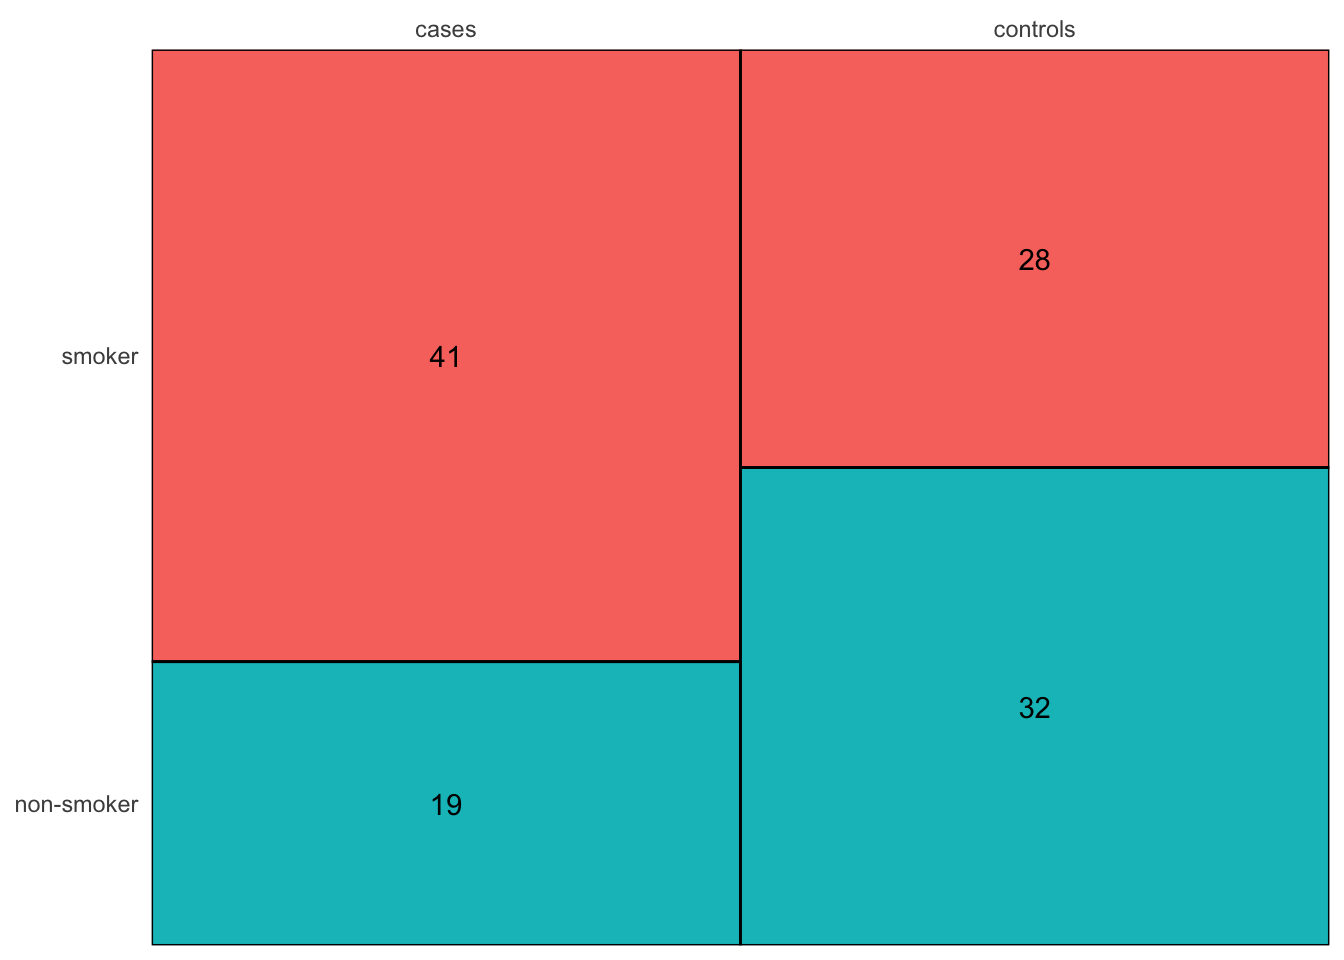
\includegraphics[width=0.7\linewidth]{book_files/figure-latex/smoking_mosaic-1} \end{center}

If there is no association between smoking and lung cancer, then the proportions associated with each column will be identical. We can use this idea to calculate \emph{expected values}, which describe the pattern we expect to see if the null hypothesis of no association is correct. Estimates of the common probabilities for each column are (69/120, 51/120) = (0.575, 0.425). The expected values by row are therefore obtained by multiplying the column totals by these probabilities. It so happens that the column totals are identical in this dataset, namely 60.

\begin{verbatim}
                            60 * 0.575, 60 * 0.575 = 34.5, 34.5
                            60 * 0.425, 60 * 0.425 = 25.5, 25.5
\end{verbatim}

We can now compare this table of expected values (\(E_{ij}\)) with the table of observed values (\(O_{ij}\)) above. We do this through a quantity known as the chi-squared statistic, defined as
\[
      \sum_{ij} \frac{(O_{ij} - E_{ij})^2}{E_{ij}}
\]

where the subscripts \(i\) and \(j\) index the rows and columns. The chi-squared statistic for the current dataset is \(5.76\).

This value is meaningful only when we compare it to a reference distribution. The theory for this setting tells us that the relevant comparison is with a \(\chi^2\) distribution, which is plotted below. This distribution is indexed by a parameter known as the \emph{degrees of freedom}. For contingency tables with \(r\) rows and \(c\) columns, the degrees of freedom should be set to \((r-1)(c-1)\), which in the current case is \(1\).

\begin{Shaded}
\begin{Highlighting}[]
\FunctionTok{library}\NormalTok{(rpanel)}
\FunctionTok{rp.tables}\NormalTok{(}\AttributeTok{panel =} \ConstantTok{FALSE}\NormalTok{, }\AttributeTok{distribution =} \StringTok{"chi{-}squared"}\NormalTok{, }\AttributeTok{degf1 =} \DecValTok{1}\NormalTok{, }\AttributeTok{observed.value =} \FloatTok{5.76}\NormalTok{)}
\end{Highlighting}
\end{Shaded}

\begin{center}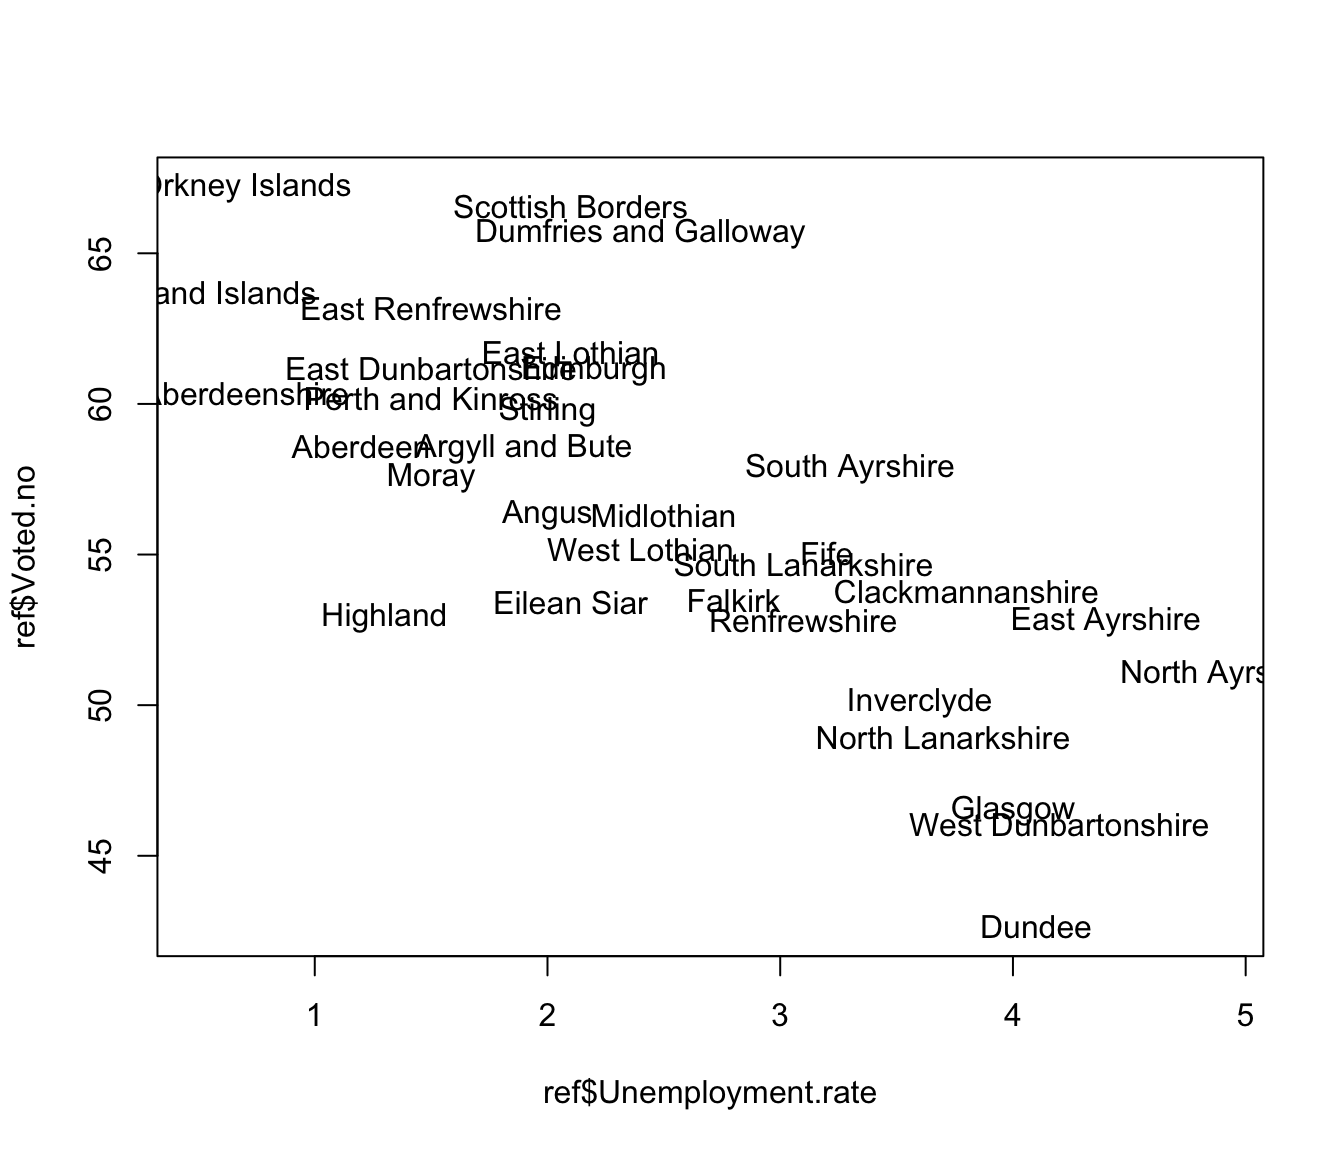
\includegraphics[width=0.6\linewidth]{book_files/figure-latex/unnamed-chunk-110-1} \end{center}

The observed value of the test statistic, which is also shown in the plot, is much higher than values we expect to see from this reference distribution. The upper 5\% point of the distribution is 3.84, which gives us a specific benchmark. We therefore have significant evidence that the proportions of smokers are different in the cases and controls. This formn of analysis has, unsurprisingly, confirmed the conclusions of the comparison of proportions in the previous section.

The chi-squared test can be easily implemented in \texttt{R} through the \texttt{chisq.test} function. By default this includes a correction for 2x2 tables in order to improve the accuracy of the reference distribution. However, the conclusion is unchanged.

\begin{Shaded}
\begin{Highlighting}[]
\FunctionTok{chisq.test}\NormalTok{(x)}
\end{Highlighting}
\end{Shaded}

\begin{verbatim}
## 
##  Pearson's Chi-squared test with Yates' continuity correction
## 
## data:  x
## X-squared = 4.9105, df = 1, p-value = 0.02669
\end{verbatim}

\section{Exercises}\label{exercises-2}

\subsection{Opinion polls}\label{opinion-polls}

Opionion polls reported in newspapers are sometimes treated with scepticism. This is particularly true of polls published before general elections! The \emph{Independent} newspaper ran a series of articles on this some time ago. In particular, it was claimed that,in \emph{`a sample of \(1000\) people, the main percentages should be accurate \ldots{} to within three percent, nineteen times out of twenty'}.

Is this correct? How can it be justified? Use the formula for the standard error of a proportion to think this through.

\subsection{Respiratory disease in infancy}\label{respiratory-disease-in-infancy}

Holland, Bailey \& Bland (1978, \emph{Journal of Epidemiology and Community Health}) reported on a study of the effects of bronchitis in infancy on the occurrence of respiratory problems later in life. The following table reports the occurrence of these events in a sample which was studied by the authors.

\begin{tabular}{r|r|r}
\hline
 & Cough at 14 & No cough at 14\\
\hline
Bronchitis at 5 & 26 & 247\\
\hline
No bronchitis at 5 & 44 & 1002\\
\hline
\end{tabular}

Is there evidence of a link?

\subsection{Smoking and lung cancer}\label{smoking-and-lung-cancer}

The earlier analysis used a chi-squared test to assess the evidence that the proportion of smokers is different in cases and controls. Construct a confidence interval for the difference of these proportions as an alternative approach, making sure that you understand how to interpret the interval you produce.

\subsection{Confidence intervals and p-values}\label{confidence-intervals-and-p-values}

In the two examples above, both confidence intervals and hypothesis tests have now been used. These should be equivalent in terms of the evidence for the presence of an effect. What are the relative merits of the confidence interval and hypothesis testing approaches in this context?

\phantomsection\label{refs}
\begin{CSLReferences}{1}{0}
\bibitem[\citeproctext]{ref-bhatt_2010_perspclinres}
Bhatt, Arun. 2010. {``Evolution of Clinical Research: A History Before and Beyond James Lind.''} \emph{Perspectives in Clinical Research} 1 (1): 6.

\bibitem[\citeproctext]{ref-bowman-1994-teachingstatistics}
Bowman, A. W. 1994. {``Teaching by Design.''} \emph{Teaching Statistics} 16: 2--4. \url{https://doi.org/10.1111/j.1467-9639.1994.tb00670.x}.

\bibitem[\citeproctext]{ref-diggle_2011_book}
Diggle, Peter J, and Amanda Chetwynd. 2011. \emph{Statistics and Scientific Method: An Introduction for Students and Researchers}. Oxford University Press.

\bibitem[\citeproctext]{ref-hubbard_2019_amerstat}
Hubbard, Raymond, Brian D Haig, and Rahul A Parsa. 2019. {``The Limited Role of Formal Statistical Inference in Scientific Inference.''} \emph{The American Statistician} 73 (sup1): 91--98.

\bibitem[\citeproctext]{ref-diez_2019_book}
M., Diez D., Barr C. D., and Çetinkaya-Rundel M. 2019. \emph{OpenIntro Statistics}. 4th edition. \href{https://openintro.org/os}{openintro.org/os}.

\bibitem[\citeproctext]{ref-mackay_2000_statsci}
MacKay, R Jock, and R Wayne Oldford. 2000. {``Scientific Method, Statistical Method and the Speed of Light.''} \emph{Statistical Science}, 254--78. \url{https://www.jstor.org/stable/2676665}.

\bibitem[\citeproctext]{ref-marshall_1948_bmj}
Marshall, Geoffrey, J. W. S. Blacklock, C. Cameron, N. B. Capon, R. Cruickshank andJ. H. Gaddum, F. R. G. Heaf, A. Bradford Hill, et al. 1948. {``Streptomycin Treatment of Pulmonary Tuberculosis.''} \emph{British Medical Journal}, 769--82.

\bibitem[\citeproctext]{ref-rosling_2018_book}
Rosling, Hans. 2018. \emph{Factfulness}. London: Hodder \& Stoughton.

\end{CSLReferences}

\end{document}
